%
%  sst_index_draft
%
%  Created by James on 2012-05-14.
%  Copyright (c) 2012 __MyCompanyName__. All rights reserved.
%
\documentclass[]{article}
%\documentclass[a4paper, 10pt]{article}

% Use utf-8 encoding for foreign characters
\usepackage[utf8]{inputenc}

% Setup for fullpage use
%\usepackage{fullpage}

% Uncomment some of the following if you use the features
%
% Running Headers and footers
%\usepackage{fancyhdr}
\usepackage{subfig}
% Multipart figures
%\usepackage{subfigure}

% More symbols
%\usepackage{amsmath}
%\usepackage{amssymb}
%\usepackage{latexsym}

% Surround parts of graphics with box
\usepackage{boxedminipage}

% Package for including code in the document
\usepackage{listings}

% If you want to generate a toc for each chapter (use with book)
\usepackage{minitoc}

% This is now the recommended way for checking for PDFLaTeX:
\usepackage{ifpdf}

\usepackage{comment}

%\newif\ifpdf
%\ifx\pdfoutput\undefined
%\pdffalse % we are not running PDFLaTeX
%\else
%\pdfoutput=1 % we are running PDFLaTeX
%\pdftrue
%\fi
\ifpdf
\usepackage[pdftex]{graphicx}
\else
\usepackage{graphicx}
\fi
\title{ENSO's Spatial Patterns and Their Impact on Atlantic Tropical Cyclone Activity}
%\author{James H. Faghmous, Matthew Le, Stefan Liess, Michel d.S. Mesquita, Vipin Kumar, Kerry Emanuel}

\date{2012-12-13}



\ifpdf
\DeclareGraphicsExtensions{.pdf, .jpg, .tif}
\else
\DeclareGraphicsExtensions{.eps, .jpg}
\fi
\begin{document}
\maketitle

\section{Introduction}
Seasonal tropical cyclone (TC) forecasting has become an active field of research \cite{elsner1993, elsner1998, elsner2008, klotzbach2009}. While such forecasts do not predict frequency or intensity of landfalling hurricanes, aggregate TC statistics such as counts are regarded as valuable by the reinsurance industry and are useful for forecasting the environment's response to seasonal TC activity -- for example ocean heat transport or phytoplankton blooms. A primary driver of seasonal TC activity are the large-scale conditions over the Atlantic basin and any reasonable attempt at skillful seasonal prediction should be able to reproduce these conditions \cite{gray1968}, even if synoptic-scale (\emph{i.e.} African Easterly Waves, \emph{etc.}) and stochastic events cannot be accounted for \cite{Knutson2007, Emanuel2008Simulation}.

One of the well-documented influencers of Atlantic TC activity on seasonal timescales through large-scale conditions is the El-Ni\~no Southern Oscillation (ENSO): the quasi-periodic cycle of warming and cooling of the near equatorial Pacific sea surface temperatures (SST). Some of the earliest empirical studies proposed that enhanced convection as a result of anomalous Eastern Pacific Ocean warming is associated with strong westerly upper tropospheric wind over the Caribbean basin and tropical Atlantic, resulting in low TC activity during ENSO's warm phase (El Ni\~no) and high TC activity during its cold phase (La Ni\~na) \cite{gray1984a}. Other studies have suggested that ENSO influences Atlantic TC activity via tropospheric warming \cite{tang2004}.

For the past 50 years, numerous attempts to represent such a cycle using empirical warming-based indices have been made. Indices such as NINO1+2 and NINO3.4 are constructed by averaging the sea surface temperature (SST) anomalies of static oceanic regions and are subsequently related to Atlantic TC activity \cite{trenberth1997definition}. However, a closer examination of the number of TCs on a seasonal-scale as a function of ENSO's phase shows that the difference of TC counts between each phase is not statistically significant (see Figure \ref{fig:figures_nino_tc_bars}).


%While such indices have been a staple of long-range teleconnection research, recent studies suggest that to fully capture ENSO activity, it is no longer sufficient to monitor the warm and cold phases of the Eastern Pacific. 

To improve on traditional NINO indices, some research proposed to monitor several regions concurrently \cite{trenberth2001,ren2011} or focus on the Central Pacific \cite{ashok2007}. Warming in the Central Pacific, known as El Ni\~no Modoki (or Central Pacific ENSO), where warm waters are surrounded by cold ones has been observed with increased frequency since the 1990s. Such changes have been attributed to anthropogenic global warming \cite{yeh2009} as well as natural climate variability \cite{wittenberg2009} and might affect Atlantic TC landfalling probabilities \cite{kim2009}. 


%Given the increasing number of studies reporting a shift in the spatial warming patterns of the Pacific it comes as surprise that monitoring static East Pacific regions is less informative of Atlantic TC activity (see Figure \ref{fig:figures_nino_tc_bars}). 


 


%the equatorial Pacific Ocean experiences weak easterly winds causing an increase in Eastern Pacific SSTs, that in turn alters the atmospheric zonal (Walker) circulation, generally resulting in prevailing westerlies. ENSO's cold, La Ni\~na (LN) phase, is characterized by the opposite atmospheric conditions -- with cold SST anomalies along the Eastern Pacific and warm ones near the Western Pacific as a result of prevailing easterly winds.  % (see Figure \ref{fig:enso_cartoon}). The mechanisms that control the reversal to the opposite LN phase are not fully understood \cite{kirtman1997,smith2012}. 



\begin{figure}[htbp]
	\centering
		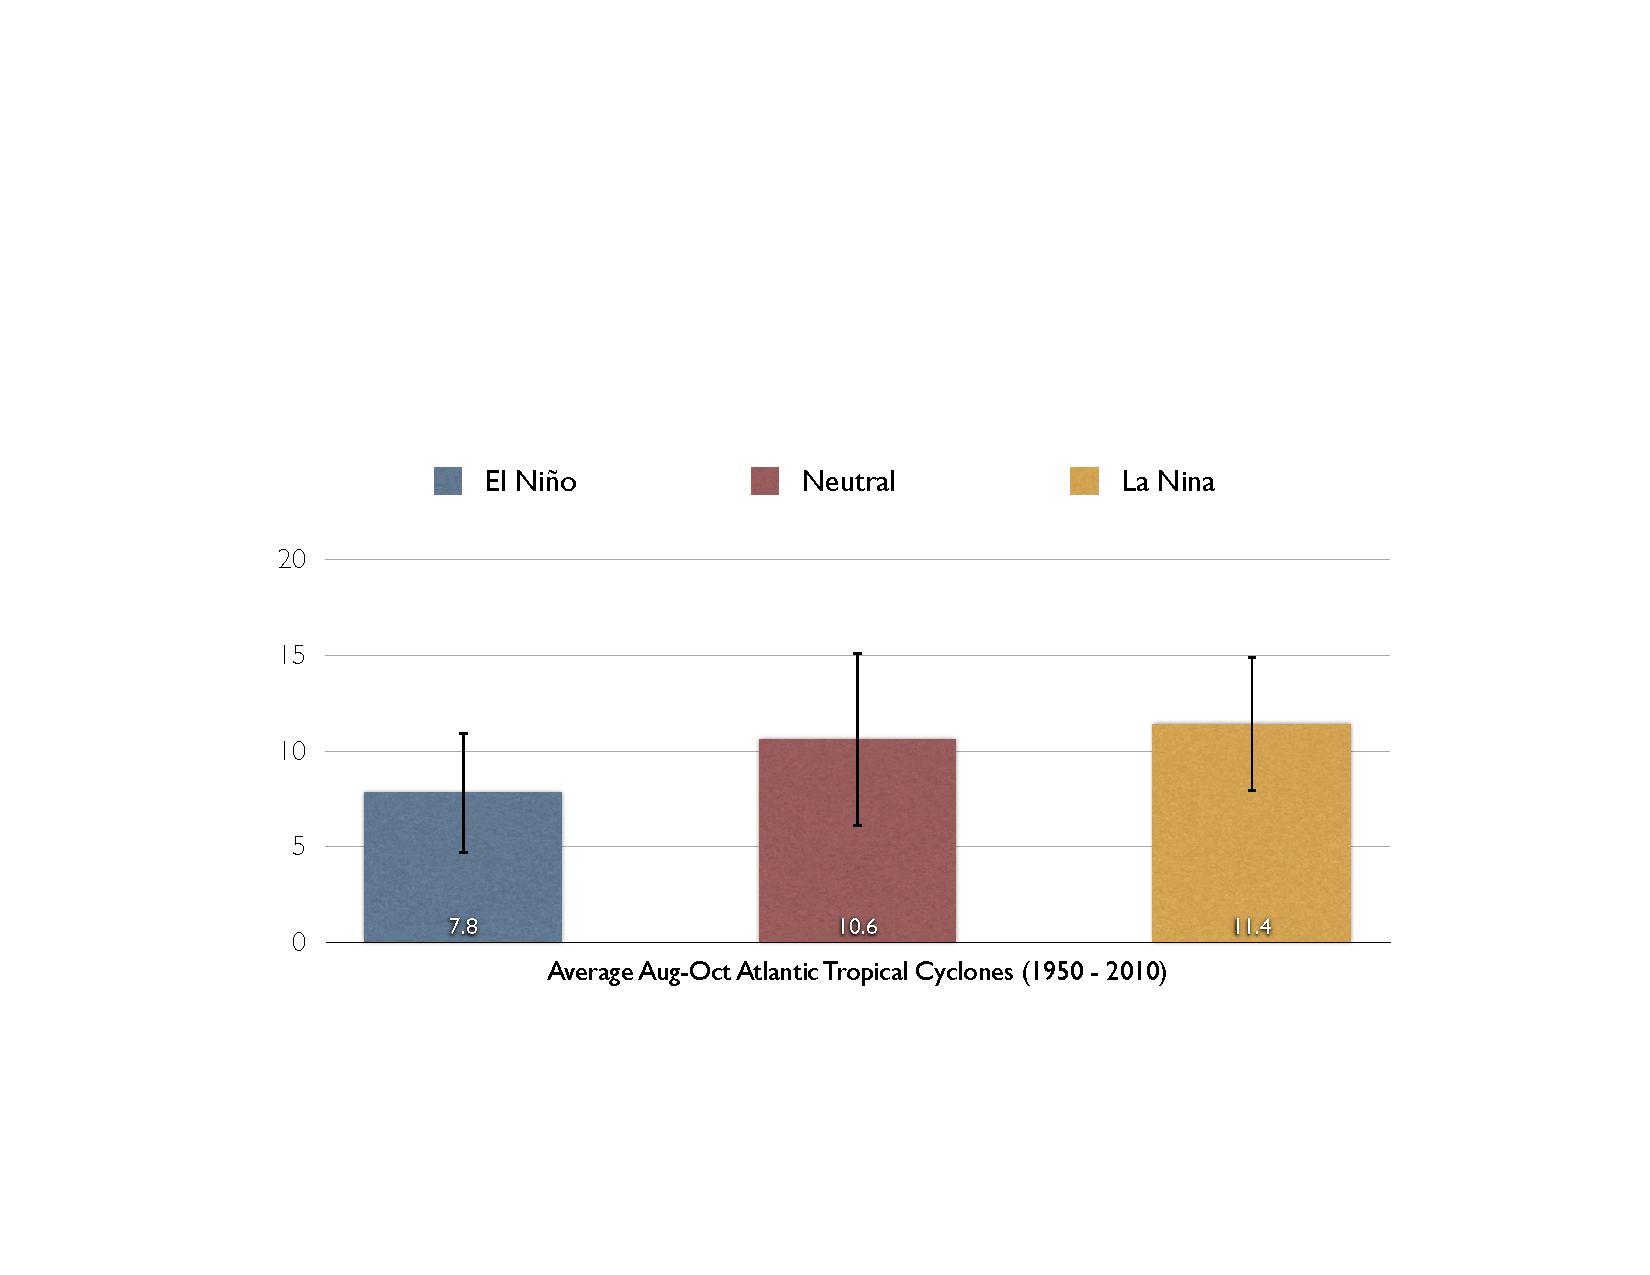
\includegraphics[height=3in]{figures/nino_tc_bars.pdf}
	\caption{The mean August-October Atlantic TC counts for Ni\~no (16 years), Neutral (39 years) and Ni\~na (10 years). The ENSO phases are based on NINO3.4 from 1950-2010. Error bars denote one standard deviation. This figure shows that while there are notable differences in TC counts based on the phase of ENSO, the large variability of TC counts make discerning ENSO's impact uncertain. The NINO3.4 index was built using ERSSTV3. TC counts are from the Unisys best track archive. See methods for full details.}
	\label{fig:figures_nino_tc_bars}
\end{figure}

Given that ENSO affects the large-scale conditions over the Atlantic through anomalous warming and its associated wind shear, it is not only important to monitor the intensity of warming along the equatorial Pacific -- something traditional NINO indices do -- but also to capture the location of the warming. We propose a distance-based ENSO index (S-ENSO for spatial ENSO) that tracks the longitude of highest SST anomaly in the tropical Pacific. We demonstrate its robustness in predicting seasonal Atlantic TC activity as well as resolving the large-scale conditions over the Atlantic. Such an index, coupled with other seasonal prediction methods based on Atlantic variables may prove to be a significant addition to dynamical and statistical TC forecast models.

\newpage

% 

%an increasing number of studies report a shifting in the spatial warming patterns of the Pacific therefore making the monitoring of fixed regions less informative (see Figure 1). 


%A common pathway by which Pacific SST warming affects the globe is through the alteration of the Walker circulation due to ---. 


%are Pacific sea surface temperatures (SST). Traditionally, Pacific SST's impact of the Atlantic has been abstracted by monitoring the warming of fixed oceanic regions (e.g. NINO3.4). However increasing evidence is suggesting that the spatio-temporal context of the warming must be considered (relative SST, NINO Modoki, etc.)

%We propose a new index that accounts for the spatial distribution of warming of Pacific SSTs and are able to explain 60\% of the seasonal variability in Atlantic TC frequency. The index is able to resolve the large-scale conditions during the Atlantic hurricane season better than warming-based indices. Such an index, coupled with other seasonal prediction methods based on Atlantic variables (e.g. Kneuston et al 2007, Emanuel et al 2008) can prove to be a significant addition to dynamical and statistical forecast models.

%A second approach to the problem is to use statistical relationships between tropical cyclones and large-scale predictors to estimate tropical cyclone activity as a function of variables that are resolved by climate models (e.g., Camargo et al. 2007a,b). One potential drawback of this approach is that the statistics are trained largely on natural variability, much of which is regional; it is not clear that such indices will perform well when applied to global climate change

% Pacific Ocean sea surface temperatures (SSTs) have well documented global long-range teleconnections, including Atlantic tropical cyclone (TC) activity \cite{gray1984a, bove1998,elsner2001b, emanuel2008, klotzbach2011nino}. The quasi-periodic cycle (2-7 years) of warming and cooling of the near equatorial Pacific Ocean, known as the El-Ni\~no Southern Oscillation (ENSO), has been used to predict Atlantic TC activity for decades. However, due to the large amplitude variations in seasonal TC counts, the difference in Atlantic TC activity based on the phase of ENSO is not obvious (see Figure \ref{fig:enso_bars}).
% 
% Traditionally, ENSO has been quantified using warming-based indices where SST anomalies are averaged over fixed regions in the Pacific Ocean. An increasing number of studies suggest that monitoring static regions may not be enough to capture the complex ENSO phenomenon \cite{trenberth2001, ashok2007,yeh2009,kim2009}. Furthermore, other studies proposed that the Pacific Ocean warming patterns are changing - with warm anomalies shifting towards the Central Pacific. Such changes have been attributed to anthropogenic global warming \cite{yeh2009} as well as natural climate variability \cite{wittenberg2009}. Based on these findings, it is evident that in order to capture ENSO's long range impact on the tropical Atlantic a new measure of Pacific warming is needed. 
% 
% 
% 
% We propose a novel spatial ENSO index (S-ENSO) that is designed specifically to capture the physical pathways by which Pacific SSTs may influence Atlantic TC activity. Tropical Atlantic SST variability west of 40W and extending into the Caribbean is correlated with Pacific ENSO variability, with 50-80\% of the anomalous SST variability in the region associated with ENSO \cite{enfield97}. However, a large number of TCs, especially the most intense hurricanes, originate east of 40W (based on the NOAA best track hurricane data). Therefore, it is important for any index to resolve the large-scale conditions over the eastern tropical Atlantic. Our approach introduces a distance-based ENSO index that tracks the location of maximum near-tropical Pacific warming anomaly instead of its absolute warming. We will demonstrate the performance of our index by comparing it to traditional warming-based ENSO indices in discriminating between the large-scale conditions that are favorable for Atlantic cyclogenesis.

\section{Shifting of ENSO}
Given the increasing number of studies reporting a shift in ENSO's warming patterns \cite{ashok2007, kao2009contrasting, yeh2009,kug2009two, kim2009}, we examine empirically the extent of such a shift. For every month from January 1979 to November 2012, we monitor the longitude of the warmest $10^\circ$ latitude by $40^\circ$ longitude region in the Pacific (see methods for details). As it can be seen in Figure \ref{fig:figures_scatter} there has been a distinct westward shift in the longitude of the warmest Pacific region. This may explain how traditional NINO indices were initially successful in abstracting the impact Pacific warming might have on Atlantic TCs, but as the warming gradually shifted westward they have grown less accurate.

\begin{figure}[htbp]
	\centering
		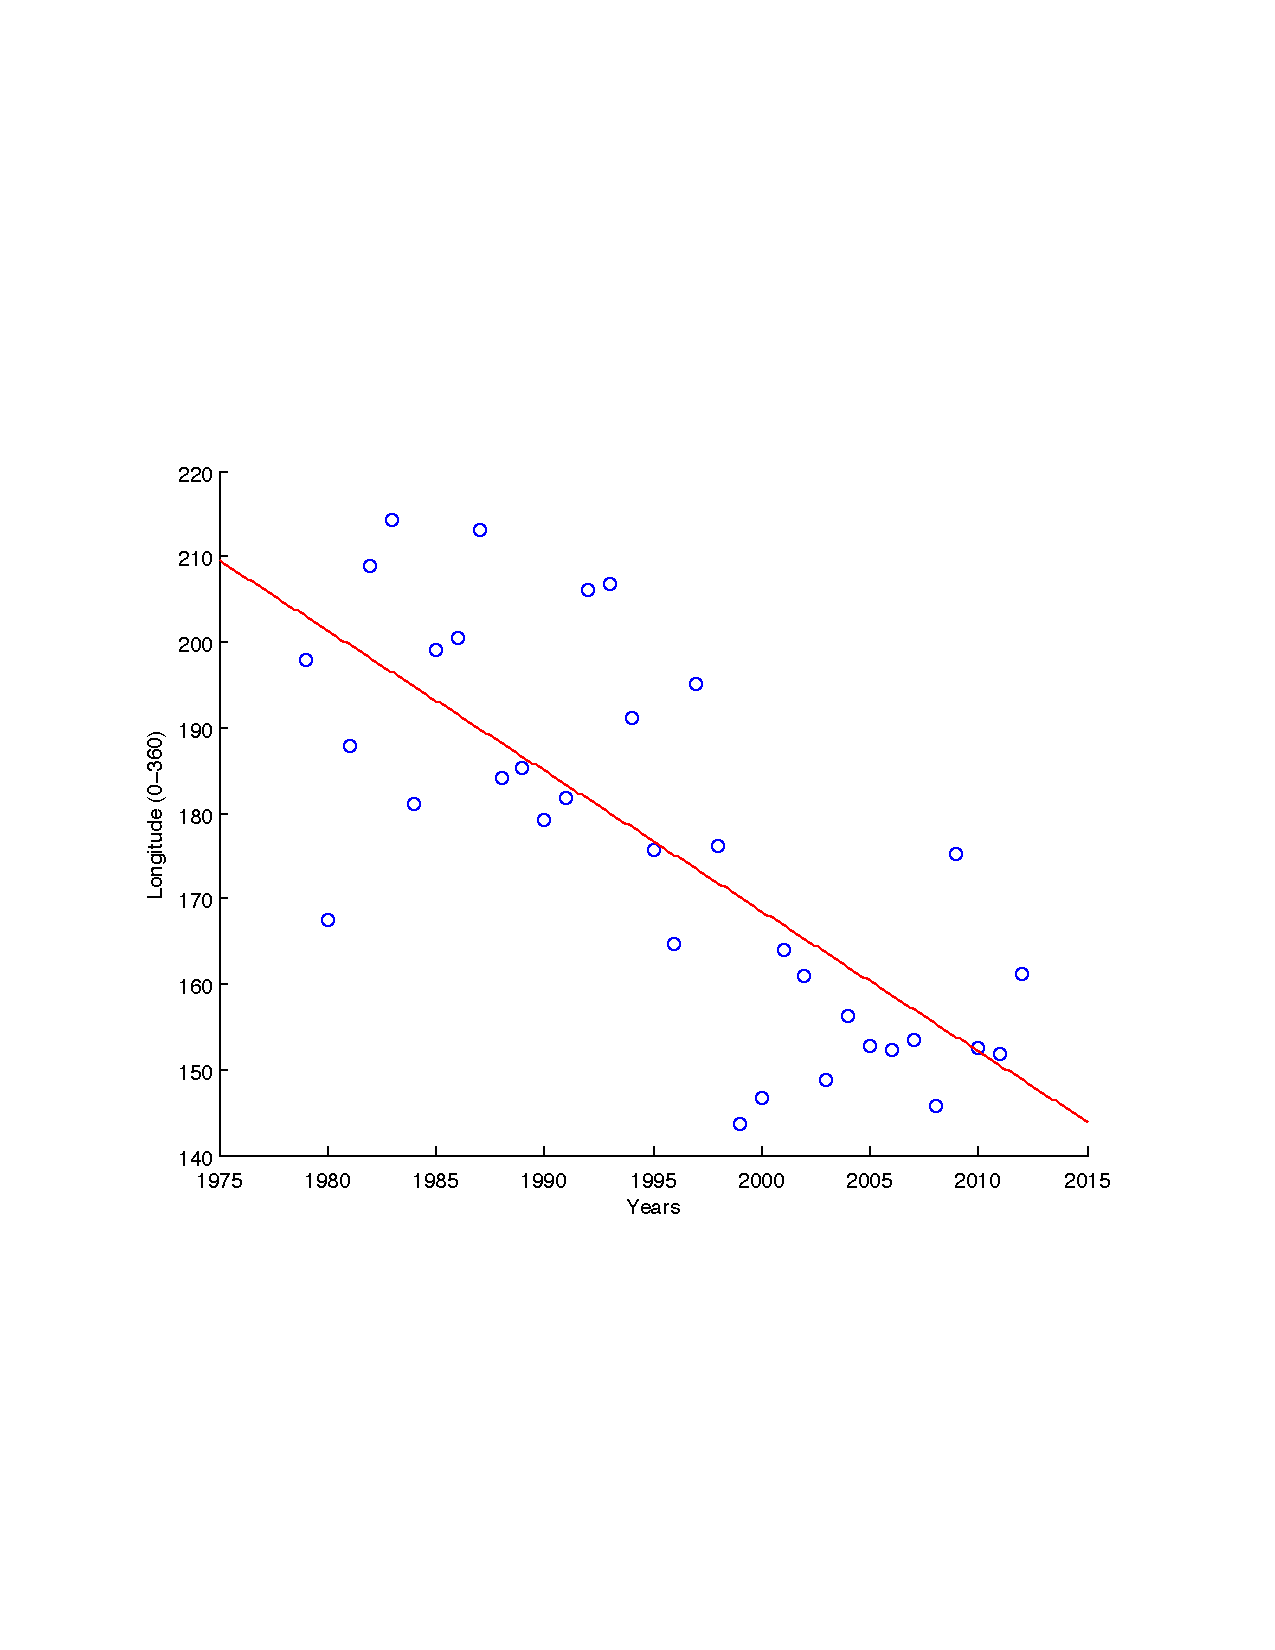
\includegraphics[height=3in]{figures/scatter.pdf}
	\caption{The annual mean longitude of the warmest SST anomaly region in the Pacific ($1979-2012$). The figure shows a clear westward shift the warmest region in the Pacific. $R^2 = 0.54$ $p < 0.01$}
	\label{fig:figures_scatter}
\end{figure}

%This westward shift might explain traditional NINO indices' lack of accuracy. Earlier in the record, the warmest region in the Pacific might have coincided with the region's these static indices monitor, but as the warming began to shift westward the accuracy of such static indices began to deteriorate. 

\newpage
\section{S-ENSO an index for a shifting warming patters}
We propose that the spatial distribution of Pacific Ocean warming might provide better predictive insights into ENSO-Atlantic TC activity relationship than warming anomalies alone. For this analysis we use June-October S-ENSO index (see methods). Table \ref{ref:lin_corr} shows S-ENSO's linear correlation coefficients with various quantities that communicate August-October Atlantic TC activity: number of tropical cyclones, number of major hurricanes, potential dissipation index (PDI) \cite{emanuel2005a}, accumulated cyclone energy (ACE) \cite{Bell2000}, and net tropical cyclone energy (NTC) \cite{goldenberg2001}. The significant improvement over traditional static NINO indices, especially with regards to cumulative statistics such as ACE and NTC, indicates that S-ENSO resolves the large-scale conditions over the Atlantic as well as the in-season TC precursors than traditional more accurately than static warming-base indices.

\begin{table}
\begin{tabular}{cccccc}
\hline
&TCs & Major Hurricanes & NTC & PDI & ACE\\
\hline
%S-ENSO  & \textbf{0.81} & \textbf{0.81} & \textbf{0.77} & \textbf{0.71} & \textbf{0.75}\\
%PWP-Pres & 0.61 & 0.65 & 0.57 & 0.56 & 0.58\\
%PWP-OLR & 0.55 & 0.57 & 0.50 & 0.46 & 0.48\\
%MinPres-Lon & 0.15 & 0.12 & 0.19 & 0.17 & 0.20\\
%PWP-PCP  & 0.67 & 0.66 & 0.64 & 0.6 & 0.58\\
%maxSSTALon & \textbf{-0.64} & -0.5 & \textbf{-0.55} & -0.44 & \textbf{-0.49}\\
S-ENSO & \textbf{-0.75} & \textbf{-0.59} &\textbf{-0.74} & \textbf{-0.68} & \textbf{-0.73}\\
Nino1+2 & -0.51 & -0.46 & -0.46 & -0.4 & -0.42\\
Nino 3 & -0.51 & -0.51 & -0.48 & -0.44 & -0.45\\
Nino 4 & -0.32 & -0.47 & -0.32 & -0.3 & -0.31\\
Nino 3.4 & -0.47 & -0.53 & -0.46 & -0.43 & -0.45\\
%Modoki Box A & -0.28 & -0 & -0.26 & -0.24 & -0.3\\
%Modoki Box B & -0.41 & -0.40 & -0.4 & -0 & -0.33\\
%Modoki Box C & 0.55 & 0.57 & 0.57 & 0.57 & 0.59\\
%Modoki EMI & -0.062 & -0.21 & -0.088 & -0.11 & -0.12\\
\hline
\end{tabular}
\caption{Linear correlation coefficients between the June-October S-ENSO and August-October Atlantic TC activity. The highest score for each category is highlighted in \textbf{bold}. All correlations are significant at $95\%$ level}
\label{ref:lin_corr}
\end{table}

In addition to providing increased in-season accuracy than traditional NINO indices, S-ENSO is more robust to the ENSO spring predictability barrier \cite{webster1992}. Figure \ref{fig:figures_lead_time_bar} shows the performance of each NINO index as well as S-ENSO as a function of lead time. While S-ENSO's performance drops with January lead time, it is nearly an order of magnitude stronger than that of some static NINO indices. In fact, give the 30 degrees of freedom in the data (N=32; df = N-2), the traditional NINO indices do not provide significant correlations until July as opposed to March for S-ENSO. Furthermore, the improved accuracy remains significant from January until October. Therefore, if dynamical models can resolve the spatial patterns of ENSO as represented by S-ENSO then dynamical models could potentially have significant skill in predicting August-October TC activity.

\begin{figure}[htbp]
	\centering
		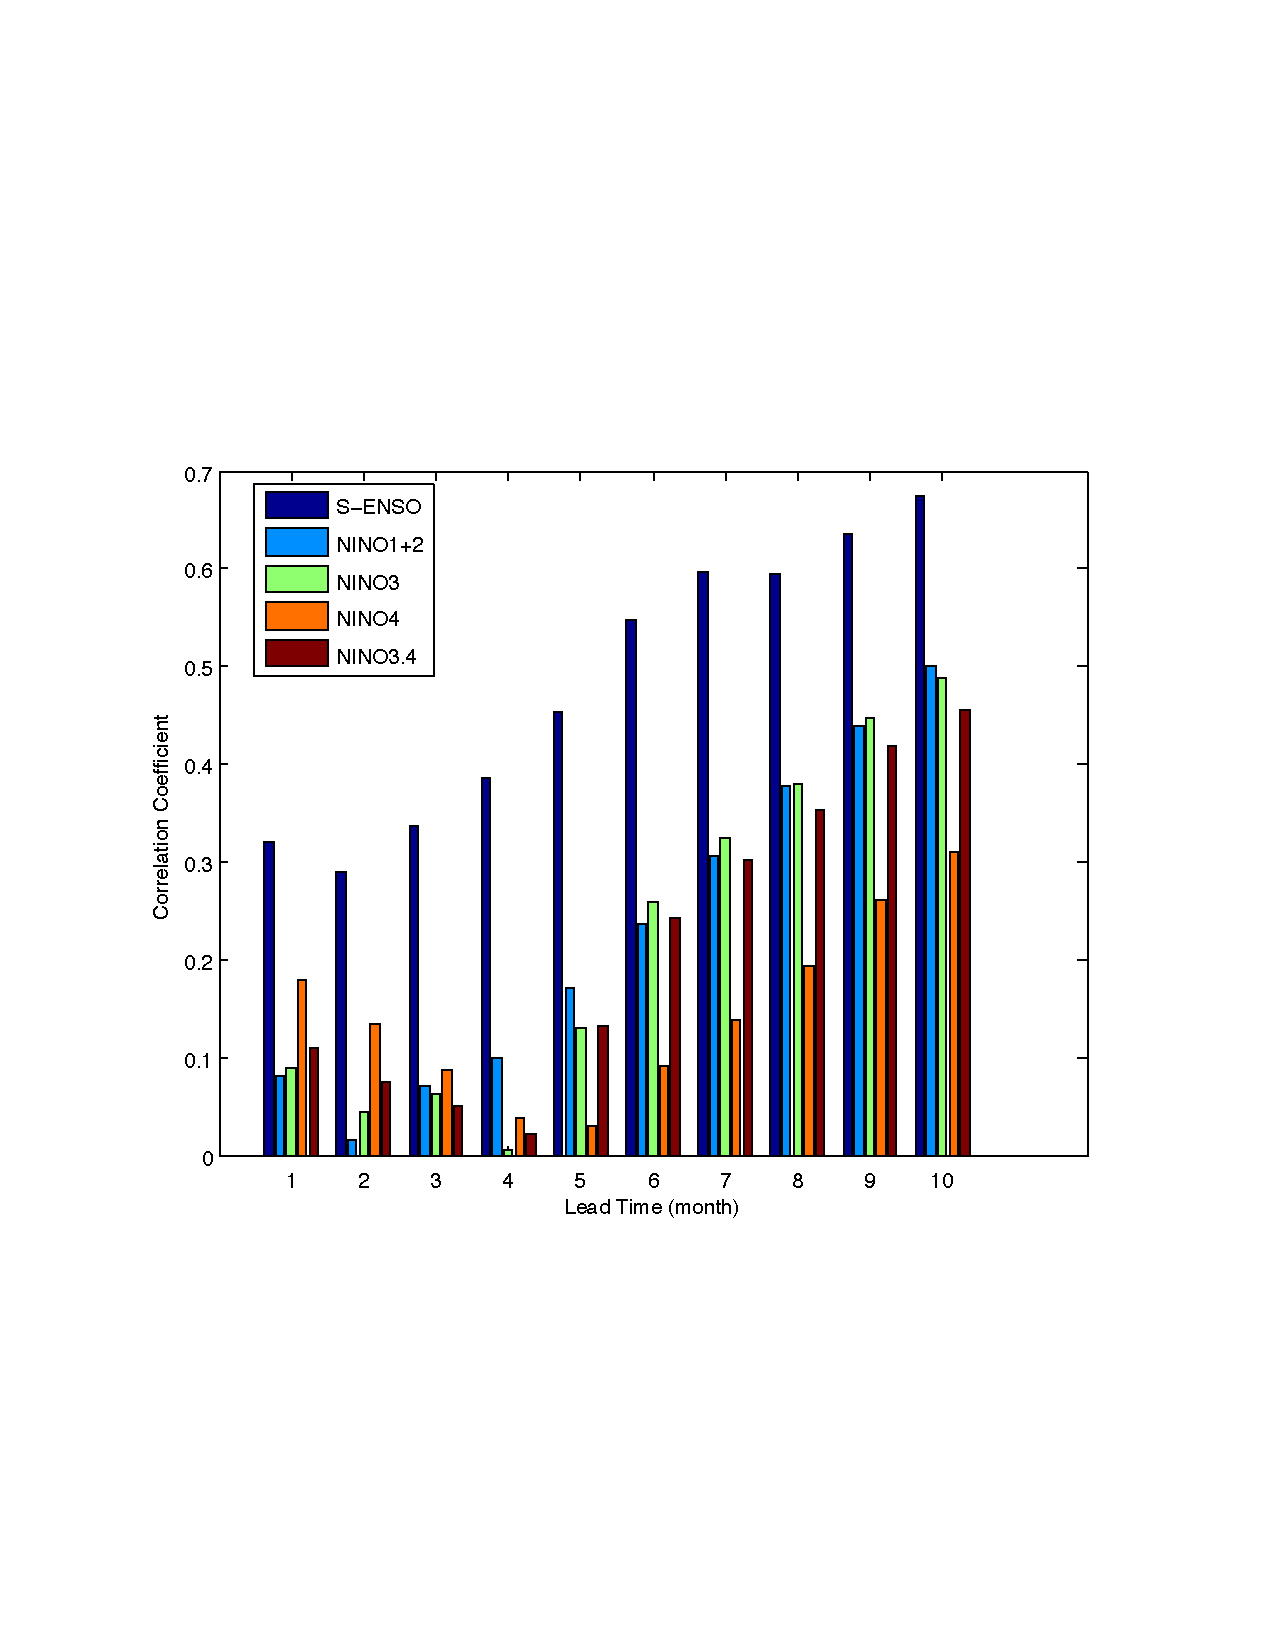
\includegraphics[height=3in]{figures/lead_time_bar.pdf}
	\caption{The linear correlation coefficients between different ENSO indices and Atlantic August-October TC counts. The x-axis denotes the last month used to build each index (see methods). The indices increase in accuracy as we move closer to the TC season, however S-ENSO performance is not as severely affected by the ENSO predictability barrier as traditional NINO indices.}
	\label{fig:figures_lead_time_bar}
\end{figure}

\newpage

%\section{S-ENSO's impact on large-scale conditions over the Atlantic}
To propose possible physical pathways by which our index impact Atlantic TC activity, we compute the composites for factors known to influence Atlantic TC activity: potential intensity (PI), vertical wind shear between 850 and 200 hPa, and SST. Each composite was for the August-October period - the peak hurricane season. To compare how well our index resolves the large-scale conditions that are critical to seasonal TC activity we compare our index' composites to those of the seasonal TC count composites (baseline) and those of the most common warming-based ENSO index: NINO3.4. The idea is that if our index is better able to distinguish between the large-scale conditions for active and inactive hurricane seasons its composites should closely resemble those of the baseline (i.e. active minus inactive hurricane years). Furthermore, Recent hurricane downscaling studies \cite{knutson2007simulation, emanuel2010comparison} as well as genesis indices \cite{menkes2012comparison} have shown that the large scale environment over the Atlantic might play a dominant role in modulating Atlantic TC activity than precursor disturbances, since these simulations do not model such disturbances yet are able to reproduce Atlantic TC climatology with significant accuracy.

%Previous work investigating the ENSO-Atlantic TC teleconnection proposed that enhanced convection as a result of anomalous Pacific Ocean warming during the El Niño phase is associated with strong westerly upper tropospheric wind over the Caribbean basin and tropical Atlantic, resulting in low TC activity during ENSO's warm phase (El Ni\~{n}o) events and high TC activity during its cold phase (La Ni\~{n}a). Warm eastern Pacific SST and negative (drought) Sahelian rainfall anomalies are associated with suppressed Atlantic basin tropical cyclone activity through an equatorially confined near-zonal circulation with upper-level westerlies and lower-level easterlies that act to increase the climatological westerly vertical shear in the main development region \cite{goldenberg1996physical}. Other studies have suggested that ENSO impact Atlantic TC activity via tropospheric warming \cite{tang2004}, since warm free tropospheric temperatures that are spread eastward from the Pacific by equatorial wave dynamics (e.g. Kelvin waves) can inhibit TC activity by providing a too weak vertical temperature gradient for TC activity to occur. Analogous to reduced vertical temperature gradient, a reduced vertical gradient of saturation deficit suppresses vertical mixing and thus negatively affects TC activity.

However, it seems that by monitoring the deep convection associated with the region with the highest Pacific SST warming anomaly, we succeed to observe the strength and location of updrafts related to this convection and the resulting strength and location of the zonal Walker circulation, as well as its impact on the tropical Atlantic circulation, as described in e.g. \cite{liu2004remote}, who  suggest that the remote impact contributes to nearly half of the variance of the tropical Atlantic SST variability at interannual and decadal time scales. Updrafts over the eastern and central Pacific during El Ni\~no result in downdrafts and therefore reduced TC activity over the tropical Atlantic, whereas updrafts over the western Pacific during neutral and La Ni\~na years result in downdrafts over the eastern tropical Pacific and updrafts over the Atlantic, thus leading to increased TC activity.

\begin{figure}[htbp]

\hspace{-2.5cm}		
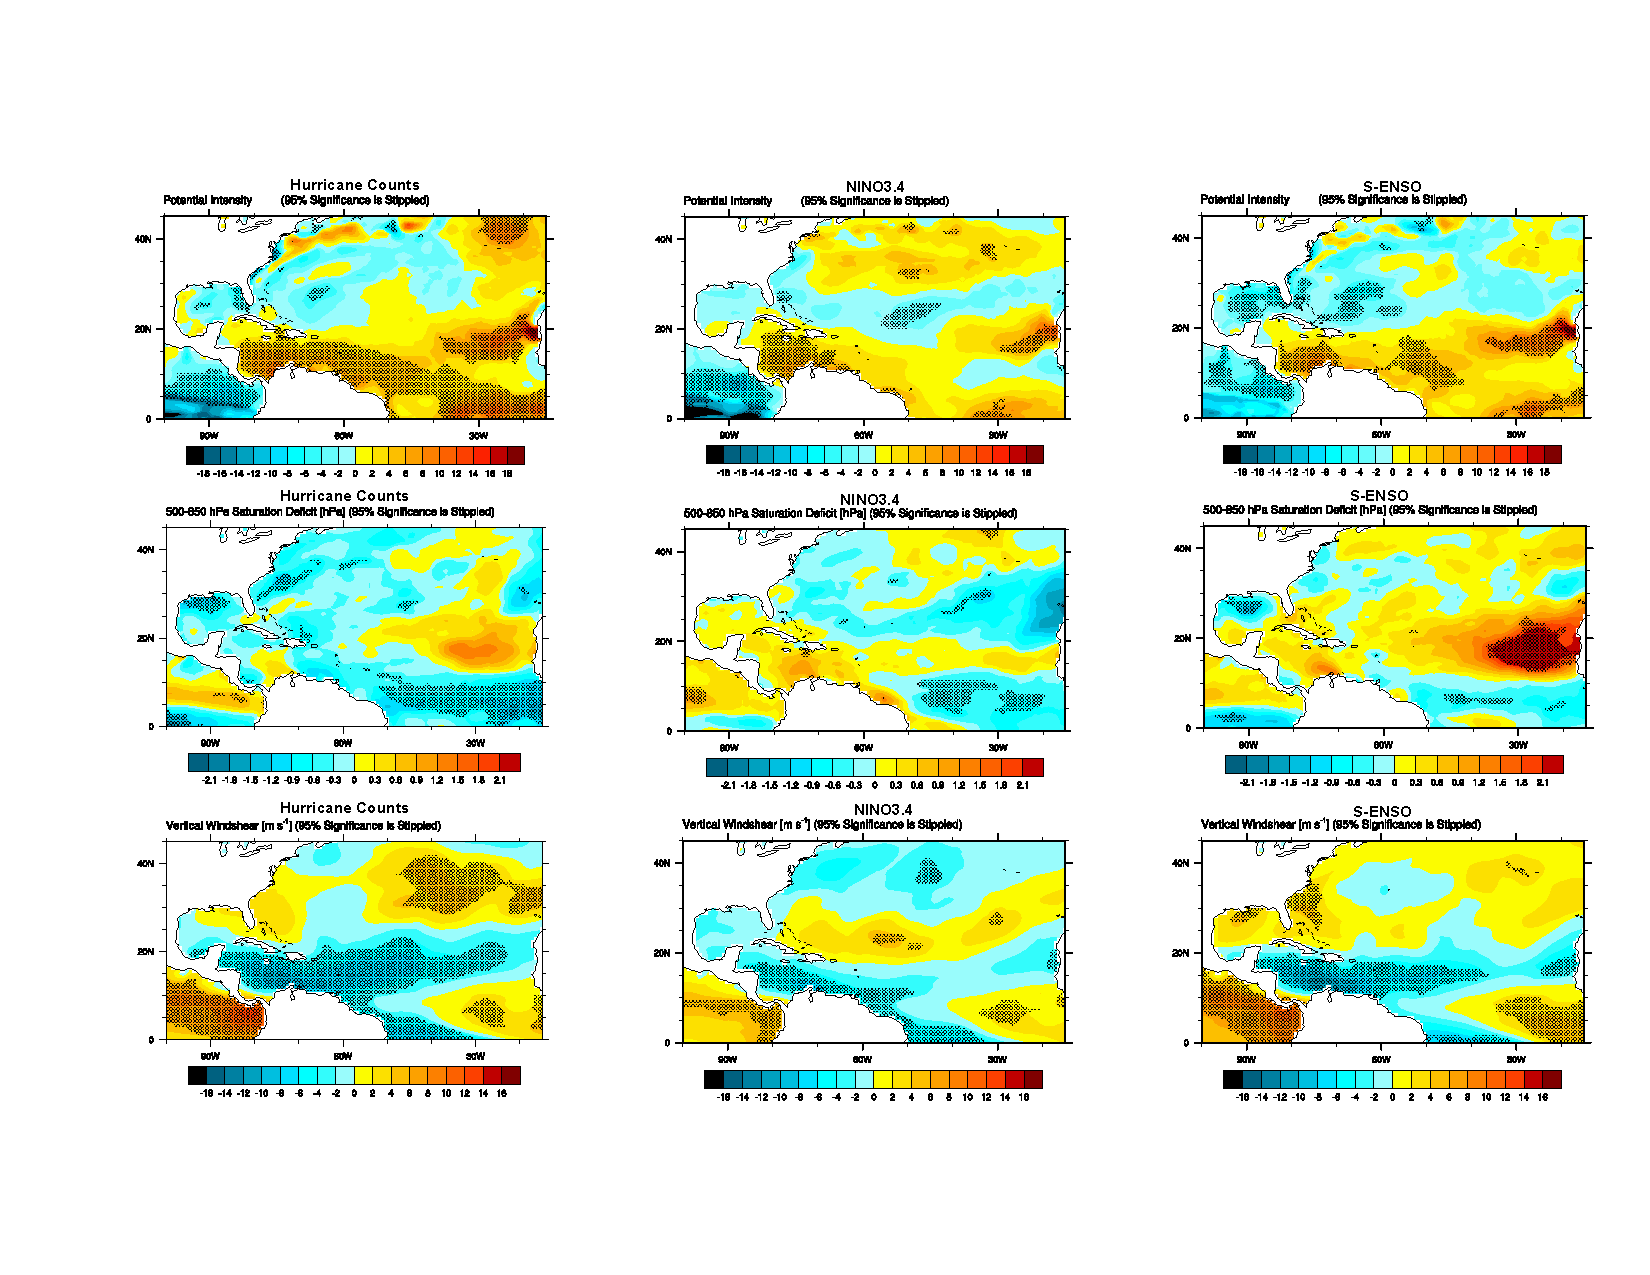
\includegraphics[width=7in]{figures/3_by_3_composites.pdf}
	\caption{composites for PI (top row), the difference in saturation deficit between 500 and 850 hPa (middle row), and vertical wind shear between 200 and 850 hPa (bottom) row. Each column shows the composites for hurricane counts (left), NINO3.4 (middle), and S-ENSO (right). $95\%$ significance intervals are shaded. Shaded area represents $95\%$ significance level. The hurricane count positive years (6) are: 1995, 2001, 2003, 2005, 2008, and 2010. The hurricane count negative years (8) are: 1982, 1983, 1986, 1987, 1992, 1993, 1994, 1997 and 2002. The NINO3.4 positive years (8) are: 1981, 1984, 1985, 1988, 1999, 2000, 2007, and 2008. The NINO3.4 negative years (6) are: 1982, 1987, 1991, 1992, 1997, 2002. S-ENSO positive years (6) are: 1989, 1995, 2003, 2005, 2008, 2010. S-ENSO negative years (6) are: 1982, 1983, 1991, 1997, 1998, 2002. For all three variables, S-ENSO reproduces the large scale environment over the Atlantic better than the traditional warming-based ENSO index NINO3.4}
	\label{fig:olr_comp}
\end{figure}
\section{Summary of Methods}
\subsection{S-ENSO}
The S-ENSO index is computed by first averaging the SST anomalies over the June-October period to accurately capture ENSO's evolution prior to and during the Atlantic hurricane season (August-October). We then search the tropical Pacific ($5^\circ$S-$30^\circ$N) for a region of similar size to traditional ENSO indices that has the highest mean SST anomaly over the June-October period. We repeat this procedure for each year from 1979 to 2010. Monthly SST anomalies we computed from the ERSSTV3 monthly SST dataset \cite{reynolds2002}. See Figure \ref{fig:s_enso_graphic}.

\begin{figure}[htbp]
	\centering
		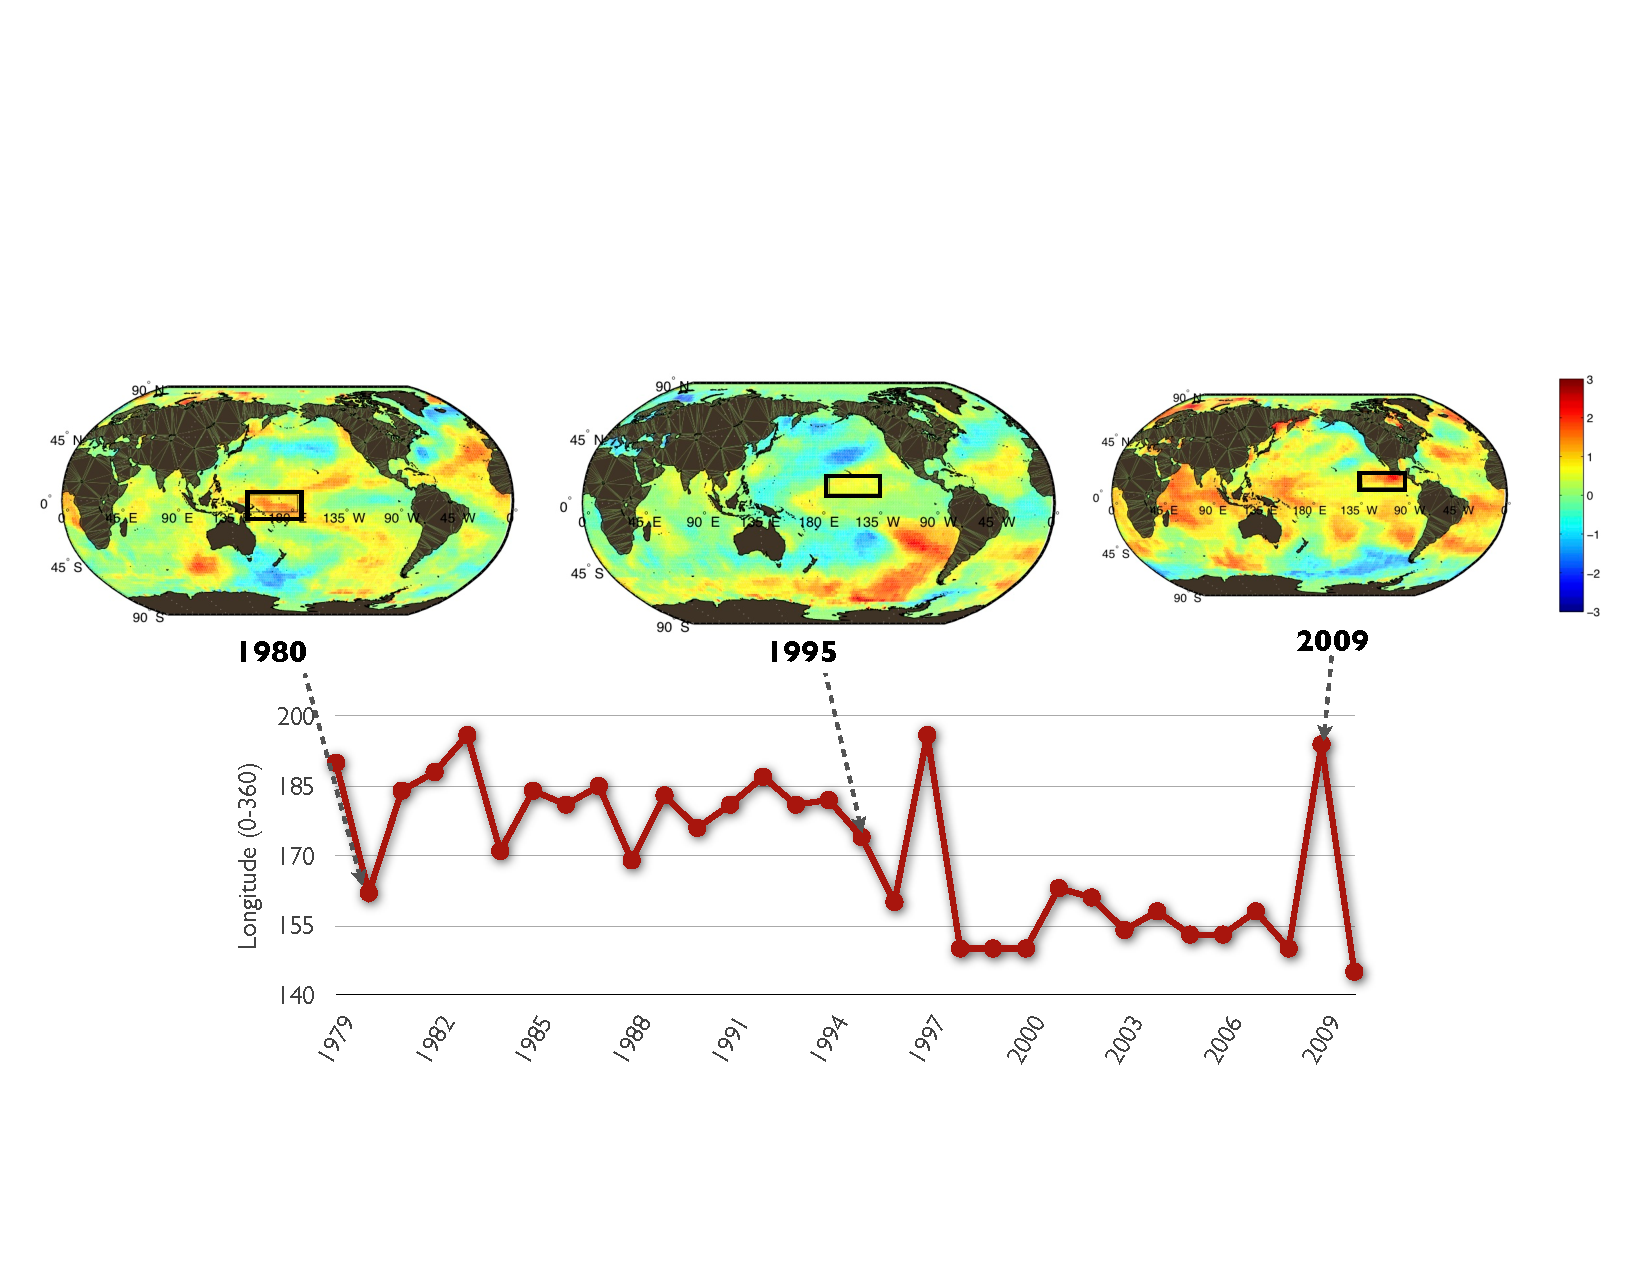
\includegraphics[width=5in]{figures/s_enso_graphic.pdf}
	\caption{A schematic demonstrating how the S-ENSO index is built. First, SST anomalies over a certain month range are computed resulting in maps similar to those above. Next, we search the tropical Pacific for the region with the highest mean SST warming anomaly. Finally, we record the longitude of that region. We repeat this procedure for all years from 1979-2010. }
	\label{fig:s_enso_graphic}
\end{figure}

\subsection{Lead Times Analysis}
Figure \ref{fig:figures_lead_time_bar} shows the relative ability of each index to forecast Atlantic TC activity as a function of lead time. Each index (S-ENSO, NINO1.2, \emph{etc.}) is computed by first averaging SST anomalies over a certain month range denoted by a start and end month. The resulting index is then correlated with August-October Atlantic TC counts. For each month on the x-axis, we average the performance of all variations of the indices that end in the month indicated on the chart (end month varies from January to October). 
For example, the first set of bars were obtained by averaging the performance of all indices end month was January. In this case, there is only one such index the January-January index. The values for the June lead month (number 6 on the x-axis) were obtained by averaging the performance of all indices that had a June end month. There are 6 such indices: January-June, February-June, March-June, April-June, May-June, and June-June. This procedure was repeated for all indices and end months ranging from January to October.

%\subsection{Large-scale composites}
%To compare the large-scale conditions over the Atlantic during active and inactive TC seasons we compute the composites of potential intensity (PI) , saturation deficit, and vertical wind shear -- all elements critical for TC activity. 


\newpage

\section{Future Work}
\subsection{Increased seasonal predictability through monitoring the SST warming patterns and associated impact}
In addition to monitoring the location of the largest warming anomaly in the Pacific, we have also monitored the resulting deep convection and other spatial patterns such as the mean SST empirical orthogonal function (EOF). A combination of such quantities may yield a significant improvement over the state-of-the-art statistical forecasting algorithms.

\section{Monitoring the spatial warming patterns in the Pacific allows us to by-pass the ENSO predictability barrier}
While S-ENSO is more robust than tradition NINO indices to increased lead times, we are investigating how predictable such spatial patterns are. If we are able to predict the warming distribution several months in advance, then that would be a significant contribution to TC forecasting techniques. We also plan on investigating whether current SST forecast models such as ECMWF are able to reproduce S-ENSO.

\section{Monitoring the spatial distribution of the warmest and coldest SST anomaly regions in the Pacific encapsulates the Pacific SST EOF}
We also built an index that monitors the distance between the coldest and warmest SST region in the Pacific, which is similar to what the EOF does in terms of looking at extremes to explain variability. Such an analysis allows for a more detailed monitoring of ENSO's evolution. Our preliminary analysis shows that both the spatial distribution and the EOF's first principal component explain the same amount of TC variability.
%\section{Claim 1: Monitoring the spatial warming patterns of the Tropical Pacific Ocean provides better insight on the Pacific's impact on Atlantic tropical cyclone (TC) frequency than warming-based indices}
%%
%  claim2
%
%  Created by James on 2012-12-07.
%  Copyright (c) 2012 __MyCompanyName__. All rights reserved.
%
\documentclass[]{article}

% Use utf-8 encoding for foreign characters
\usepackage[utf8]{inputenc}

% Setup for fullpage use
\usepackage{fullpage}

% Uncomment some of the following if you use the features
%
% Running Headers and footers
%\usepackage{fancyhdr}

% Multipart figures
%\usepackage{subfigure}

% More symbols
%\usepackage{amsmath}
%\usepackage{amssymb}
%\usepackage{latexsym}

% Surround parts of graphics with box
\usepackage{boxedminipage}

% Package for including code in the document
\usepackage{listings}

% If you want to generate a toc for each chapter (use with book)
\usepackage{minitoc}

% This is now the recommended way for checking for PDFLaTeX:
\usepackage{ifpdf}

%\newif\ifpdf
%\ifx\pdfoutput\undefined
%\pdffalse % we are not running PDFLaTeX
%\else
%\pdfoutput=1 % we are running PDFLaTeX
%\pdftrue
%\fi

\ifpdf
\usepackage[pdftex]{graphicx}
\else
\usepackage{graphicx}
\fi
\title{A LaTeX Article}
\author{  }

\date{2012-12-07}

\begin{document}

\ifpdf
\DeclareGraphicsExtensions{.pdf, .jpg, .tif}
\else
\DeclareGraphicsExtensions{.eps, .jpg}
\fi

\maketitle


\begin{abstract}
\end{abstract}

\section{Introduction}

\bibliographystyle{plain}
\bibliography{}
\end{document}

%%
%  claim3
%
%  Created by James on 2012-12-07.
%  Copyright (c) 2012 __MyCompanyName__. All rights reserved.
%
\documentclass[]{article}

% Use utf-8 encoding for foreign characters
\usepackage[utf8]{inputenc}

% Setup for fullpage use
\usepackage{fullpage}

% Uncomment some of the following if you use the features
%
% Running Headers and footers
%\usepackage{fancyhdr}

% Multipart figures
%\usepackage{subfigure}

% More symbols
%\usepackage{amsmath}
%\usepackage{amssymb}
%\usepackage{latexsym}

% Surround parts of graphics with box
\usepackage{boxedminipage}

% Package for including code in the document
\usepackage{listings}

% If you want to generate a toc for each chapter (use with book)
\usepackage{minitoc}

% This is now the recommended way for checking for PDFLaTeX:
\usepackage{ifpdf}

%\newif\ifpdf
%\ifx\pdfoutput\undefined
%\pdffalse % we are not running PDFLaTeX
%\else
%\pdfoutput=1 % we are running PDFLaTeX
%\pdftrue
%\fi

\ifpdf
\usepackage[pdftex]{graphicx}
\else
\usepackage{graphicx}
\fi
\title{A LaTeX Article}
\author{  }

\date{2012-12-07}

\begin{document}

\ifpdf
\DeclareGraphicsExtensions{.pdf, .jpg, .tif}
\else
\DeclareGraphicsExtensions{.eps, .jpg}
\fi

\maketitle


\begin{abstract}
\end{abstract}

\section{Introduction}

\bibliographystyle{plain}
\bibliography{}
\end{document}






%%%%%%%%%%%%%%%%%%%%%%%%%

\begin{comment}
\section{Introduction}
Pacific Ocean sea surface temperatures (SSTs) have well documented global long-range teleconnections, including Atlantic tropical cyclone (TC) activity \cite{gray1984a, bove1998,elsner2001b, emanuel2008, klotzbach2011nino}. The quasi-periodic cycle (2-7 years) of warming and cooling of the near equatorial Pacific Ocean, known as the El-Ni\~no Southern Oscillation (ENSO), has been used to predict Atlantic TC activity for decades. However, due to the large amplitude variations in seasonal TC counts, the difference in Atlantic TC activity based on the phase of ENSO is not obvious (see Figure \ref{fig:enso_bars}).

Traditionally, ENSO has been quantified using warming-based indices where SST anomalies are averaged over fixed regions in the Pacific Ocean. An increasing number of studies suggest that monitoring static regions may not be enough to capture the complex ENSO phenomenon \cite{trenberth2001, ashok2007,yeh2009,kim2009}. Furthermore, other studies proposed that the Pacific Ocean warming patterns are changing - with warm anomalies shifting towards the Central Pacific. Such changes have been attributed to anthropogenic global warming \cite{yeh2009} as well as natural climate variability \cite{wittenberg2009}. Based on these findings, it is evident that in order to capture ENSO's long range impact on the tropical Atlantic a new measure of Pacific warming is needed. 



We propose a novel spatial ENSO index (S-ENSO) that is designed specifically to capture the physical pathways by which Pacific SSTs may influence Atlantic TC activity. Tropical Atlantic SST variability west of 40W and extending into the Caribbean is correlated with Pacific ENSO variability, with 50-80\% of the anomalous SST variability in the region associated with ENSO \cite{enfield97}. However, a large number of TCs, especially the most intense hurricanes, originate east of 40W (based on the NOAA best track hurricane data). Therefore, it is important for any index to resolve the large-scale conditions over the eastern tropical Atlantic. Our approach introduces a distance-based ENSO index that tracks the location of maximum near-tropical Pacific warming anomaly instead of its absolute warming. We will demonstrate the performance of our index by comparing it to traditional warming-based ENSO indices in discriminating between the large-scale conditions that are favorable for Atlantic cyclogenesis. 


%The influence of ENSO in the prediction skill over the tropical Atlantic is also consistent with the ENSO teleconnection over the tropical Atlantic in both observations and model simulations \cite{hu12}. However, the ENSO phenomenon is more complex than can be explained by a locally fixed index \cite{kim2009}, and TC activity can be influenced by other remote SST changes \cite{vecchi2007effect}.

%It has been proposed that enhanced convection as a result of anomalous Pacific Ocean warming is associated with strong westerly upper tropospheric wind over the Caribbean basin and tropical Atlantic, resulting in low TC activity during ENSO's warm phase and high TC activity during its cold phase \cite{gray1984}. Other studies have suggested that ENSO impacts Atlantic TC activity via tropospheric warming \cite{tang2004}.




%Given its long-range teleconnections, as well as ENSO being the most dominant feature of cyclic climate variability on subdecadal timescales, effectively abstracting and predicting Pacific Ocean warming anomalies has been a subject of active research.




%Such indices include the Nino 1+2 (0-10S, 90-80W), Nino 3 (5N-5S, 150-90W), Nino 4 (5N-5S, 160E-150W), and Nino 3.4 (5N-5S, 170-120W) regions. Some studies have suggested such indices do not capture ENSO's nature and evolution. Subsequently, more elaborate indices were developed some of which were linear combinations of the above-mentioned indices \cite{trenberth2001}, while others have proposed indices using transformed data or nonlinear combination of indices \cite{ren2011}. Despite the varying degrees of complexity, the majority of works attempting to capture ENSO focus on the intensity of warming in a the tropical Pacific. While such indices might provide valuable insight into weather teleconnections, they were not designed to capture the physical pathways by which Pacific SSTs may impact the large-scale conditions over the Atlantic. Recent hurricane downscaling studies \cite{knutson2007simulation, emanuel2010comparison} as well as genesis indices \cite{menkes2012comparison} have shown that the large scale environment over the Atlantic might play a dominant role in modulating Atlantic TC activity than precursor disturbances, since these simulations do not model such disturbances yet are able to reproduce Atlantic TC climatology with significant accuracy. Therefore, increasing our ability to predict the large-scale environment over the Atlantic could have significant scientific and societal value.



%One of the ENSO teleconnections is with North Atlantic tropical cyclone (TC) activity. The influence of ENSO on Atlantic TCs is well documented \cite{gray1984a, bove1998, elsner2001b,klotzbach2011nino}, however due to the large amplitude variations of seasonal counts, the difference in Atlantic TC activity based on the various phases of ENSO is not obvious (see Figure \ref{fig:enso_bars}).

\begin{figure}[htbp]
	\hspace*{-.5cm}
	\centering
		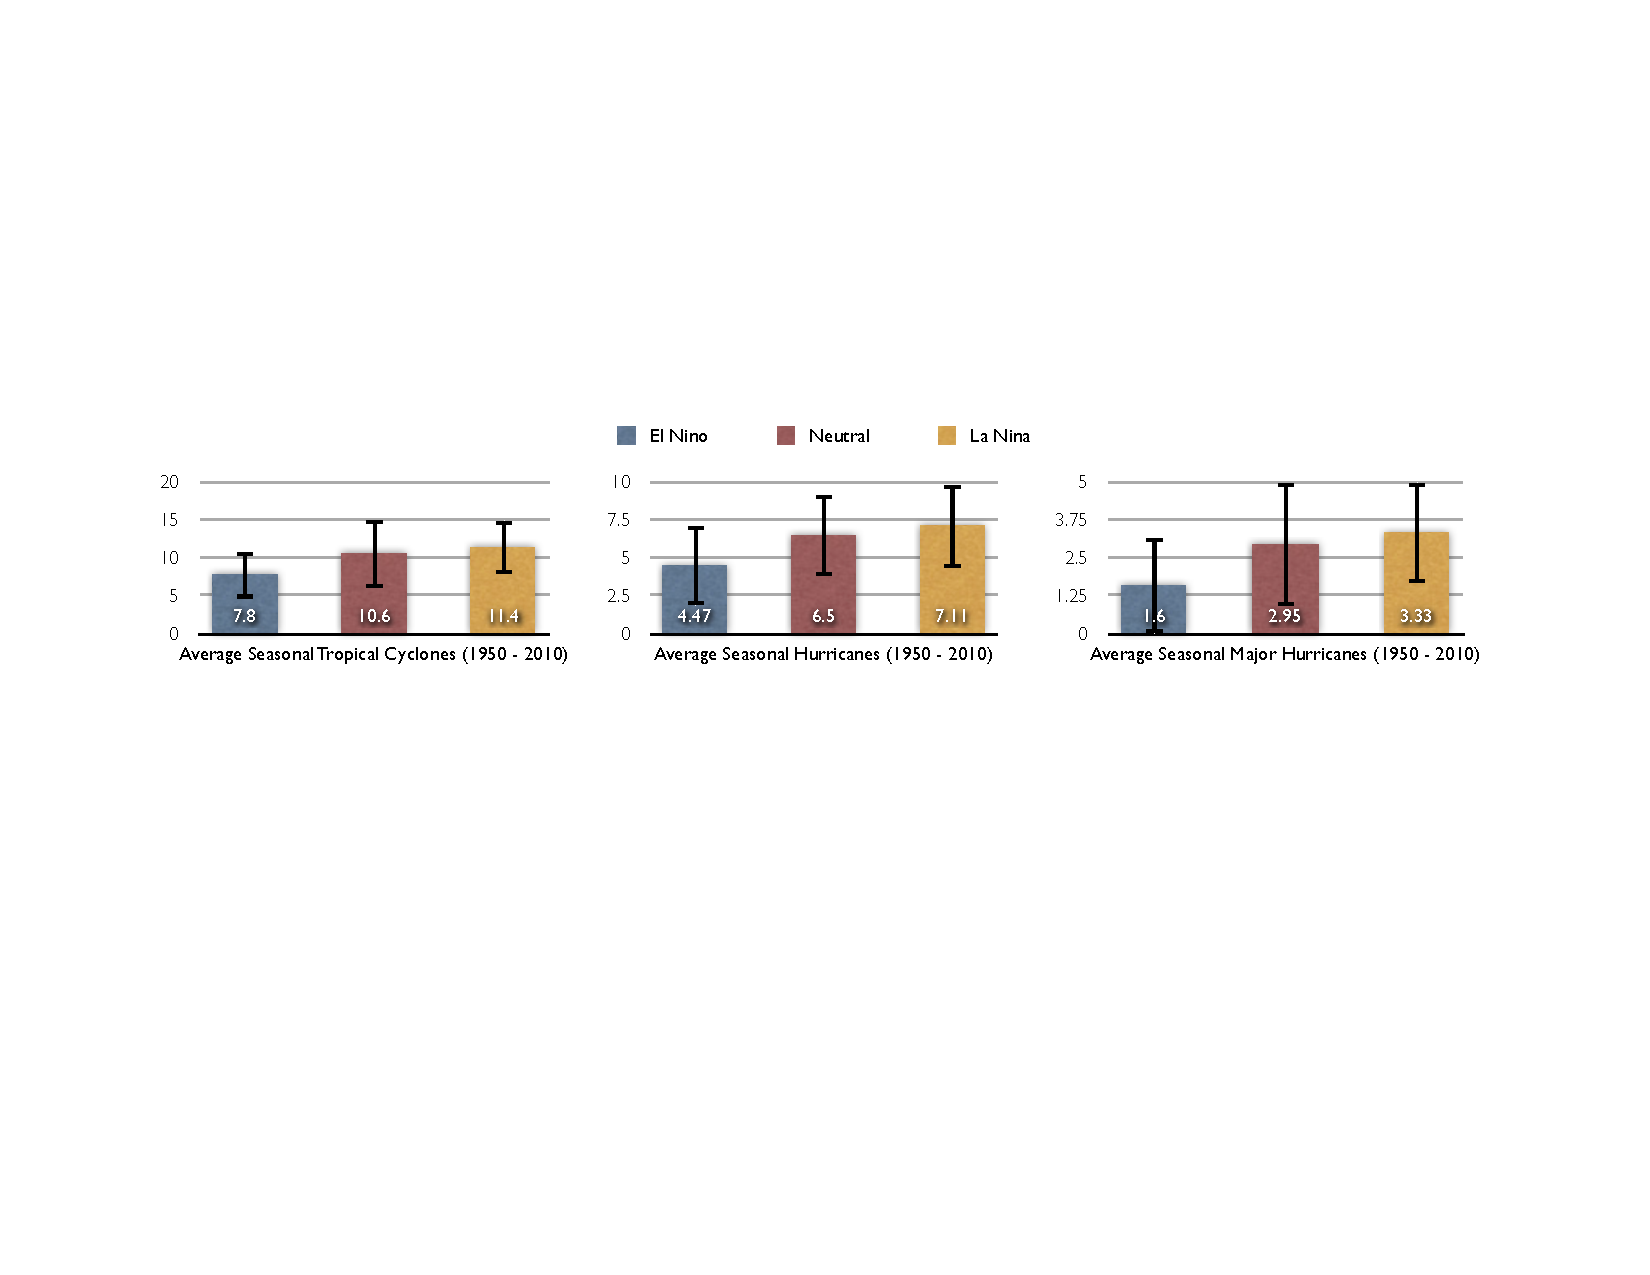
\includegraphics[width=5in]{figures/nino_nina_avg_diff.pdf}
	\caption{The $1950-2010$ seasonal mean Atlantic tropical cyclones (a), hurricanes (b), and major hurricane (c) counts for El-Ni\~no, neutral, and La Ni\~na years. Vertical bars denote standard deviation. The overlap between between bars across categories makes distinguishing between Atlantic TC activity based on the phase of ENSO uncertain.}
	\label{fig:enso_bars}
\end{figure}


%Given its long-range teleconnections, as well as ENSO being the most dominant feature of cyclic climate variability on subdecadal timescales, effectively abstracting and predicting Pacific Ocean warming anomalies has been a subject of active research. 


\section{Spatial ENSO Index (S-ENSO)}
We propose that the spatial distribution of Pacific Ocean warming might provide better predictive insights into ENSO-Atlantic TC activity relationship than warming anomalies alone. S-ENSO is a distance-based ENSO index that tracks the longitudinal location of highest SST anomaly in the tropical Pacific. We also track the mean Outgoing Longwave Radiation (OLR) of the identified region to monitor the atmospheric deep convection associated with such anomalies. The S-ENSO index is computed by first averaging the SST anomalies over the March-October period to accurately capture ENSO's evolution prior to and during the Atlantic hurricane season (August-October). We then search the tropical Pacific ($5^\circ$S-$30^\circ$N) for a region of similar size than traditional ENSO indices that has the highest mean SST anomaly over the March-October (see figure \ref{fig:s_enso_graphic}). Once such a region is identified, we compute the mean OLR over that region and use it as a single entry in the index. We repeat this procedure for each year from 1979 to 2010. Table \ref{ref:lin_corr} shows S-ENSO's linear correlation coefficients with various quantities that communicate August-October Atlantic TC activity: number of tropical cyclones, number of major hurricanes, potential dissipation index (PDI) \cite{emanuel2005a}, accumulated cyclone energy (ACE) \cite{Bell2000}, and net tropical cyclone energy (NTC) \cite{goldenberg2001}.

\begin{figure}[htbp]
	\centering
		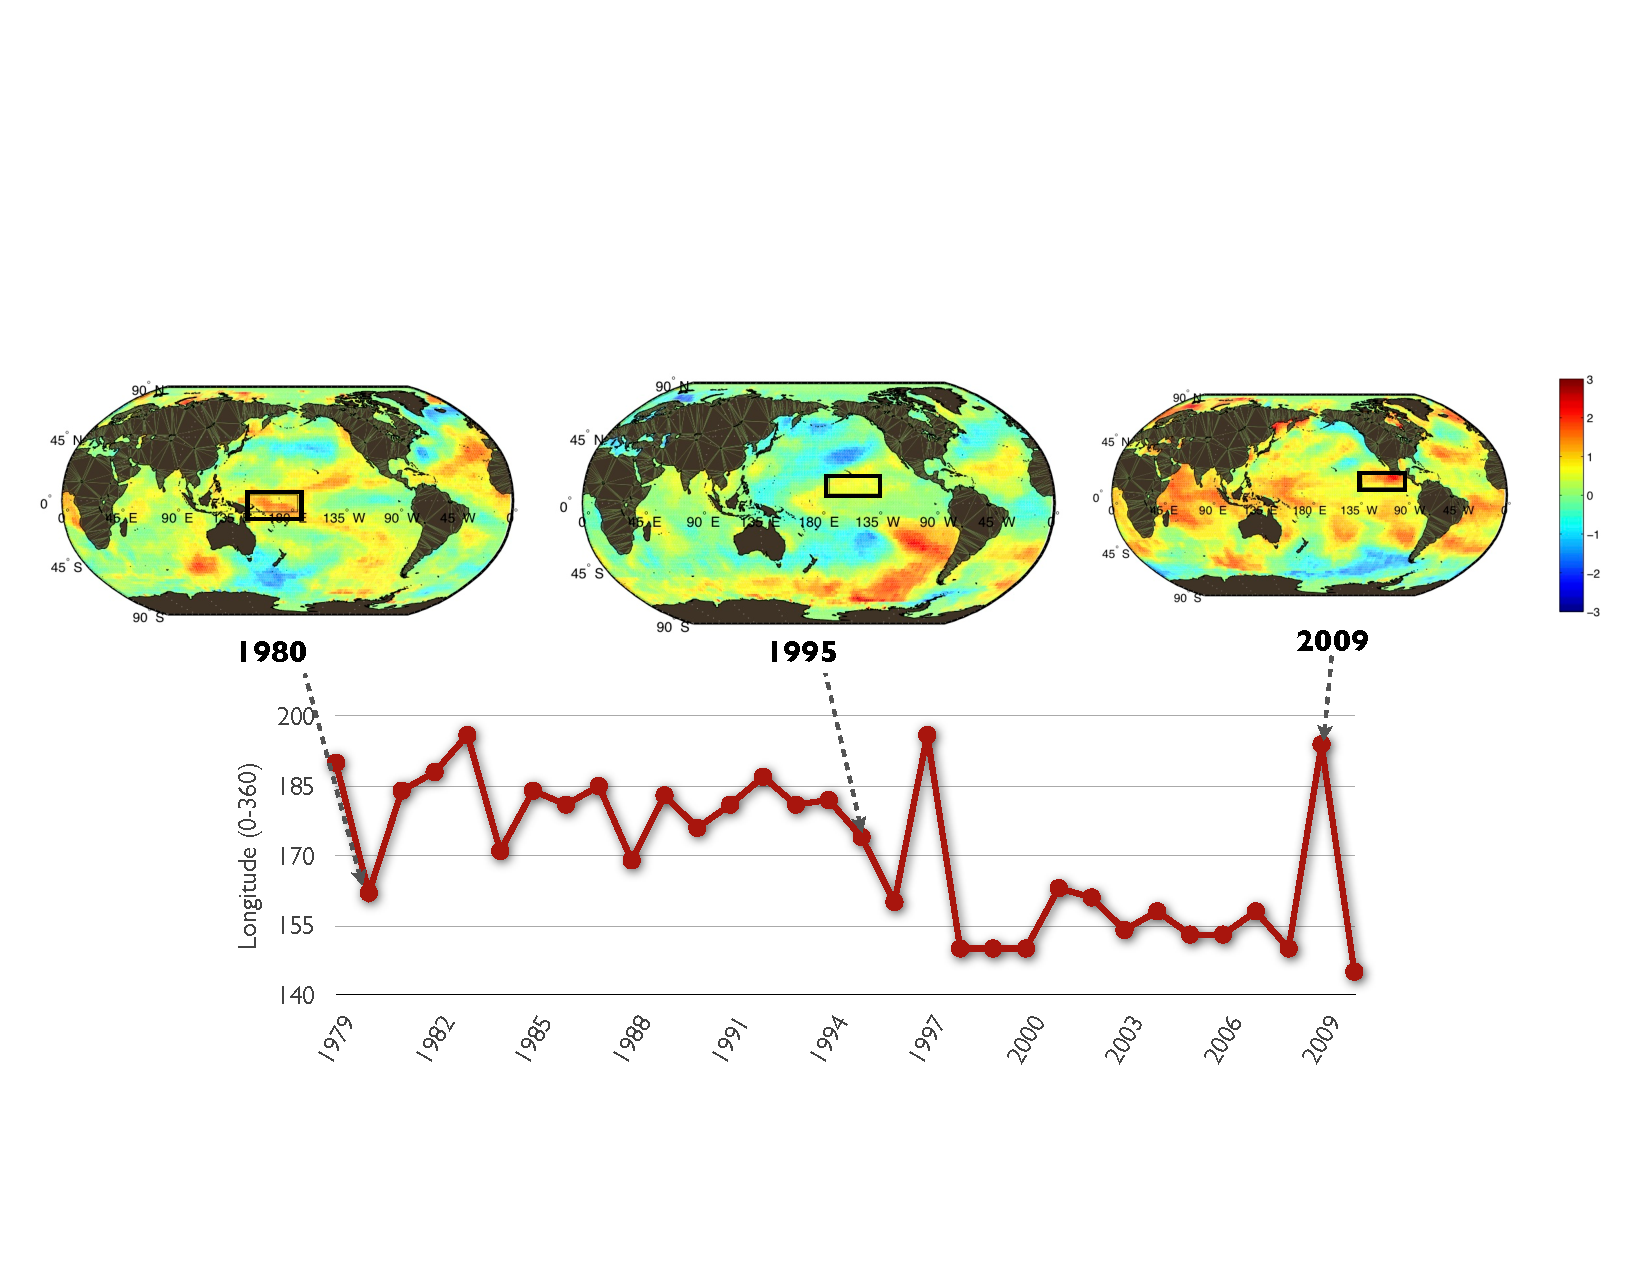
\includegraphics[width=5in]{figures/s_enso_graphic.pdf}
	\caption{A schematic demonstrating how the S-ENSO index is built. First, SST anomalies over March-October are computed resulting in maps similar to those above. Next, we search the tropical Pacific for the region with the highest mean SST warming anomaly over March-October. Finally, we record the longitude of that region. We repeat this procedure for all years from 1979-2010. }
	\label{fig:s_enso_graphic}
\end{figure}


\begin{figure}[htbp]
	\hspace{-1cm}
		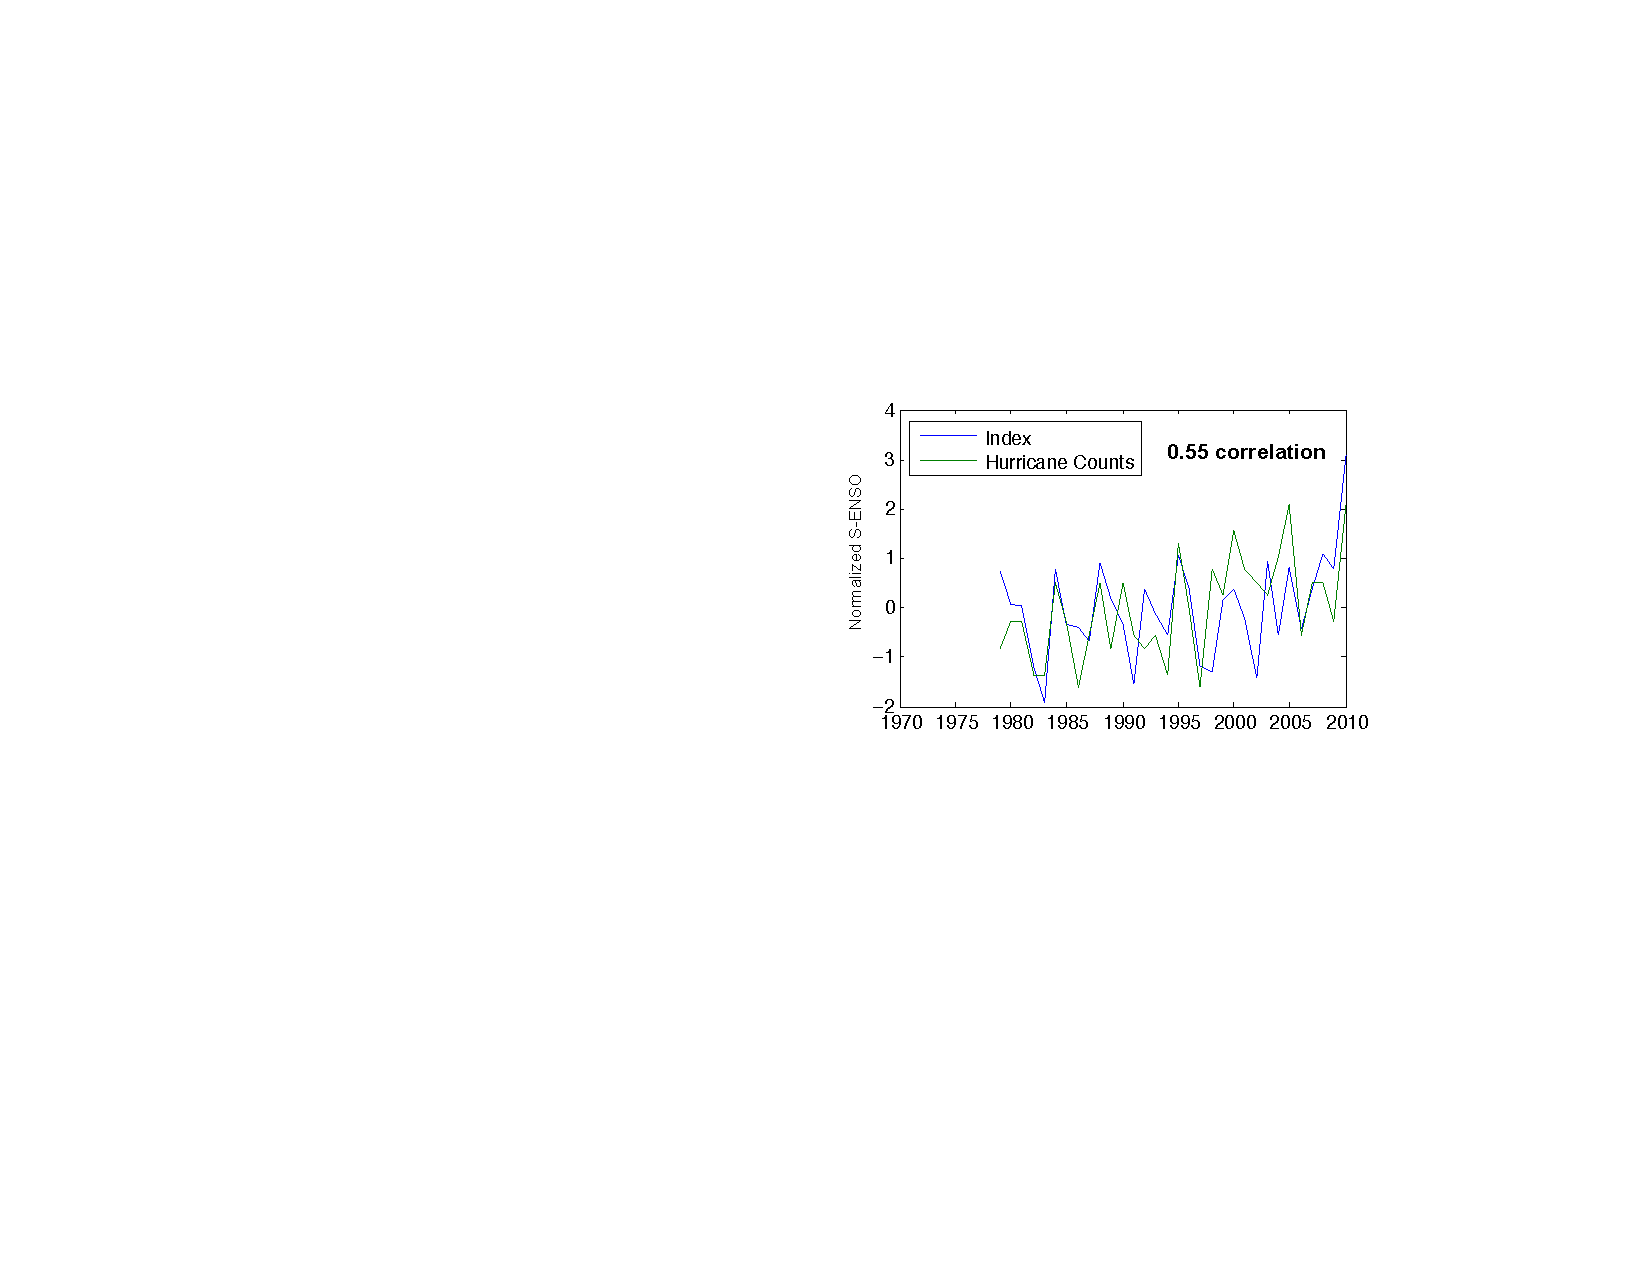
\includegraphics[width=5in]{figures/olr_corr.pdf}
	\caption{The time-series of S-ENSO along with annual August-October Atlantic TC counts.The mean OLR of the the warmest Pacific SST anomaly region and August-October Atlantic TC counts (0.55 linear correlation). There is a notable shift in the SST anomaly signal after 1997.}
	\label{fig:stbox_and_olr_ts}
\end{figure}


% distance between the location of maximum and minimum Pacific tropical warming anomalies instead of the absolute warming of a static region. The S-ENSO index consists of four factors: (i) the longitudinal distance between the warmest and coldest SST anomaly pool in the tropical Pacific, (ii) the mean Outgoing Longwave Radiation (OLR) of the warmest SST anomaly region in the tropical Pacific to monitor atmospheric deep convection, (iii) the mean surface pressure of the warmest SST anomaly region in the tropical Pacific, and (iv) the longitude of the minimal pressure region in the tropical Pacific to approximate Pacific tropical cyclone (typhoon) activity. The S-ENSO index is computed, by first averaging each variable over the March-October then building each of the four indices separately. Then we sum the normalized indices into a single S-ENSO index. For each year from 1979-2011, we search for the region of maximum and minimum warming anomaly in regions of size comparable to that of warming-based ENSO indices. The time series of the longitude of the PWP is then correlated with various quantities that communicate August-October Atlantic TC activity: number of tropical cyclones, number of major hurricanes, potential dissipation index (PDI) \cite{emanuel2005a}, accumulated cyclone energy (ACE) \cite{Bell2000}, and net tropical cyclone energy (NTC) \cite{goldenberg2001}.



% \begin{table}
% \hspace*{-1.5cm}
% \begin{tabular}{cc}
% \hline
% Acronym & Quantity\\
% \hline
% PWP-Lon & The longitude of the warmest SST pool in the northern near equatorial Pacific\\
% PWP-Pres & The mean presure of PWP\\
% PWP-OLR &  The mean OLR of PWP \\
% MinPres-Lon & The longitude of the region with the lowest mean central pressure\\
% PWP-PCP & The longitudinal distance between PWP and PCP \\
% Combo Index & A linear combination of xxxx \\
% \hline
% \end{tabular}
% \caption{A List of all quantities computed for this study with their corresponding acronyms.}
% \label{ref:acronyms}
% \end{table}

% Given that S-ENSO's performance depends on the month range over which the index is computed, we performed a month range sensitivity analysis to asses the robustness of our results with respect to month range selection. For every possible month range, we computed the S-ENSO, NINO1.2, NINO3, NINO4, and NINO3.4 indeces to correlated them with August-October Atlantic TC activity. Figure \ref{fig:tc_sensitivity} shows the month range sensitivity tests for NINO1.2, NINO3, NINO4, NINO3.4, and S-ENSO. Each cell color represents the the linear correlation coefficients between August-October TC Atlantic TC activity and the index computed over a given start and end month. S-ENSO performs significantly better than especially with increased lead times as NINO indices suffer from a ``predictability barrier" that make it difficult to use them to predict TC activity before June \cite{webster1992}.
% 
% \begin{figure}[htbp]
% 	\centering
% 		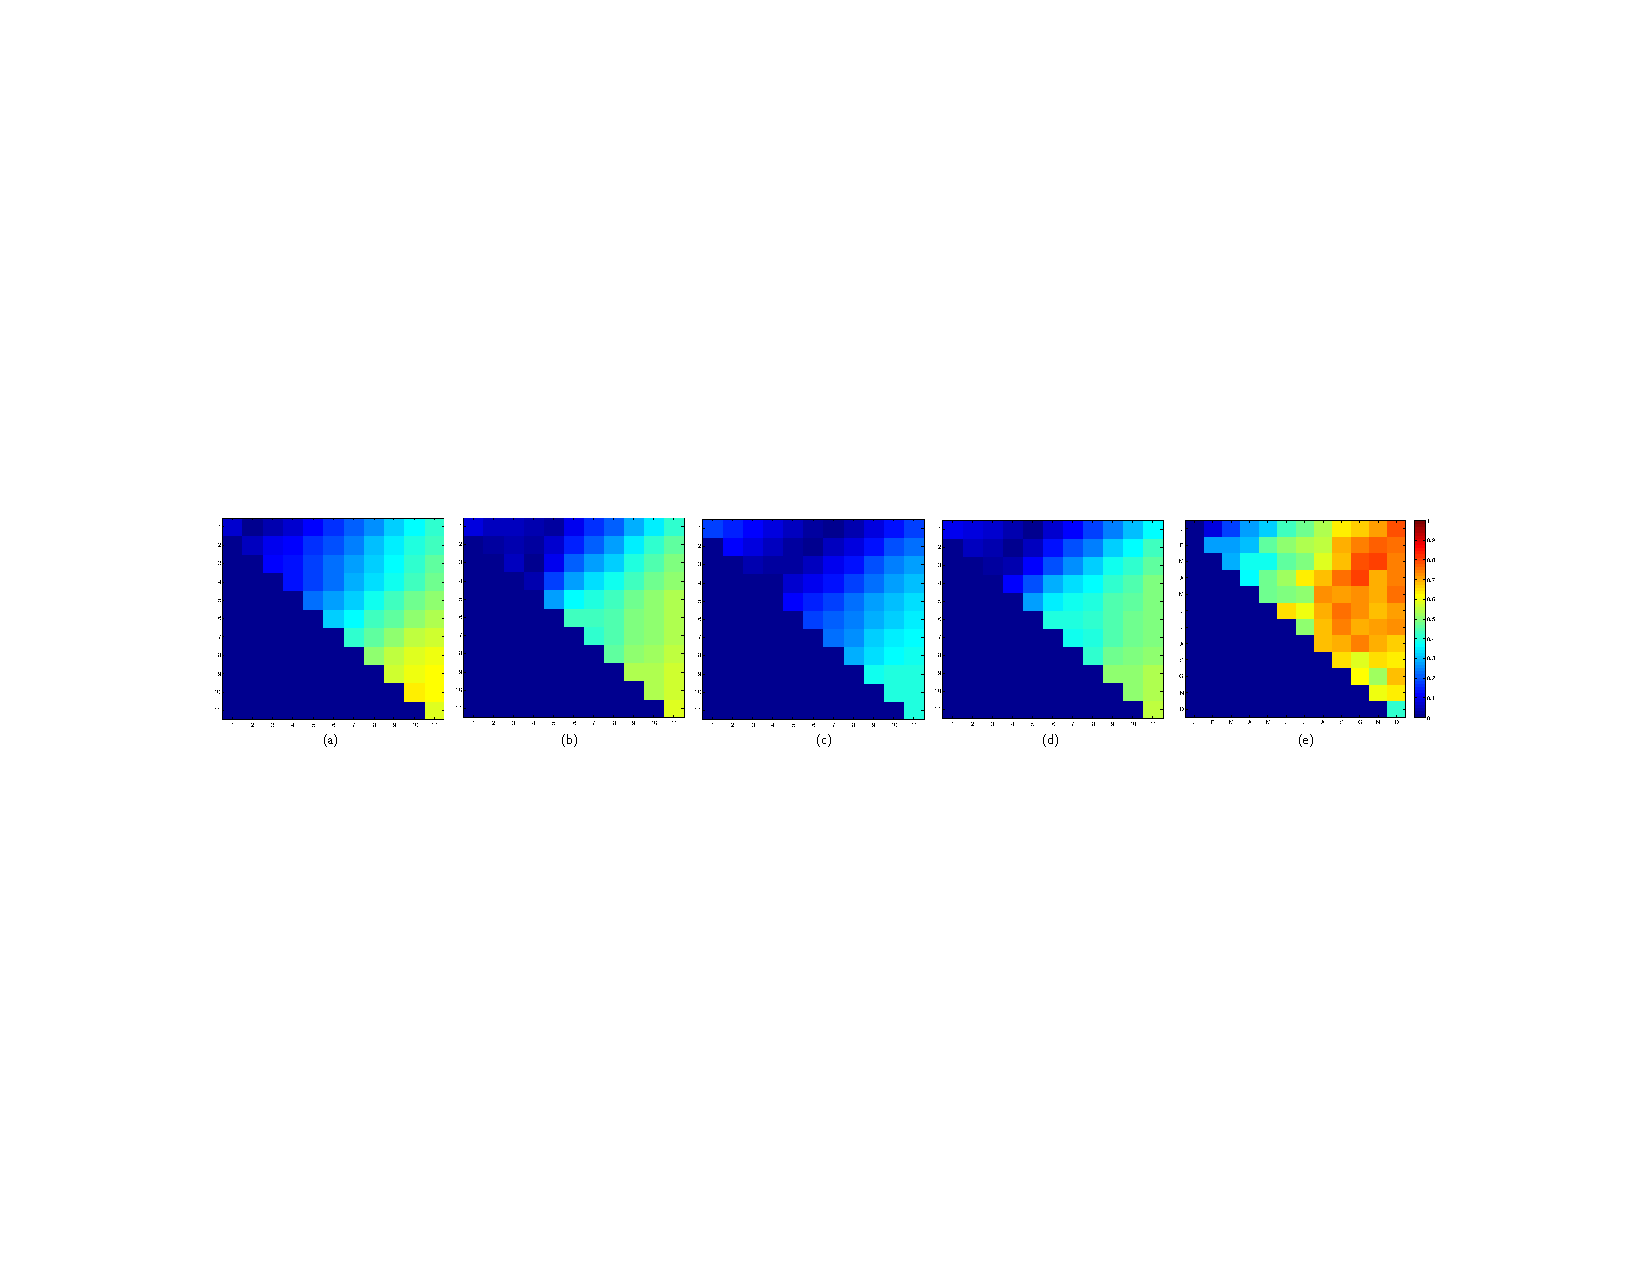
\includegraphics[width=5in]{figures/month_ranges_tcs.pdf}
% 	\caption{Month range sensitivity test for indices. (A) NINO1.2; (B) NINO3; (c) NINO4; (d) NINO3.4; (e) S-ENSO}
% 	\label{fig:tc_sensitivity}
% \end{figure}

\begin{table}
\begin{tabular}{cccccc}
\hline
&TCs & Major Hurricanes & NTC & PDI & ACE\\
\hline
%S-ENSO  & \textbf{0.81} & \textbf{0.81} & \textbf{0.77} & \textbf{0.71} & \textbf{0.75}\\
%PWP-Pres & 0.61 & 0.65 & 0.57 & 0.56 & 0.58\\
%PWP-OLR & 0.55 & 0.57 & 0.50 & 0.46 & 0.48\\
%MinPres-Lon & 0.15 & 0.12 & 0.19 & 0.17 & 0.20\\
%PWP-PCP  & 0.67 & 0.66 & 0.64 & 0.6 & 0.58\\
%maxSSTALon & \textbf{-0.64} & -0.5 & \textbf{-0.55} & -0.44 & \textbf{-0.49}\\
S-ENSO & \textbf{0.55} & \textbf{0.57} & 0.50 & \textbf{0.46} & \textbf{0.48}\\
Nino1+2 & -0.42 & -0.42 & -0.40 & -0.3 & -0.35\\
Nino 3 & -0.44 & -0.5 & -0.44 & -0.39 & -0.40\\
Nino 4 & -0.24 & -0.41 & -0.23 & -0.2 & -0.2\\
Nino 3.4 & -0.42 & -0.53 & -0.42 & -0.38 & -0.40\\
%Modoki Box A & -0.28 & -0 & -0.26 & -0.24 & -0.3\\
%Modoki Box B & -0.41 & -0.40 & -0.4 & -0 & -0.33\\
%Modoki Box C & 0.55 & 0.57 & 0.57 & 0.57 & 0.59\\
%Modoki EMI & -0.062 & -0.21 & -0.088 & -0.11 & -0.12\\
\hline
\end{tabular}
\caption{Linear correlation coefficients between the March-October S-ENSO and August-October Atlantic TC activity. The highest score for each category is highlighted in \textbf{bold}}
\label{ref:lin_corr}
\end{table}

% \subsection{Lead times}
% To test the robustness of our indices, we also increased computed the correlation between our indices and Atlantic TC activity with increasing lead times. Tables \ref{ref:lead_tc} and  \ref{ref:lead_hurr} show the correlations as a function of lead time for ASO TC and major hurricane counts respectively. The Combo Index has limited long range prediction as it doesn't have much skill until July for both hurricanes and TCs. Our SST-based indices (PWP-lon and PWP-PCP) have better long-range predictability. Our improvement over major NINO indices is significant with increased lead time (up to an order of magnitude better in some cases). This improvement is because traditional ENSO indices suffer from a ``predictability barrier" that make it difficult to use them to predict TC activity before June \cite{webster1992}. However, it is important to note that one static region in the Pacific (Modoki Box C) has good long-range correlations to both TCs and major hurricanes. However, that region alone isn't known to be used to TC or hurricane prediction. Another interesting observation, is the high correlation with both TCs and major hurricanes for the Jan-Dec month range for the Combo Index.
% 
% \begin{table}
% 	\hspace*{-3.5cm}
% \begin{tabular}{ccccccccccccc}
% \hline
% & Jan & Feb & Mar & Apr & May & Jun & Jul & Aug & Sep & Oct & Nov & Dec\\
% \hline
% Combo Index & -0.027 & 0.038 & 0.11 & 0.22 & 0.2 & 0.40 & 0.5 & \textbf{0.62} & \textbf{0.71} & \textbf{0.68} & \textbf{0.70} & \textbf{0.68}\\
% PWP-Pres &0.068 & 0.10 & 0.042 & 0.075 & 0.19 & 0.3 & 0.38 & 0.48 & 0.52 & 0.52 & 0.54 & 0.58\\
% PWP-OLR   & -0.35 & -0.21 & -0.13 & 0.03 & 0.054 & 0.2 & 0.21 & 0.4 & 0.48 & 0.50 & 0.51 & 0.57\\
% MinPres-Lon & -0.21 & -0.17 & -0.068 & -0.0013 & -0.37 & -0.18 & -0.095 & 0.025 & 0.094 & -0.14 & -0.13 & -0.25\\
% PWP-PCP  & \textbf{0.44} & 0.35 & 0.35 & 0.36 & 0.43 & 0.53 & 0.53 & 0.60 & 0.63 & 0.7 & 0.68 & 0.6\\
% PWP-lon & -0.3 & -0.36 & -0.38 & -0.37 & -0.39 & -0.4 & -0.53 & -0.53 & -0.55 & -0.56 & -0.59 & -0.56\\
% Nino1+2  & 0.053 & -0.0094 & -0.067 & -0.13 & -0.19 & -0.23 & -0.27 & -0.30 & -0.34 & -0.37 & -0.40 & -0.42\\
% Nino 3 & -0.011 & -0.036 & -0.044 & -0.077 & -0.15 & -0.22 & -0.28 & -0.33 & -0.39 & -0.44 & -0.48 & -0.51\\
% Nino 4 & -0.0090 & -0.036 & -0.056 & -0.076 & -0.11 & -0.15 & -0.19 & -0.24 & -0.28 & -0.33 & -0.37 & -0.40\\
% Nino 3.4  -0.026 & -0.061 & -0.074 & -0.11 & -0.16 & -0.23 & -0.29 & -0.34 & -0.40 & -0.45 & -0.49 & -0.53\\
% Modoki Box A  & -0.03 & -0.070 & -0.087 & -0.11 & -0.15 & -0.19 & -0.24 & -0.29 & -0.32 & -0.36 & -0.39 & -0.42\\
% Modoki Box B & 0.02 & -0.026 & -0.063 & -0.10 & -0.2 & -0.21 & -0.25 & -0.28 & -0.3 & -0.35 & -0.38 & -0.40\\
% Modoki Box C & 0.42 & \textbf{0.47} & \textbf{0.52} & \textbf{0.52} & \textbf{0.54} & \textbf{0.56} & \textbf{0.59} & 0.60 & 0.59 & 0.58 & 0.57 & 0.57\\
% Modoki EMI & -0.14 & -0.16 & -0.16 & -0.16 & -0.16 & -0.16 & -0.17 & -0.19 & -0.20 & -0.21 & -0.23 & -0.24\\
% \hline
% \end{tabular}
% \caption{Linear correlation scores between various indices computed over decreasing lead times and August-October Atlantic TC season counts. Each column header signifies the end month of the The highest score for each category is highlighted in \textbf{bold}}
% \label{ref:lead_tc}
% \end{table}
% 
% 
% 
% \begin{table}
% 	\hspace*{-3.5cm}
% \begin{tabular}{ccccccccccccc}
% \hline
% & Jan & Feb & Mar & Apr & May & Jun & Jul & Aug & Sep & Oct & Nov & Dec\\
% \hline
% Combo Index  & -0.12 & 0.020 & 0.074 & 0.19 & 0.29 & 0.40 & 0.45 & 0.57 & 0.58 & \textbf{0.67} & \textbf{0.72} & \textbf{0.76}\\
% PWP-Pres & 0.18 & 0.026 & 0.07 & 0 & 0.23 & 0.29 & 0.32 & 0.3 & 0.37 & 0.39 & 0.48 & 0.56\\
% PWP-OLR & -0.50 & -0.29 & -0.20 & -0.041 & 0.0039 & 0.13 & 0.17 & 0.28 & 0.35 & 0.4 & 0.42 & 0.50\\
% MinPres-Lon & -0.26 & 0.0025 & 0.015 & -0.025 & -0.11 & -0.11 & 0.0023 & 0.12 & 0.075 & 0.053 & 0.025 & -0.04\\
% PWP-PCP & \textbf{0.33} & 0.30 & 0.25 & 0.31 & \textbf{0.46} & \textbf{0.50} & 0.52 & 0.60 & 0.61 & 0.68 & 0.72 & 0.71\\
% PWP-lon  & -0.21 & -0.28 & -0.30 & -0.33 & -0.46 & -0.48 & \textbf{-0.62} & \textbf{-0.62 }& \textbf{-0.64} & -0.64 & -0.70 & -0.67\\
% Nino1+2 & 0.076 & 0.015 & -0.035 & -0.067 & -0.12 & -0.16 & -0.21 & -0.27 & -0.31 & -0.36 & -0.41 & -0.44\\
% Nino 3 & 0.084 & 0.061 & 0.06 & 0.041 & -0.023 & -0.096 & -0.16 & -0.22 & -0.29 & -0.36 & -0.42 & -0.47\\
% Nino 4 & 0.18 & 0.15 & 0.12 & 0.093 & 0.060 & 0.028 & -0.002 & -0.039 & -0.086 & -0.14 & -0.18 & -0.23\\
% Nino 3.4 & 0.10 & 0.082 & 0.067 & 0.04 & -0.0099 & -0.068 & -0.12 & -0.18 & -0.25 & -0.3 & -0.37 & -0.43\\
% Modoki Box A & 0.14 & 0.10 & 0.078 & 0.049 & 0.0057 & -0.03 & -0.071 & -0.12 & -0.15 & -0.19 & -0.23 & -0.26\\
% Modoki Box B & 0.016 & -0.018 & -0.04 & -0.051 & -0.10 & -0.17 & -0.22 & -0.26 & -0.31 & -0.36 & -0.41 & -0.44\\
% Modoki Box C & 0.29 & \textbf{0.34} & \textbf{0.39} & \textbf{0.41} & 0.44 & \textbf{0.5} & 0.51 & 0.55 & 0.55 & 0.54 & 0.54 & 0.54\\
% Modoki EMI & 0.081 & 0.044 & 0.020 & -0.0097 & -0.02 & -0.018 & -0.023 & -0.039 & -0.034 & -0.038 & -0.045 & -0.053\\
% \hline
% \end{tabular}
% \caption{Linear correlation scores between various indices computed over decreasing lead times and August-October Atlantic major hurricane (CAT 4-5) season counts. Each column header signifies the end month of the The highest score for each category is highlighted in \textbf{bold}}
% \label{ref:lead_hurr}
% \end{table}
% 
% \subsection{Seasonal TC forecasting}
% To asses our index' ability to forecast seasonal TC activity. We built a linear regression model using a leave k-out cross validation ($k=1,2,4,8$) Tables \ref{ref:l1o_corr} - \ref{ref:l8o_corr} show the results. We can see that our Combo Index is very robust regardless of how many observations are held out during training. However, it is important to note that the Modoki EMI index has an original correlation of -0.062 (no cross-validation) and a LOO cross-validation correlation of -0.56. It seems that straight non-random cross-validation might not fully address the ``Faghmous Paradox''
% 
% \begin{table}
% \begin{tabular}{cccccc}
% \hline
% & TC & Major Hurricanes & PDI & NTC & ACE\\
% \hline
% Combo Index & 0.78 & 0.79 & 0.68 & 0.7 & 0.71\\
% PWP-Pres & 0.6 & 0.59 & 0.50 & 0.5 & 0.53\\
% PWP-OLR & 0.47 & 0.51 & 0.35 & 0.41 & 0.38\\
% MinPres-Lon & -0.32 & -0.50 & -0.27 & -0.22 & -0.19\\
% PWP-PCP & 0.62 & 0.61 & 0.50 & 0.59 & 0.51\\
% PWP-lon & 0.6 & 0.4 & 0.31 & 0.47 & 0.37\\
% Nino1+2 & 0.30 & 0.32 & 0.17 & 0.27 & 0.18\\
% Nino 3 & 0.35 & 0.4 & 0.3 & 0.35 & 0.29\\
% Nino 4 & 0.0022 & 0.27 & -0.099 & -0.022 & -0.035\\
% Nino 3.4 & 0.31 & 0.45 & 0.27 & 0.33 & 0.30\\
% Modoki Box A & 0.090 & 0.32 & 0.011 & 0.07 & 0.049\\
% Modoki Box B & 0.30 & 0.30 & 0.14 & 0.24 & 0.15\\
% Modoki Box C & 0.49 & 0.50 & 0.5 & 0.51 & 0.53\\
% Modoki EMI & -0.55 & -0.11 & -0.5 & -0.51 & -0.44\\
% \hline
% \end{tabular}
% \caption{Linear correlation between actual and predicted ASO Atlantic TC activity using \textbf{Leave One Out} cross-validation for each our indices and standard NINO indices.}
% \label{ref:l1o_corr}
% \end{table}
% 
% 
% \begin{table}
% \begin{tabular}{cccccc}
% \hline
% & TC & Major Hurricanes & PDI & NTC & ACE\\
% \hline
% Combo Index & 0.79 & 0.79 & 0.66 & 0.74 & 0.70\\
% PWP-Pres & 0.57 & 0.59 & 0.48 & 0.50 & 0.5\\
% PWP-OLR & 0.48 & 0.51 & 0.34 & 0.41 & 0.37\\
% MinPres-Lon & -0.37 & -0.55 & -0.35 & -0.30 & -0.3\\
% PWP-PCP & 0.65 & 0.61 & 0.46 & 0.57 & 0.49\\
% PWP-lon & 0.60 & 0.39 & 0.29 & 0.46 & 0.36\\
% Nino1+2 & 0.32 & 0.31 & 0.14 & 0.25 & 0\\
% Nino 3 & 0.35 & 0.4 & 0.25 & 0.32 & 0.27\\
% Nino 4 & -0.025 & 0.23 & -0.23 & -0.13 & -0.15\\
% Nino 3.4 & 0.31 & 0.44 & 0.22 & 0.29 & 0.26\\
% Modoki Box A & 0.077 & 0.29 & -0.090 & -0.018 & -0.043\\
% Modoki Box B & 0.32 & 0.29 & 0.12 & 0.22 & 0.14\\
% Modoki Box C & 0.51 & 0.50 & 0.49 & 0.5 & 0.51\\
% Modoki EMI & -0.50 & -0.15 & -0.52 & -0.5 & -0.48\\
% \hline
% \end{tabular}
% \caption{Linear correlation between actual and predicted ASO Atlantic TC activity using \textbf{Leave Two Out} cross-validation for each our indices and standard NINO indices.}
% \label{ref:l2o_corr}
% \end{table}
% 
% \begin{table}
% \begin{tabular}{cccccc}
% \hline
% &TC & Major Hurricanes & PDI & NTC & ACE\\
% \hline
% Combo Index & 0.8 & 0.79 & 0.63 & 0.71 & 0.67\\
% PWP-Pres & 0.55 & 0.59 & 0.44 & 0.47 & 0.47\\
% PWP-OLR & 0.46 & 0.51 & 0.29 & 0.38 & 0.32\\
% MinPres-Lon & -0.37 & -0.40 & -0.40 & -0.33 & -0.34\\
% PWP-PCP & 0.65 & 0.62 & 0.42 & 0.5 & 0.45\\
% PWP-lon & 0.58 & 0.38 & 0.25 & 0.43 & 0.31\\
% Nino1+2 & 0.27 & 0.28 & 0.12 & 0.22 & 0.14\\
% Nino 3 & 0.29 & 0.38 & 0.18 & 0.25 & 0.2\\
% Nino 4 & -0.11 & 0.15 & -0 & -0.26 & -0.29\\
% Nino 3.4 & 0.2 & 0.40 & 0.11 & 0.19 & 0.15\\
% Modoki Box A & -0.0038 & 0.2 & -0.23 & -0.14 & -0.18\\
% Modoki Box B & 0.27 & 0.26 & 0.081 & 0.17 & 0.098\\
% Modoki Box C & 0.48 & 0.48 & 0.44 & 0.46 & 0.46\\
% Modoki EMI & -0.56 & -0.23 & -0.6 & -0.60 & -0.56\\
% \hline
% \end{tabular}
% \caption{Linear correlation between actual and predicted ASO Atlantic TC activity using \textbf{Leave Four Out} cross-validation for each our indices and standard NINO indices.}
% \label{ref:l4o_corr}
% \end{table}
% 
% \begin{table}
% \begin{tabular}{cccccc}
% \hline
% & TC & Major Hurricanes & PDI & NTC & ACE\\
% \hline
% Combo Index & 0.77 & 0.78 & 0.65 & 0.72 & 0.67\\
% PWP-Pres & 0.49 & 0.53 & 0.42 & 0.44 & 0.43\\
% PWP-OLR & 0.35 & 0.44 & 0.25 & 0.32 & 0.25\\
% MinPres-Lon & -0.55 & -0.54 & -0.49 & -0.45 & -0.46\\
% PWP-PCP & 0.64 & 0.61 & 0.43 & 0.6 & 0.45\\
% PWP-lon & 0.55 & 0.35 & 0.2 & 0.4 & 0.25\\
% Nino1+2 & 0.12 & 0.15 & 0.0052 & 0.096 & 0.0055\\
% Nino 3 & 0.16 & 0.2 & 0.051 & 0.14 & 0.053\\
% Nino 4 & -0.25 & -0.00059 & -0.52 & -0.42 & -0.45\\
% Nino 3.4 & 0.13 & 0.27 & -0.046 & 0.073 & 0.0024\\
% Modoki Box A & -0.2 & 0.042 & -0.44 & -0.34 & -0.38\\
% Modoki Box B & 0.12 & 0.13 & -0.026 & 0.060 & -0.031\\
% Modoki Box C & 0.45 & 0.47 & 0.47 & 0.47 & 0.48\\
% Modoki EMI & -0.57 & -0.37 & -0.66 & -0.64 & -0.63\\
% \hline
% \end{tabular}
% \caption{Linear correlation between actual and predicted ASO Atlantic TC activity using \textbf{Leave Eight Out} cross-validation for each our indices and standard NINO indices.}
% \label{ref:l4o_corr}
% \end{table}


\section{S-ENSO's impact on large-scale conditions over the Atlantic}
To propose possible physical pathways by which our index impact Atlantic TC activity, we compute the composites for factors known to influence Atlantic TC activity: potential intensity (PI), saturation deficit between the mid- and lower-troposphere and vertical wind shear between 850 and 200 hPa. (also not shown we have composites for SST, central pressure, geopotential height and precipitable water). Each composite was for the August-October period - the peak hurricane season. To compare how well our index resolves the large-scale conditions that are critical to seasonal TC activity we compare our index' composites to those of the seasonal TC count composites (baseline) and those of the most common warming-based ENSO index: NINO3.4. The idea is that if our index is better able to distinguish between the large-scale conditions for active and inactive hurricane seasons its composites should closely resemble those of the baseline (i.e. active minus inactive hurricane years). Furthermore, Recent hurricane downscaling studies \cite{knutson2007simulation, emanuel2010comparison} as well as genesis indices \cite{menkes2012comparison} have shown that the large scale environment over the Atlantic might play a dominant role in modulating Atlantic TC activity than precursor disturbances, since these simulations do not model such disturbances yet are able to reproduce Atlantic TC climatology with significant accuracy.

%Figure \ref{fig:olr_comp} shows the composites for PI (top row), the difference in saturation deficit between 500 and 850 hPa (middle row), and vertical wind shear between 200 and 850 hPa (bottom) row. Each column shows the composites for hurricane counts (left), NINO3.4 (middle), and S-ENSO (right). $95\%$ significance intervals are shaded.

%Figure \ref{fig:pi_comp_vs_olr} shows the PI composite. S-ENSO is able to reproduce nearly identical conditions to those of the TC count composite. In figure \ref{fig:sat_def_comp} a linear combination of the S-ENSO and OLR is also able to reproduce the large-scale saturation deficit in the lower and middle troposphere. These results show that monitoring the spatial warming patterns of the tropical pacific can significantly increase our ability to resolve the large-scale conditions over the Atlantic during the hurricane season. 

Previous work investigating the ENSO-Atlantic TC teleconnection proposed that enhanced convection as a result of anomalous Pacific Ocean warming during the El Niño phase is associated with strong westerly upper tropospheric wind over the Caribbean basin and tropical Atlantic, resulting in low TC activity during ENSO's warm phase (El Ni\~{n}o) events and high TC activity during its cold phase (La Ni\~{n}a). Warm eastern Pacific SST and negative (drought) Sahelian rainfall anomalies are associated with suppressed Atlantic basin tropical cyclone activity through an equatorially confined near-zonal circulation with upper-level westerlies and lower-level easterlies that act to increase the climatological westerly vertical shear in the main development region \cite{goldenberg1996physical}. Other studies have suggested that ENSO impact Atlantic TC activity via tropospheric warming \cite{tang2004}, since warm free tropospheric temperatures that are spread eastward from the Pacific by equatorial wave dynamics (e.g. Kelvin waves) can inhibit TC activity by providing a too weak vertical temperature gradient for TC activity to occur. Analogous to reduced vertical temperature gradient, a reduced vertical gradient of saturation deficit suppresses vertical mixing and thus negatively affects TC activity.

However, it seems that by monitoring the deep convection associated with the region with the highest Pacific SST warming anomaly, we succeed to observe the strength and location of updrafts related to this convection and the resulting strength and location of the zonal Walker circulation, as well as its impact on the tropical Atlantic circulation, as described in e.g. \cite{liu2004remote}, who  suggest that the remote impact contributes to nearly half of the variance of the tropical Atlantic SST variability at interannual and decadal time scales. Updrafts over the eastern and central Pacific during El Ni\~no result in downdrafts and therefore reduced TC activity over the tropical Atlantic, whereas updrafts over the western Pacific during neutral and La Ni\~na years result in downdrafts over the eastern tropical Pacific and updrafts over the Atlantic, thus leading to increased TC activity.

\begin{figure}[htbp]

\hspace{-2.5cm}		
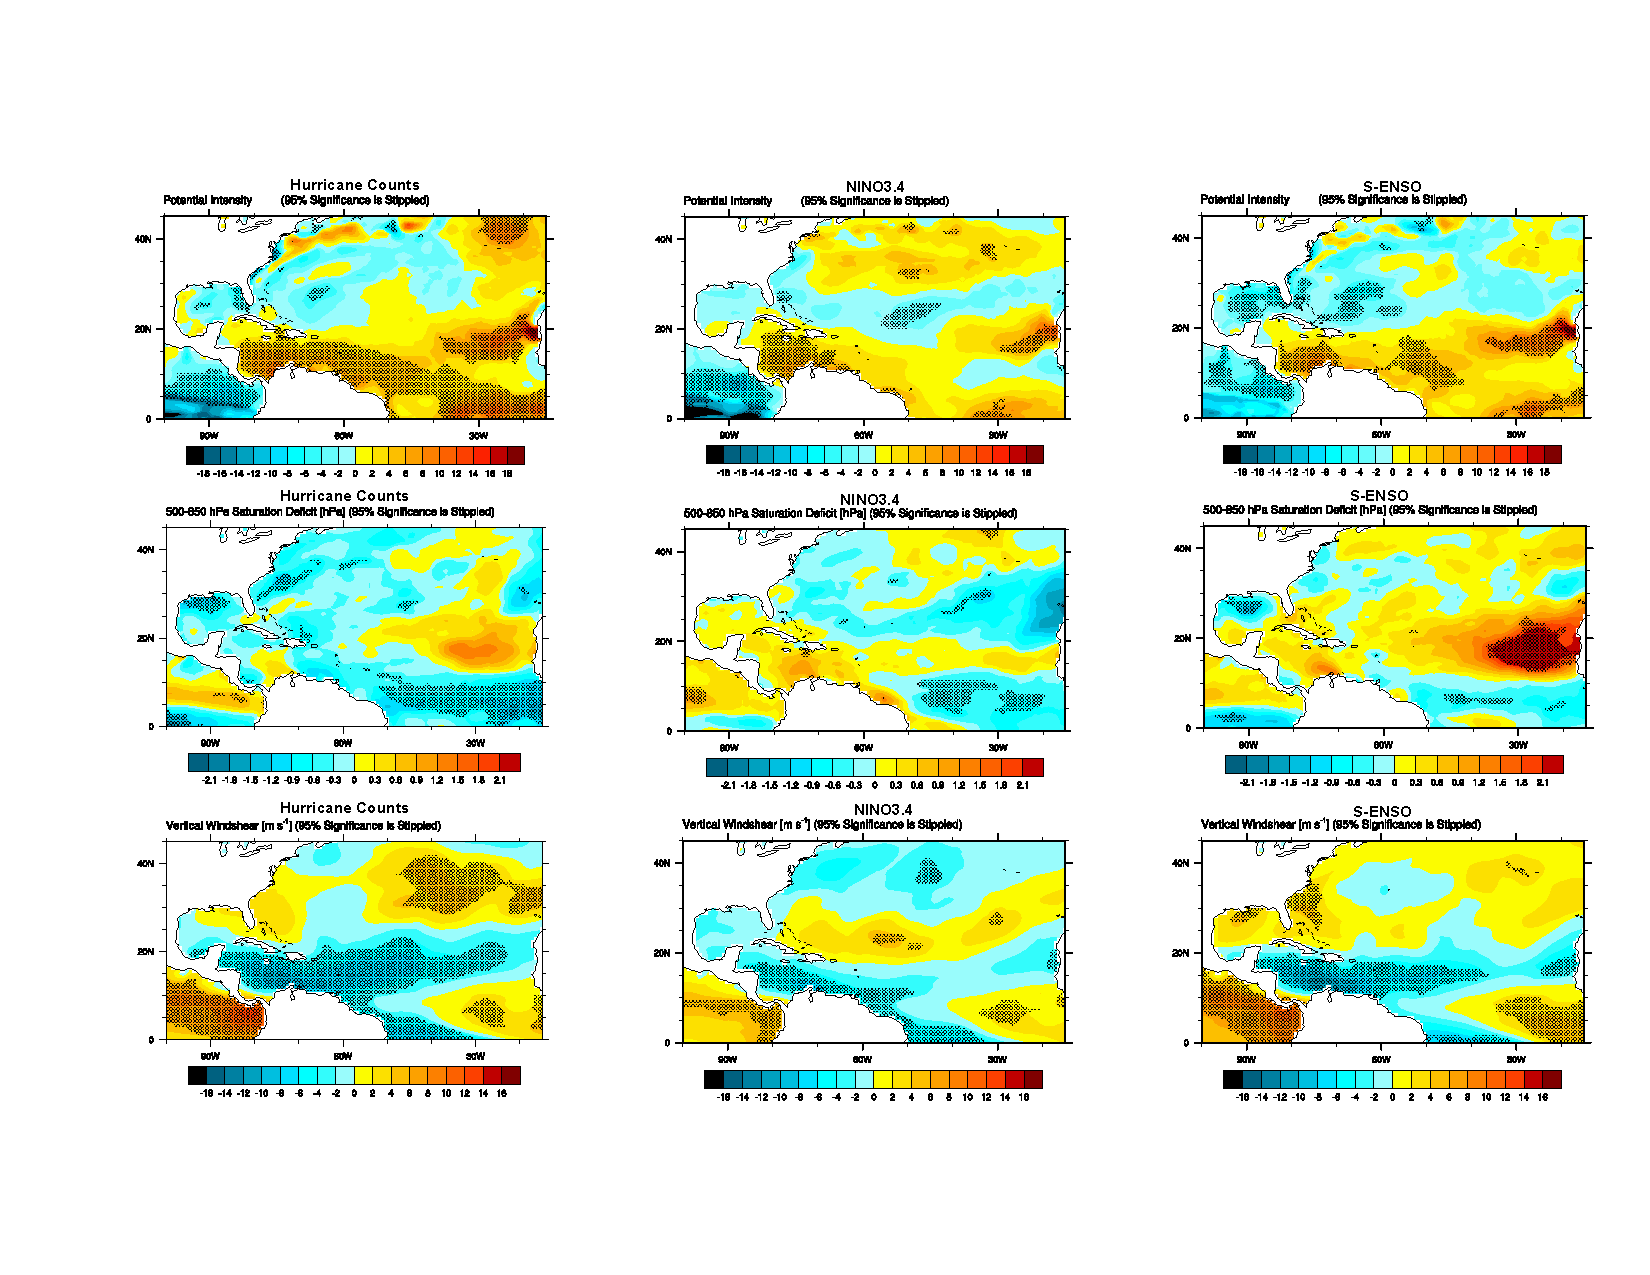
\includegraphics[width=7in]{figures/3_by_3_composites.pdf}
	\caption{composites for PI (top row), the difference in saturation deficit between 500 and 850 hPa (middle row), and vertical wind shear between 200 and 850 hPa (bottom) row. Each column shows the composites for hurricane counts (left), NINO3.4 (middle), and S-ENSO (right). $95\%$ significance intervals are shaded. Shaded area represents $95\%$ significance level. The hurricane count positive years (6) are: 1995, 2001, 2003, 2005, 2008, and 2010. The hurricane count negative years (8) are: 1982, 1983, 1986, 1987, 1992, 1993, 1994, 1997 and 2002. The NINO3.4 positive years (8) are: 1981, 1984, 1985, 1988, 1999, 2000, 2007, and 2008. The NINO3.4 negative years (6) are: 1982, 1987, 1991, 1992, 1997, 2002. S-ENSO positive years (6) are: 1989, 1995, 2003, 2005, 2008, 2010. S-ENSO negative years (6) are: 1982, 1983, 1991, 1997, 1998, 2002. For all three variables, S-ENSO reproduces the large scale environment over the Atlantic better than the traditional warming-based ENSO index NINO3.4}
	\label{fig:olr_comp}
\end{figure}


% \begin{figure}[htbp]
% 	\centering
% 		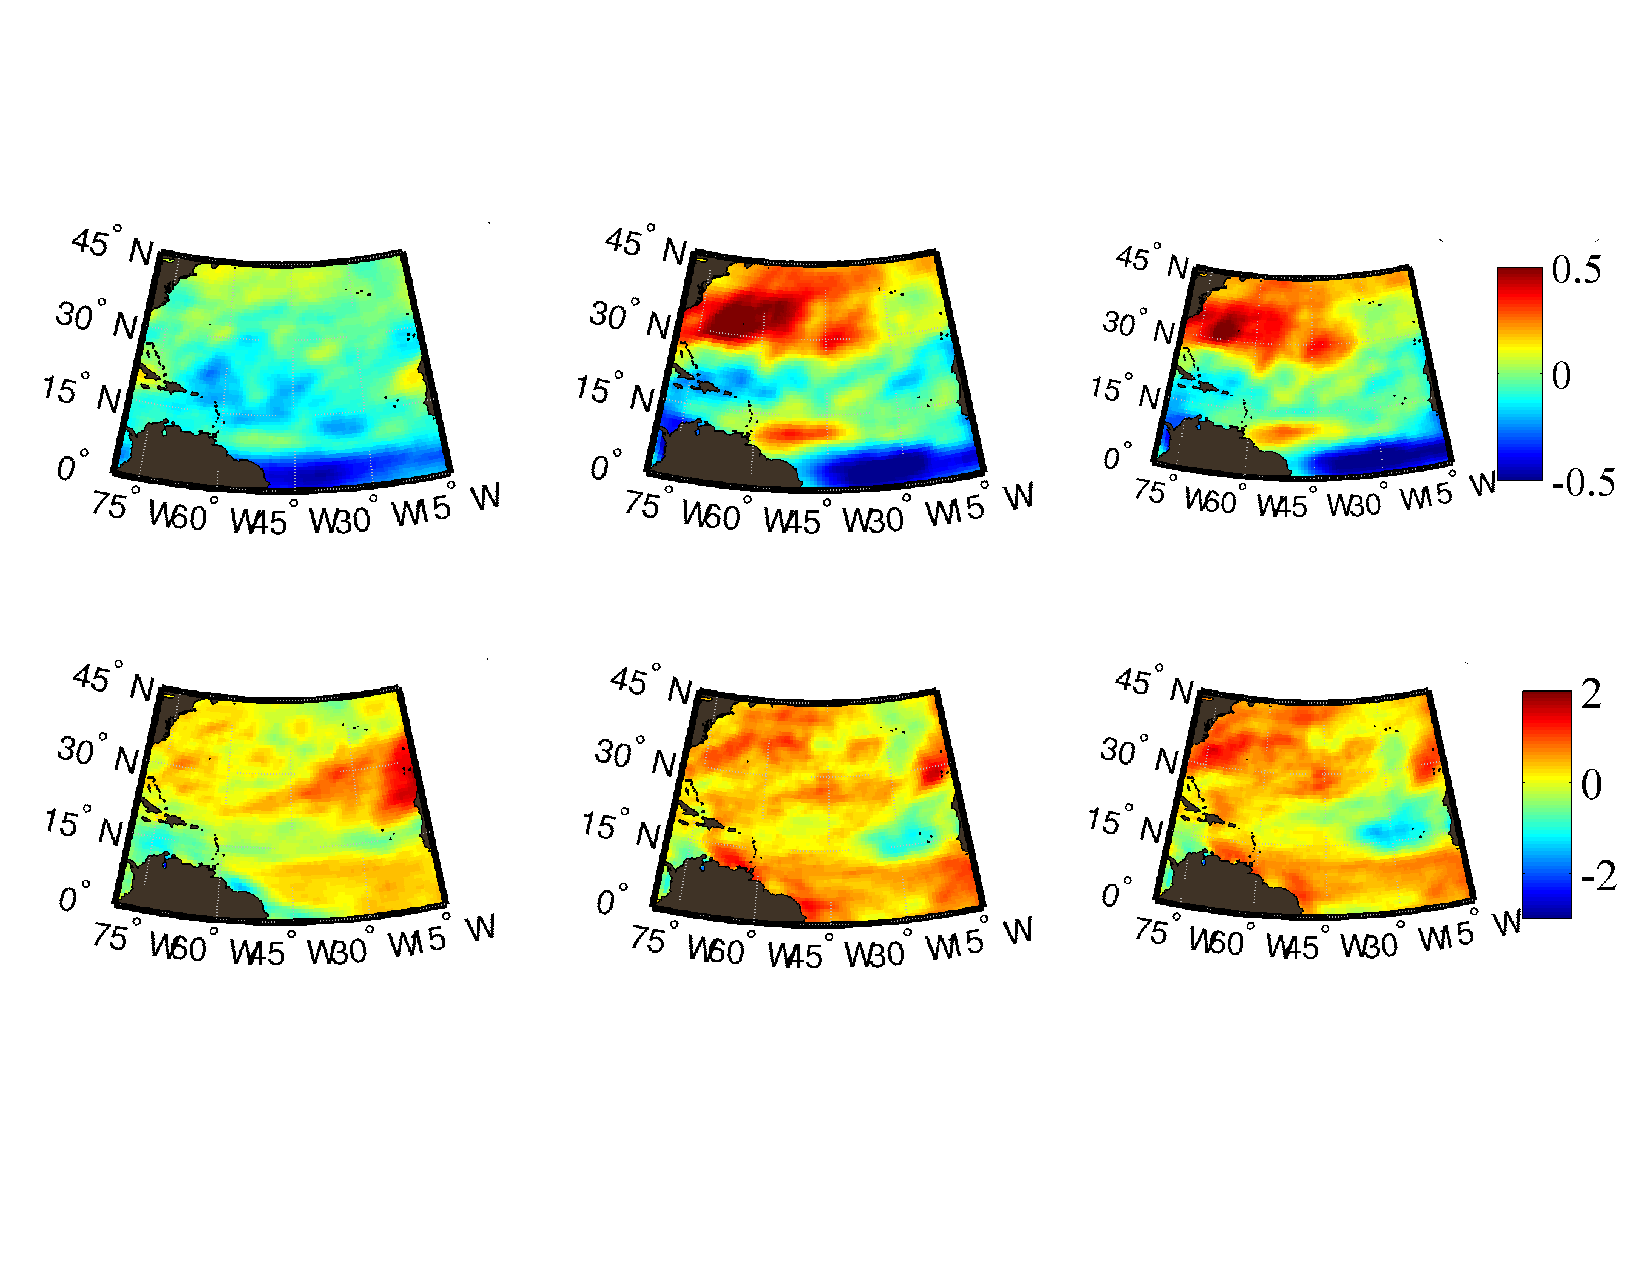
\includegraphics[width=5in]{figures/sat_def_comp.pdf}
% 	\caption{Saturation deficit composites at 500mb (top row) and 850 (bottom row). Left: NINO3.4 composite. Middle: the composite of a linear combination of the S-ENSO and OLR indices. Right: August-October Atlantic TC count composite. Our index is able to reproduce the saturation deficit the lower and middle troposphere over the Atlantic.}
% 	\label{fig:sat_def_comp} 
% \end{figure}

% \section{Appendix}
% We repeated the composite experiment presented in the text using the potential dissipation index as our the basis. Years that had a PDI value higher or lower than one standard deviation were used to composite PI, saturation deficit and vertical wind shear. 


\section{Acknowledgments}
We thank Prof. David Nolan for providing us with the MATLAB routines to compute potential intensity (PI) from reanalysis data.
\end{comment}
% Figures \ref{fig:pres_comp} - \ref{fig:figure37} show the composites (active years minutes inactive years) for NINO3.4 (top), Combo Index (middle) and ground truth (bottom).
% \subsubsection{Central Pressure}
% Tropical cyclones are low pressure systems, therefore seasons with high TC activity tend to have low pressure means as seen in Figure \ref{fig:pres_comp}. Our index is able to resolve much lower central pressure across the Atlantic Main Development Region (MDR) than the NINO3.4 index. It is not clear from this composite whether high TC activity is a cause or effect of large-scale low pressure.
% 
% 
% \subsubsection{Potential Intensity (PI)}
% Potential intensity is a variable computed by combining the column integrated air temperature and relative humidity. PI has been shown to provide the theoretical upper bound on storm intensity given air temperature and relative humidity \cite{emanuel1999}. PI has also been used as a proxy of how conducive an environment is for tropical cyclogenesis \cite{emanuel2008}. As shown in Figure \ref{fig:pi_comp} (bottom), active TC seasons tend to have high PI values along the MDR especially right off the West African coast where African Easterly Waves (AEWs) exit the continental mass. Similar to central pressure, our index (Figure \ref{fig:pi_comp} middle panel) resolves similar spatial patterns for PI than the ground truth.


% \begin{figure}[ht]
% \begin{minipage}[b]{0.55\linewidth}
% 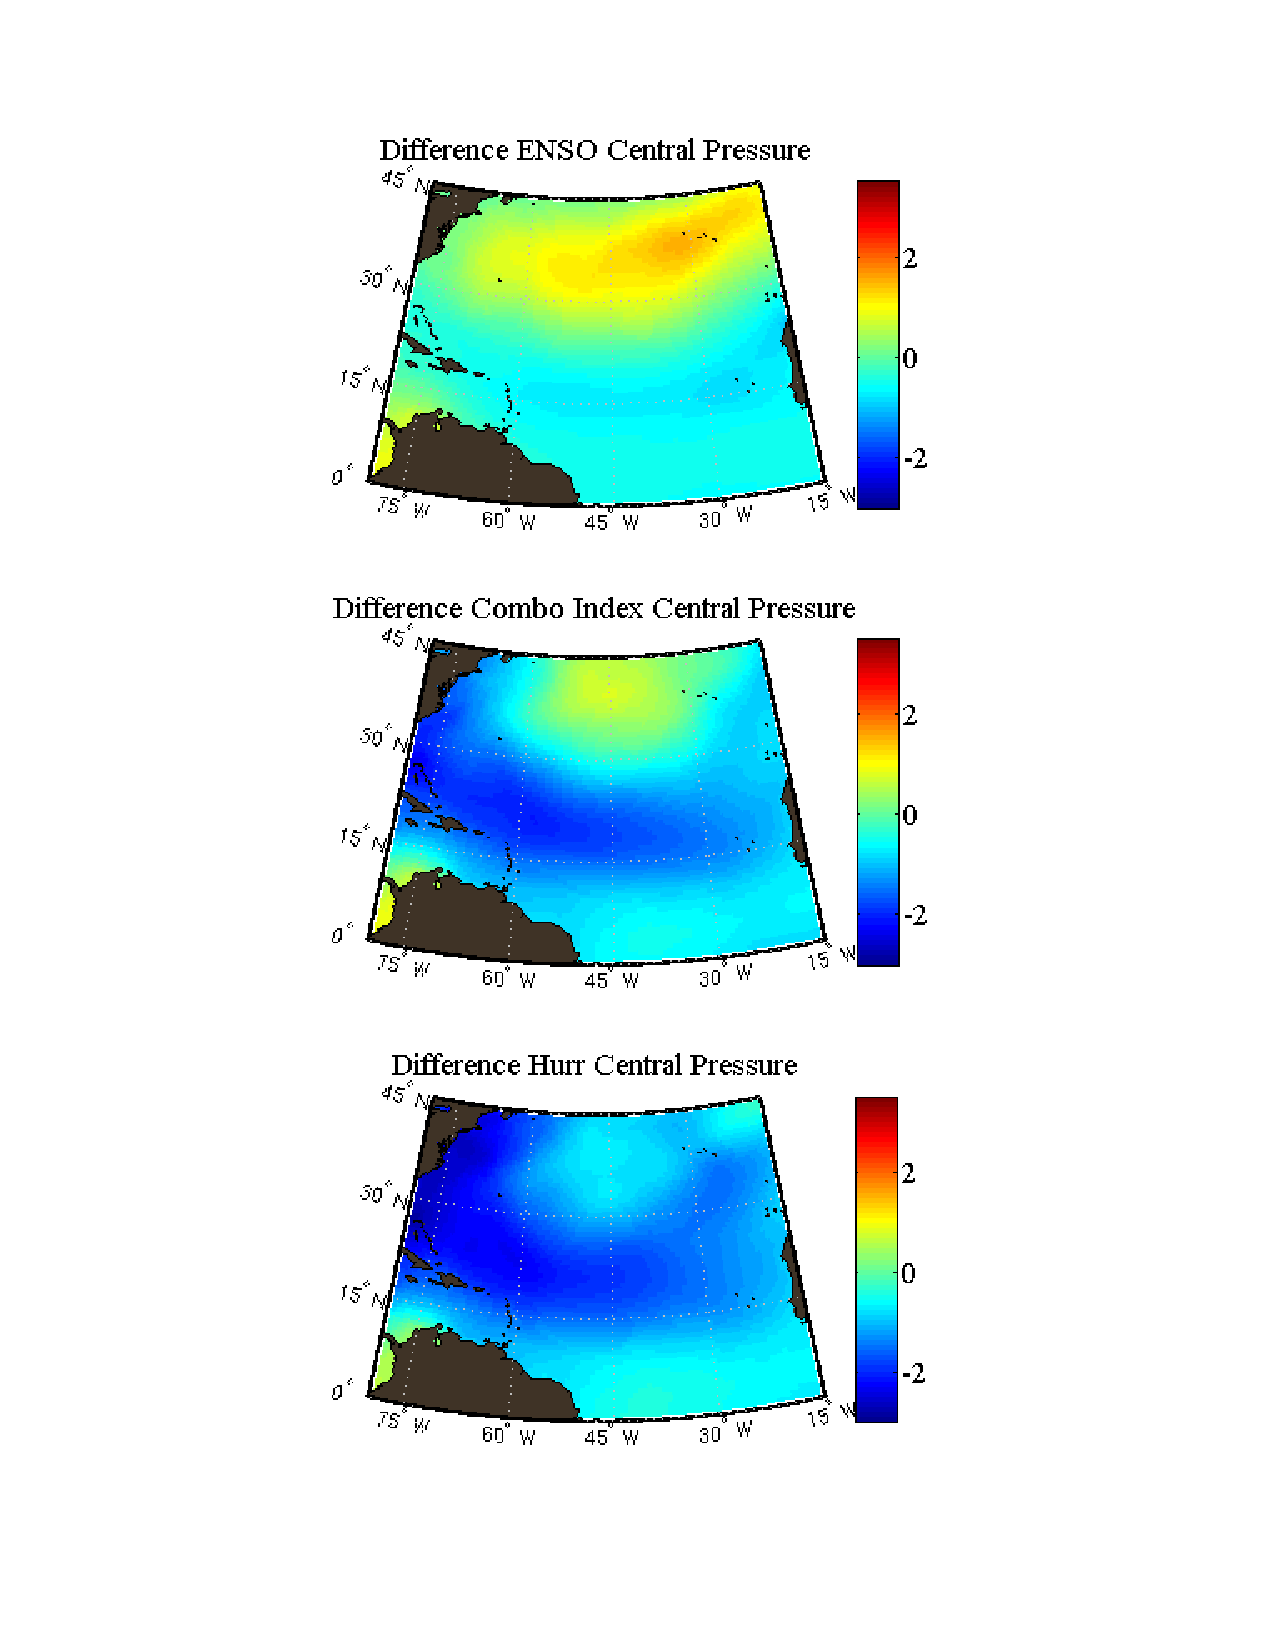
\includegraphics[width=\textwidth]{figures/comboIndex/composites/compareMDRCompositesCentralPressure.pdf}
% \caption{Central pressure composites for NINO3.4 (top), Combo Index (Middle), and Ground Truth (Bottom). Active TC seasons tend to have low pressure.}
% \label{fig:pres_comp}
% \end{minipage}
% \hspace{0.3cm}
% \begin{minipage}[b]{0.55\linewidth}
% 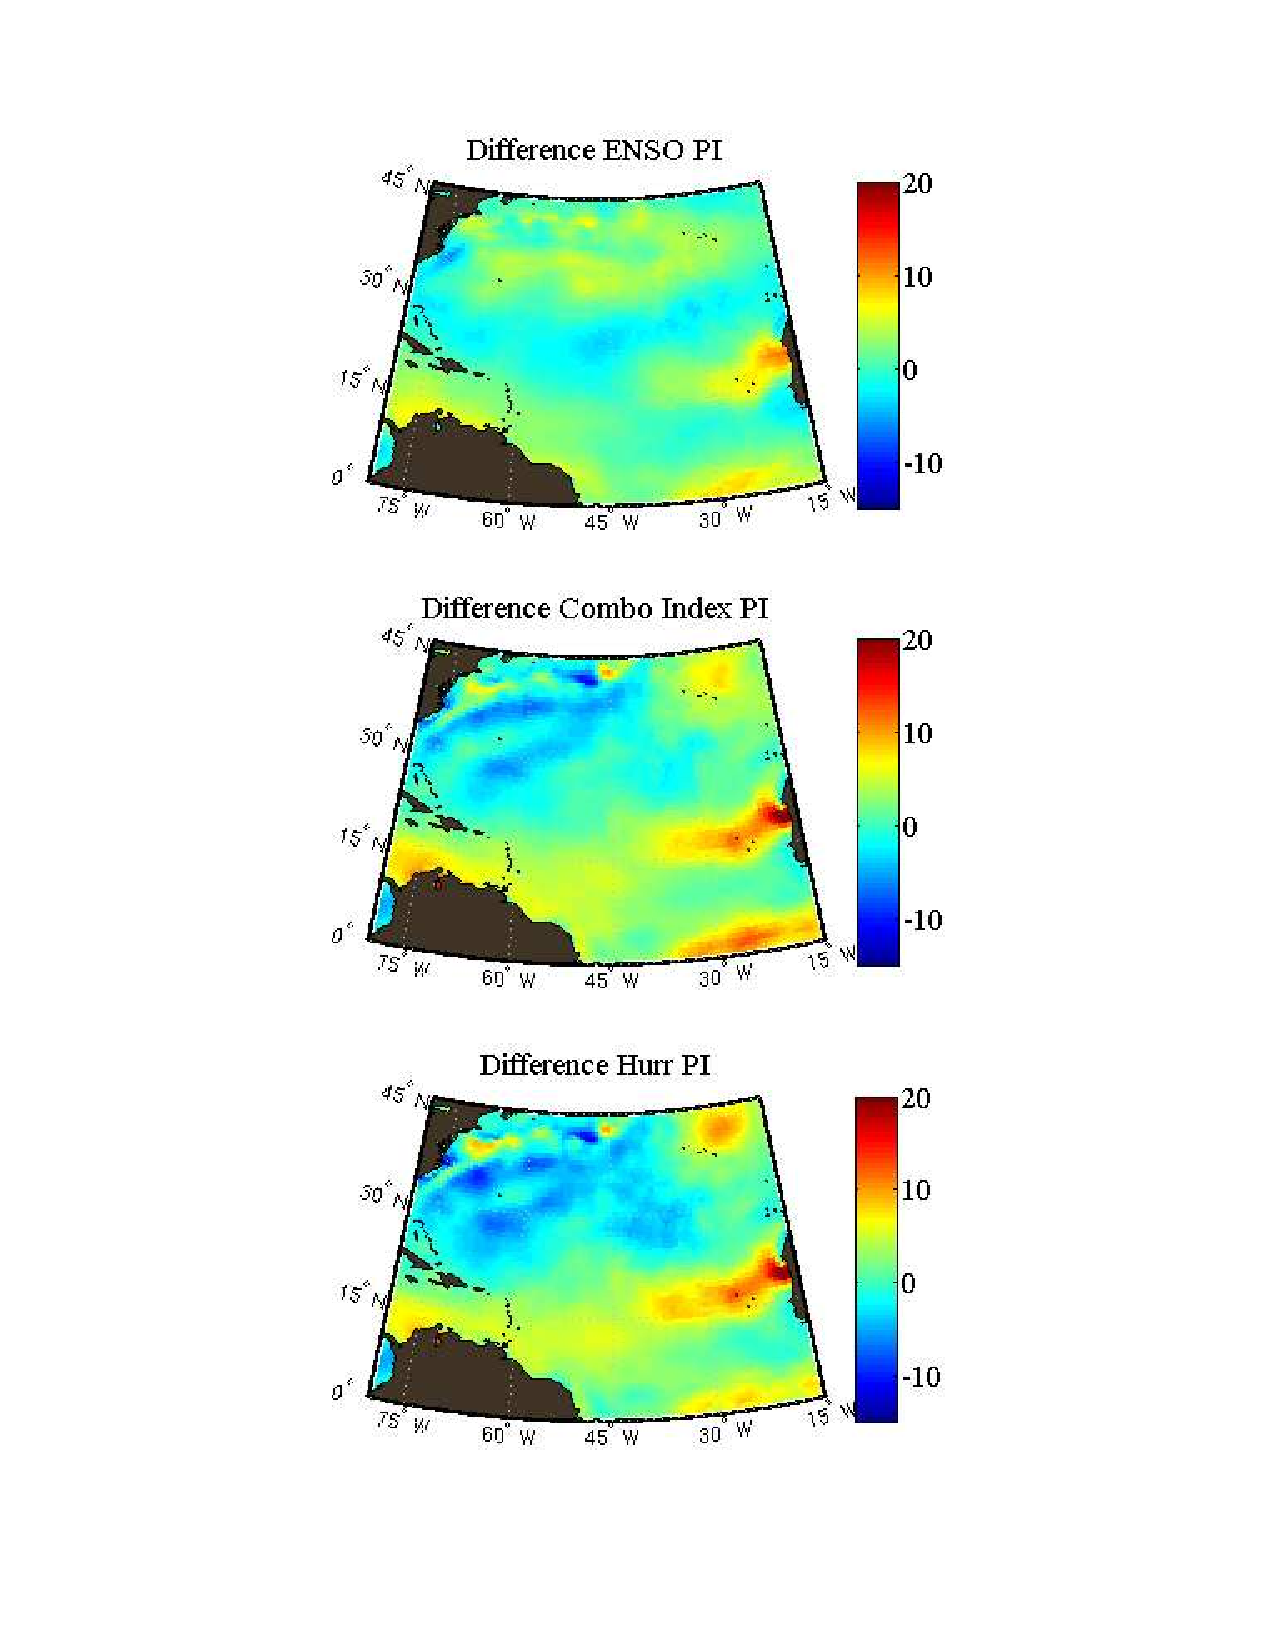
\includegraphics[width=\textwidth]{figures/comboIndex/composites/compareMDRCompositesPI.pdf}
% \caption{Central pressure composites for NINO3.4 (top), Combo Index (Middle), and Ground Truth (Bottom). Active TC seasons tend to high PI values along the MDR and right off the West African coast.}
% \label{fig:pi_comp}
% \end{minipage}
% \end{figure}
% 
% \subsubsection{Relative Humidity (RH)}
% In order for TCs to develop a minimal amount of moisture must be present in the vertical column \cite{emanuel1999}. That is why active TC seasons tend to have high RH in the East Atlantic where most hurricane form (figure \ref{fig:rh850_comp}). While our index resolves the conditions over the Atlantic better than NINO3.4 (Figure \ref{fig:rh850_comp} top), it over estimate RH in the Western Atlantic. Other moisture variables to look into are precipitable water and saturation deficit. 
% 
% \subsubsection{Sea Surface Temperatures (SST)}
% Our index is particularly better at resolving seasonal SSTs compared to NINO3.4.
% 
% \begin{figure}[ht]
% \begin{minipage}[b]{0.55\linewidth}
% 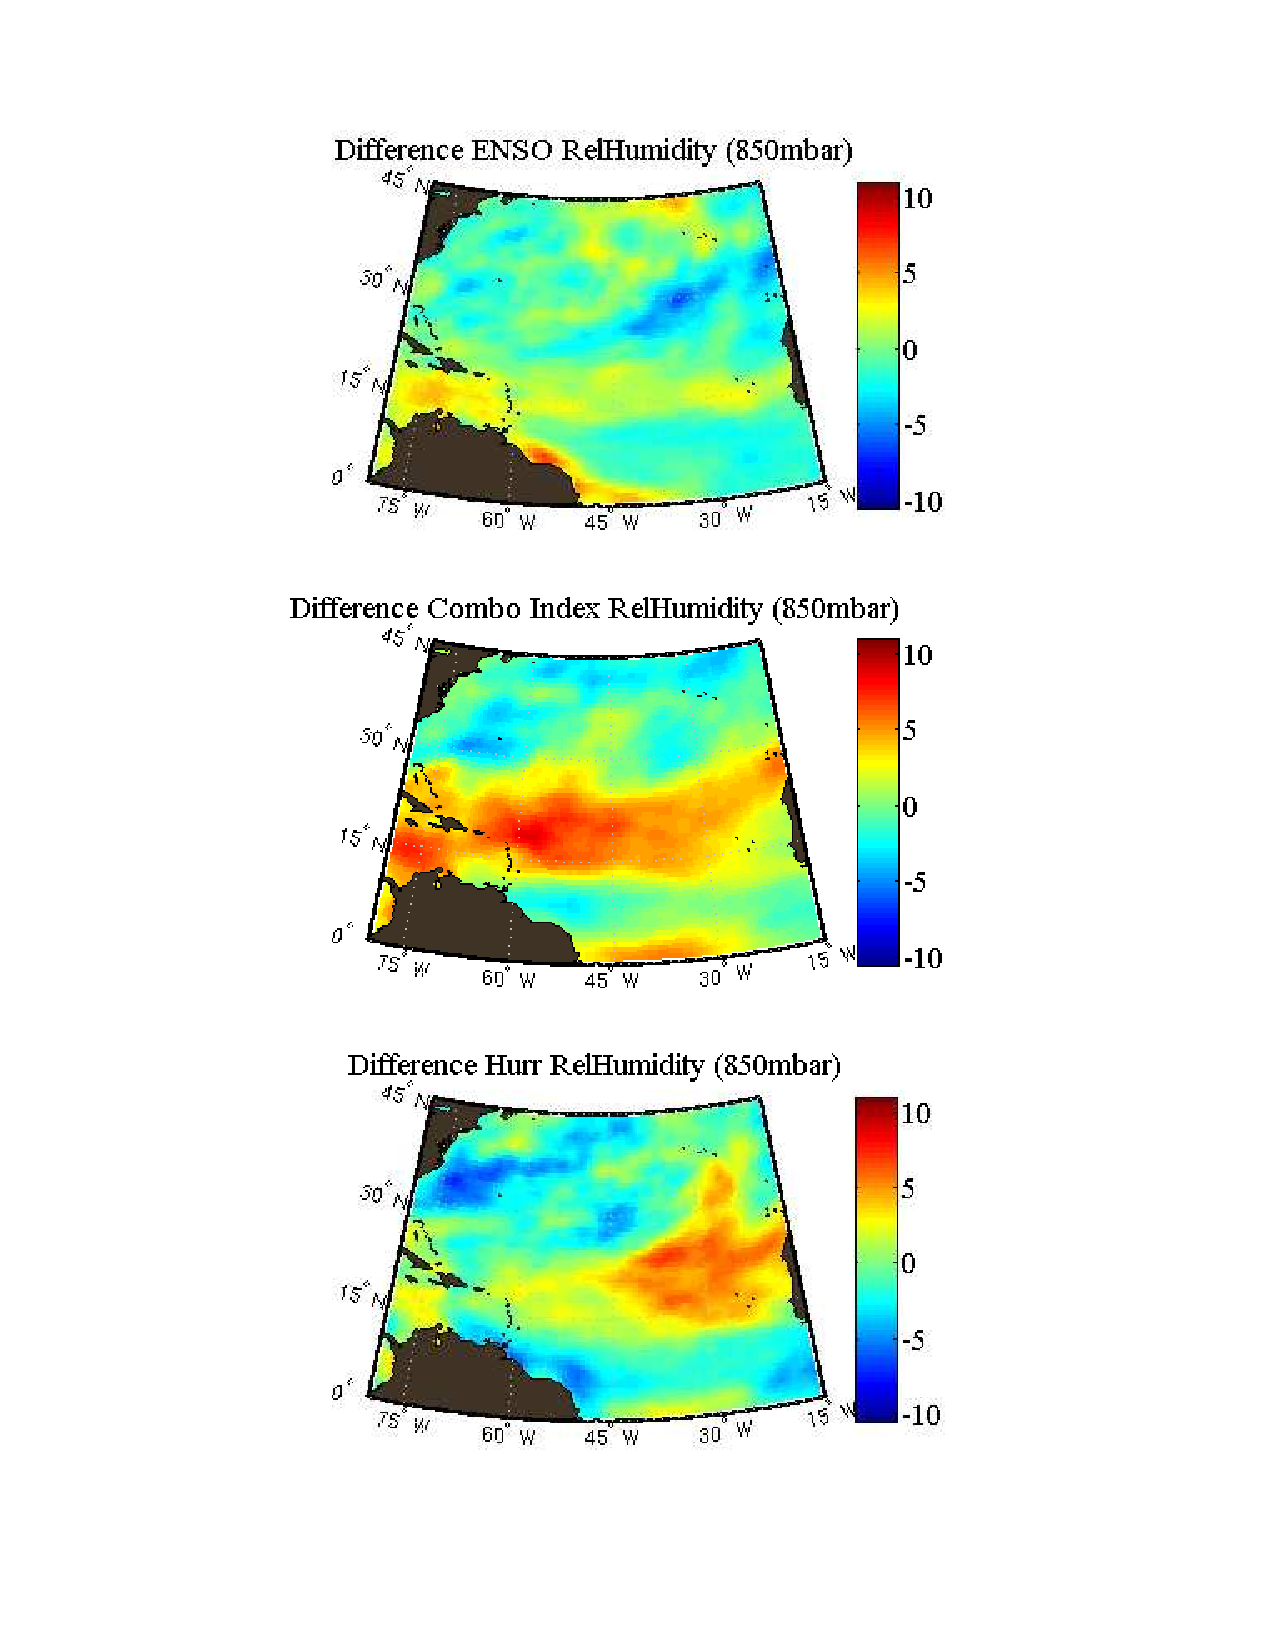
\includegraphics[width=\textwidth]{figures/comboIndex/composites/compareMDRCompositesRelativeHumidity.pdf}
% \caption{850 mb Relative Humidity composites for NINO3.4 (top), Combo Index (Middle), and Ground Truth (Bottom). Active TC seasons tend to have high RH along the MDR.}
% \label{fig:rh850_comp}
% \end{minipage}
% \hspace{0.3cm}
% \begin{minipage}[b]{0.55\linewidth}
% 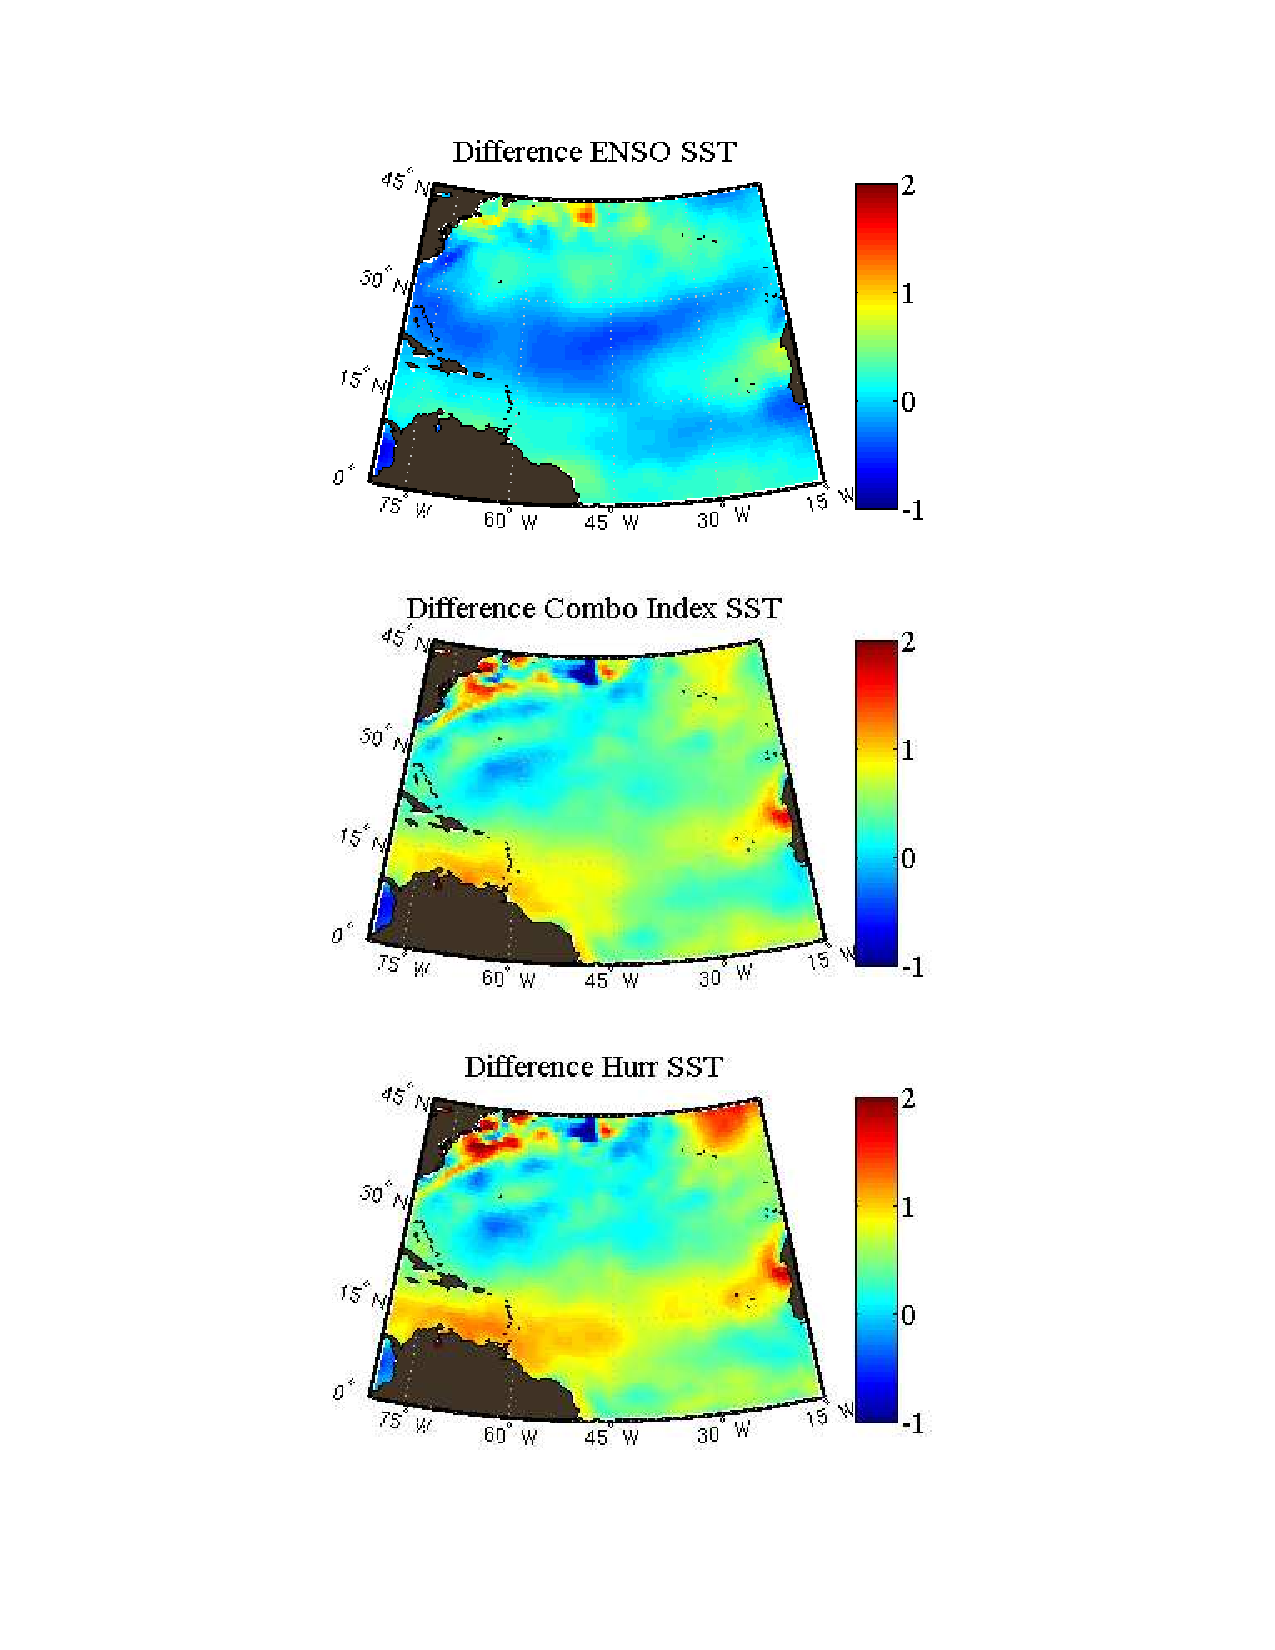
\includegraphics[width=\textwidth]{figures/comboIndex/composites/compareMDRCompositesSST.pdf}
% \caption{SST Composites for NINO3.4 (top), Combo Index (Middle), and Ground Truth (Bottom). Active TC seasons tend to have high SSTs along the MDR and in the North Atlantic.}
% \label{fig:sst_comp}
% \end{minipage}
% \end{figure}
% 
% \begin{figure}[ht]
% \begin{minipage}[b]{0.55\linewidth}
% 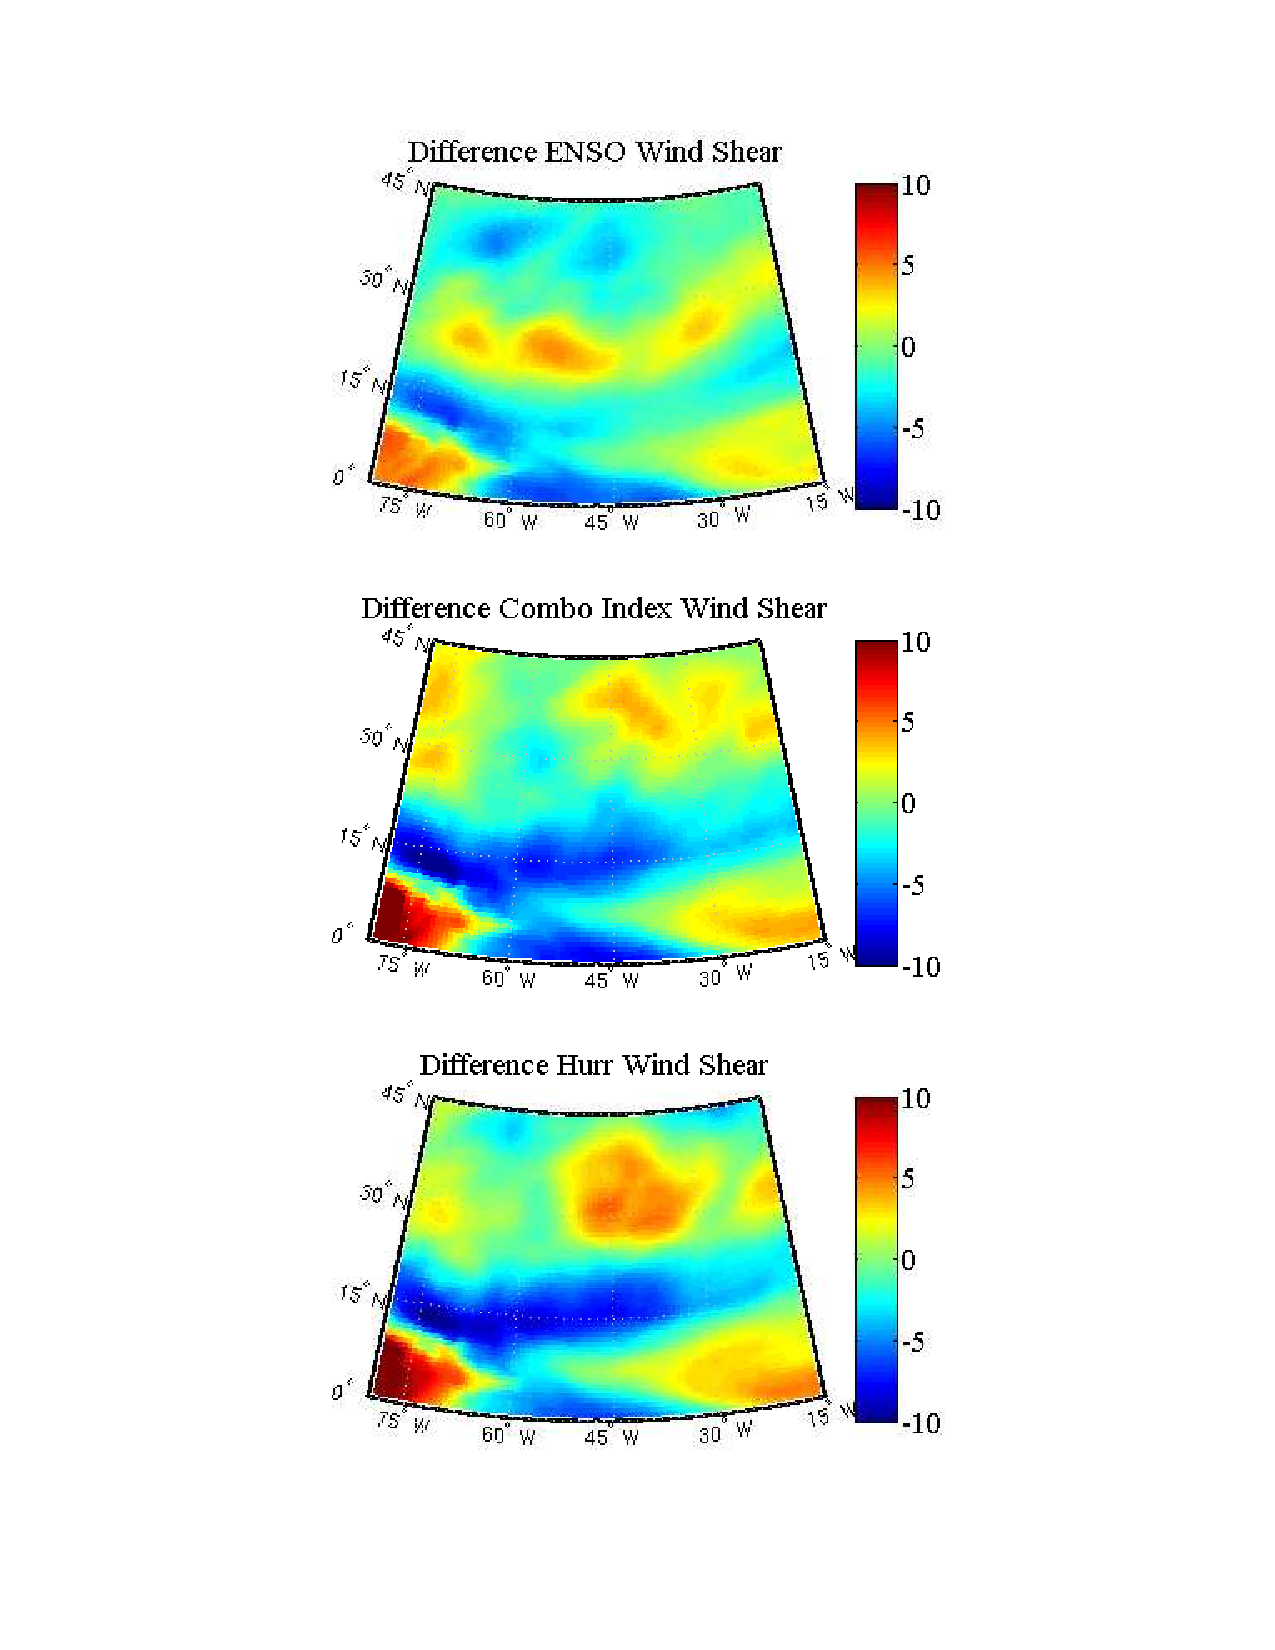
\includegraphics[width=\textwidth]{figures/comboIndex/composites/compareMDRCompositesWindShear.pdf}
% \caption{Vertical wind shear (VWS) Composites for NINO3.4 (top), Combo Index (Middle), and Ground Truth (Bottom). Active TC seasons tend to have low VWS along the MDR.}
% \label{fig:vws_comp}
% \end{minipage}
% \hspace{0cm}
% \begin{minipage}[b]{0.55\linewidth}
% %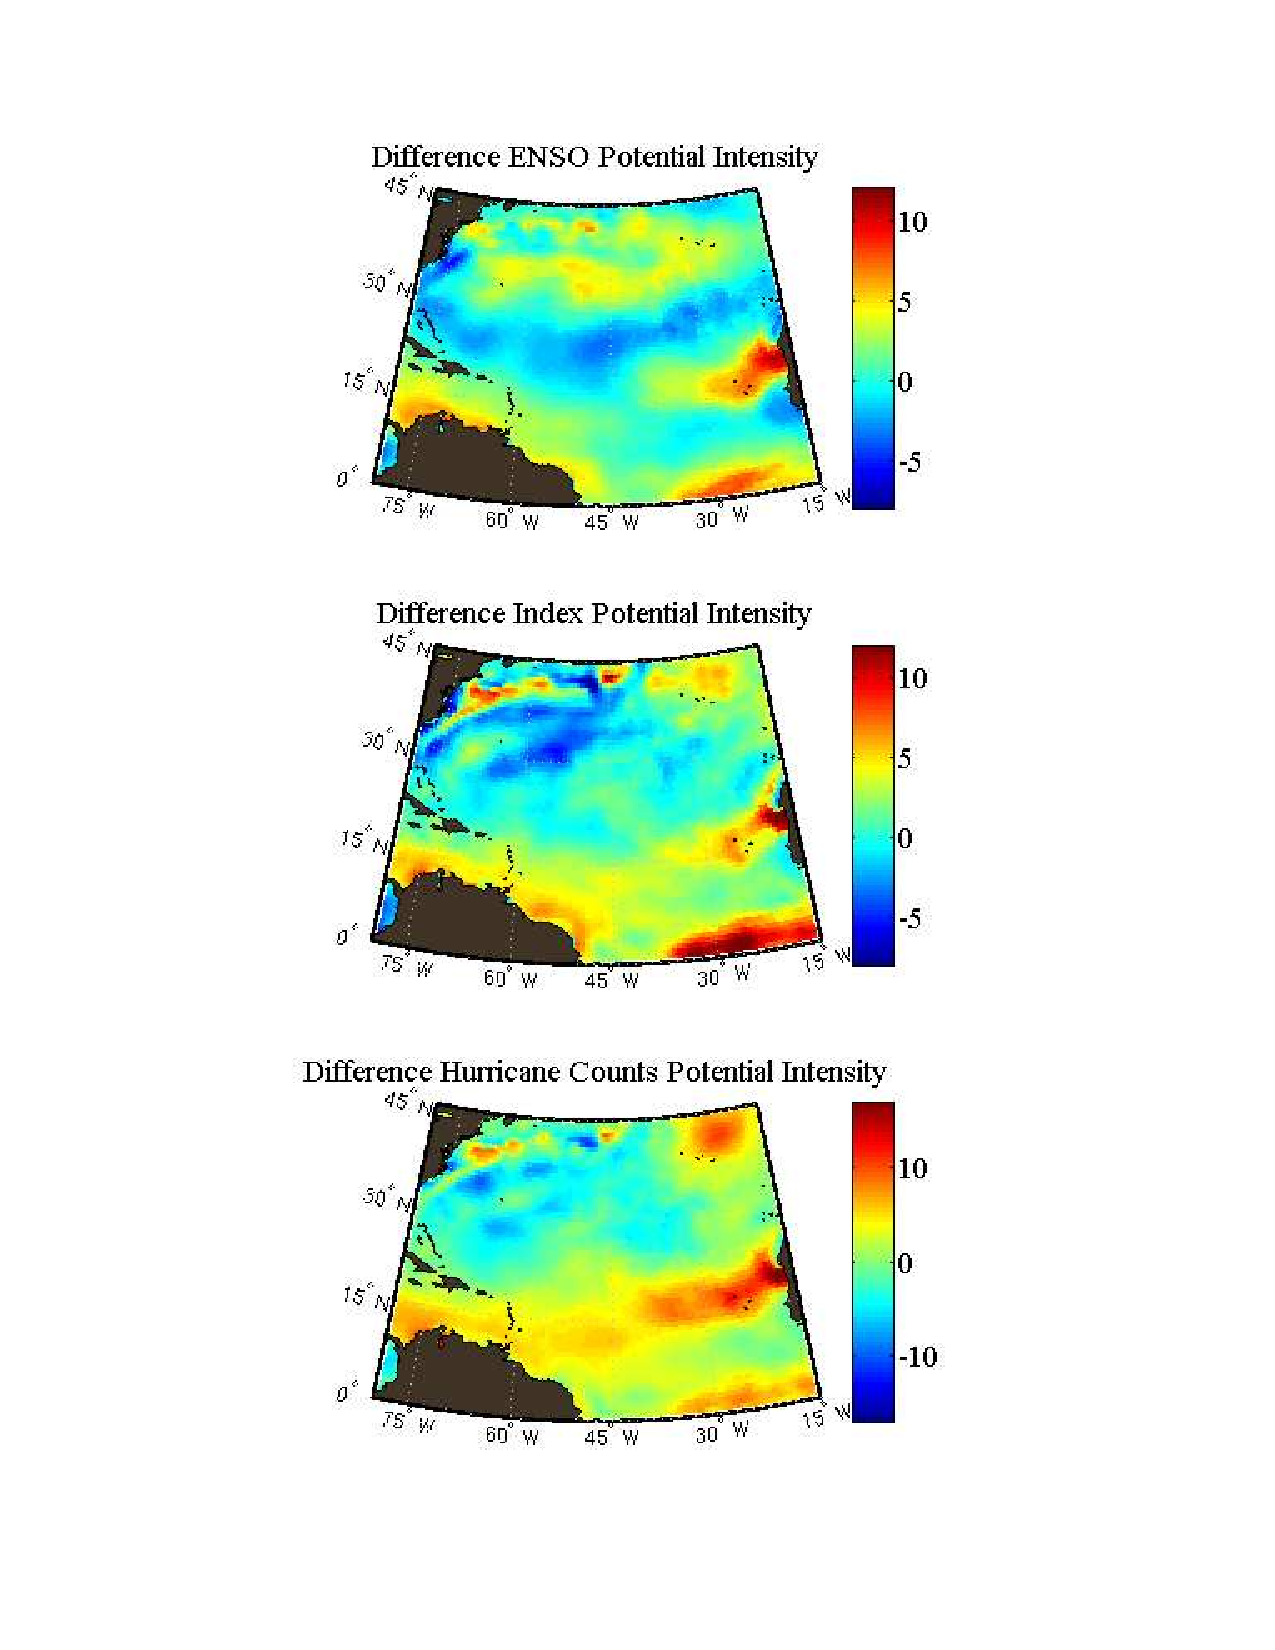
\includegraphics[width=\textwidth]{figures/sensitivityResults/compositeMaps/diffPIAtlanticComposites.pdf}
% %\caption{Diff PI Composites}
% \label{fig:figure37}
% \end{minipage}
% \end{figure}


% \clearpage
% \section{Appendix}
% \subsection{ENSO Overview}
% The quasi-periodic cycle (2-7 years) of warming and cooling of the near equatorial Pacific Ocean, known as the El-Ni\~no Souther Oscillation (ENSO) is associated with anomalous atmospheric circulation and alterations to the Eastern Pacific thermocline (the subsurface boundary between upper warm waters and deep cool waters). During its warm, El-Ni\~no (EN) phase, the equatorial Pacific Ocean experiences weak easterly winds causing an increase in Eastern Pacific SSTs, that in turn alters the atmospheric zonal (Walker) circulation, generally resulting in prevailing westerlies. ENSO's cold, La Ni\~na (LN) phase, is characterized by the opposite atmospheric conditions -- with cold SST anomalies along the Eastern Pacific and warm ones near the Western Pacific as a result of prevailing easterly winds (see Figure \ref{fig:enso_cartoon}). The mechanisms that control the reversal to the opposite LN phase are not fully understood \cite{kirtman1997,smith2012}. Recent research has suggested that to fully capture ENSO activity, it is no longer sufficient to monitor the warm and cold phases in the Eastern Pacific. Instead, warming patterns in the Central Pacific must be monitored as well \cite{ashok2007}. Warming in the Central Pacific, known as El Ni\~no Modoki, where a warm waters are surrounded by cold ones has been observed with increased frequency since the 1990s. Such changes have been attributed to anthropogenic global warming \cite{yeh2009} as well as natural climate variability \cite{wittenberg2009}.
% 
% Enhanced convection as a result of anomalous Pacific Ocean warming is associated with strong westerly upper tropospheric wind over the Caribbean basin and tropical Atlantic, resulting in low TC activity during EN events and high TC activity LN \cite{gray1984a}. Other studies have suggested that ENSO impact Atlantic TC activity via tropospheric warming \cite{tang2004}. 
% \clearpage
% \subsection{Combo Index Cross Validation Month Range Sensitivity Experiment}
% In this section we compute the combination index in the same fashion as described in the previous section.  These results are for building the index with varying month ranges, and then performing leave one-out cross validation with the combination index and 5 different hurricane statistics 

% \begin{figure}[ht]
% \begin{minipage}[b]{0.6\linewidth}
% 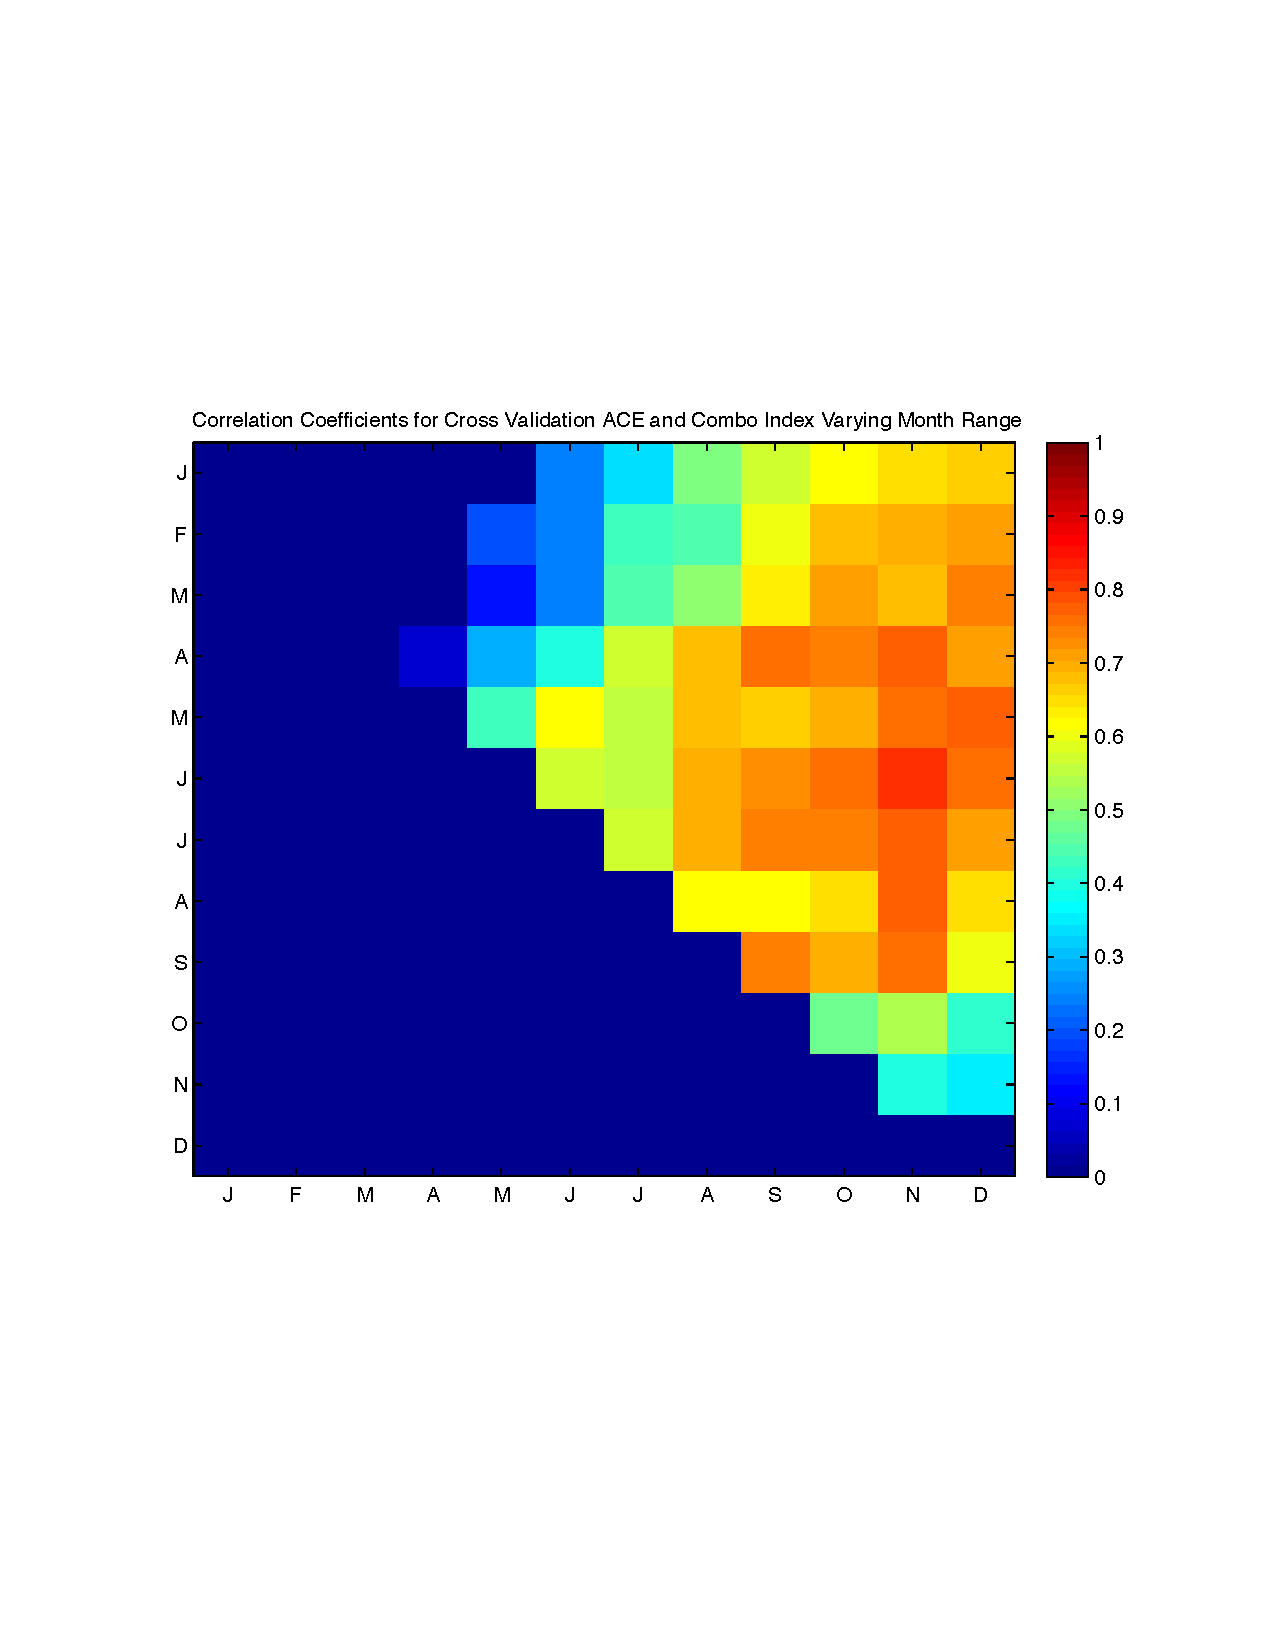
\includegraphics[width=\textwidth]{figures/comboIndex/crossValidation/monthlySensitivityTestACE.pdf}
% \caption{Corr Combo Index vs. ACE}
% \label{fig:figure38}
% \end{minipage}
% \hspace{0cm}
% \begin{minipage}[b]{0.6\linewidth}
% 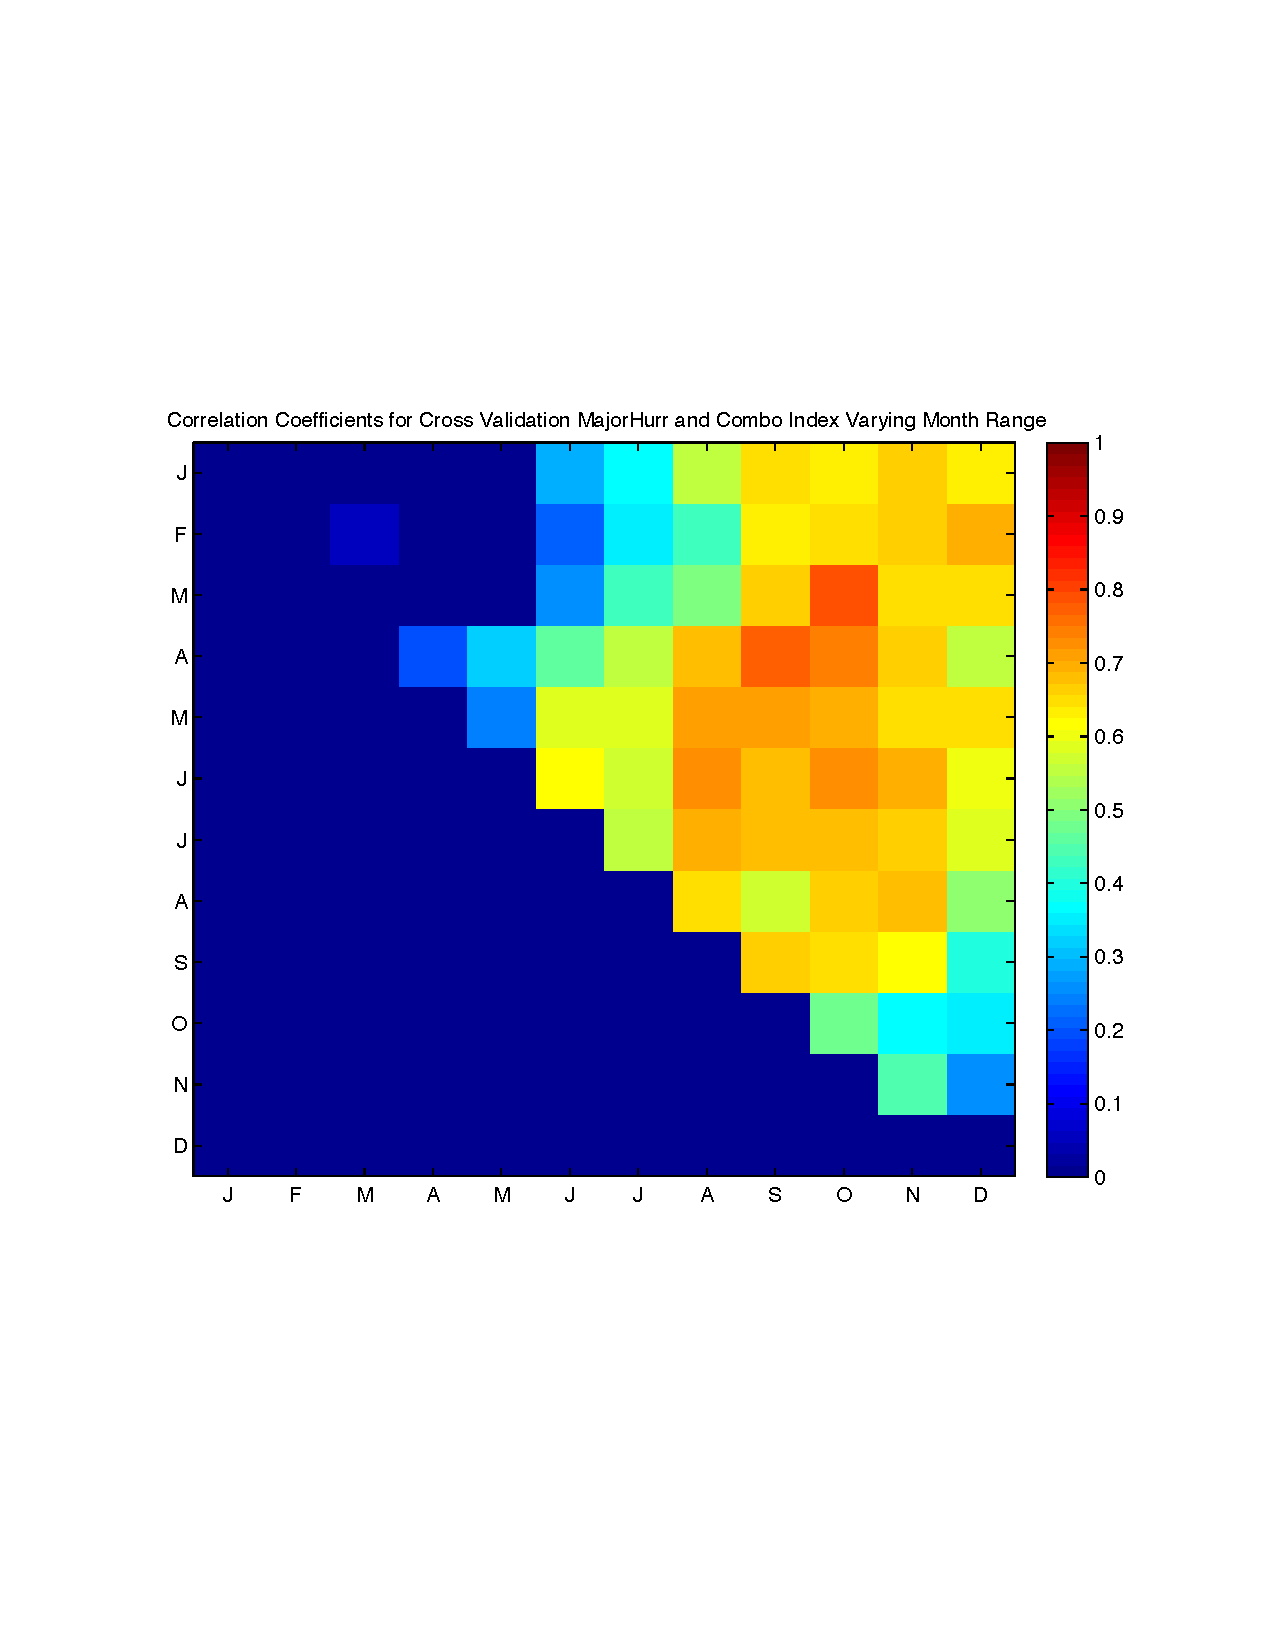
\includegraphics[width=\textwidth]{figures/comboIndex/crossValidation/monthlySensitivityTestMajorHurr.pdf}
% \caption{Corr Combo Index vs. Major Hurr}
% \label{fig:figure38}
% \end{minipage}
% \end{figure}
% 
% \begin{figure}[ht]
% \begin{minipage}[b]{0.6\linewidth}
% 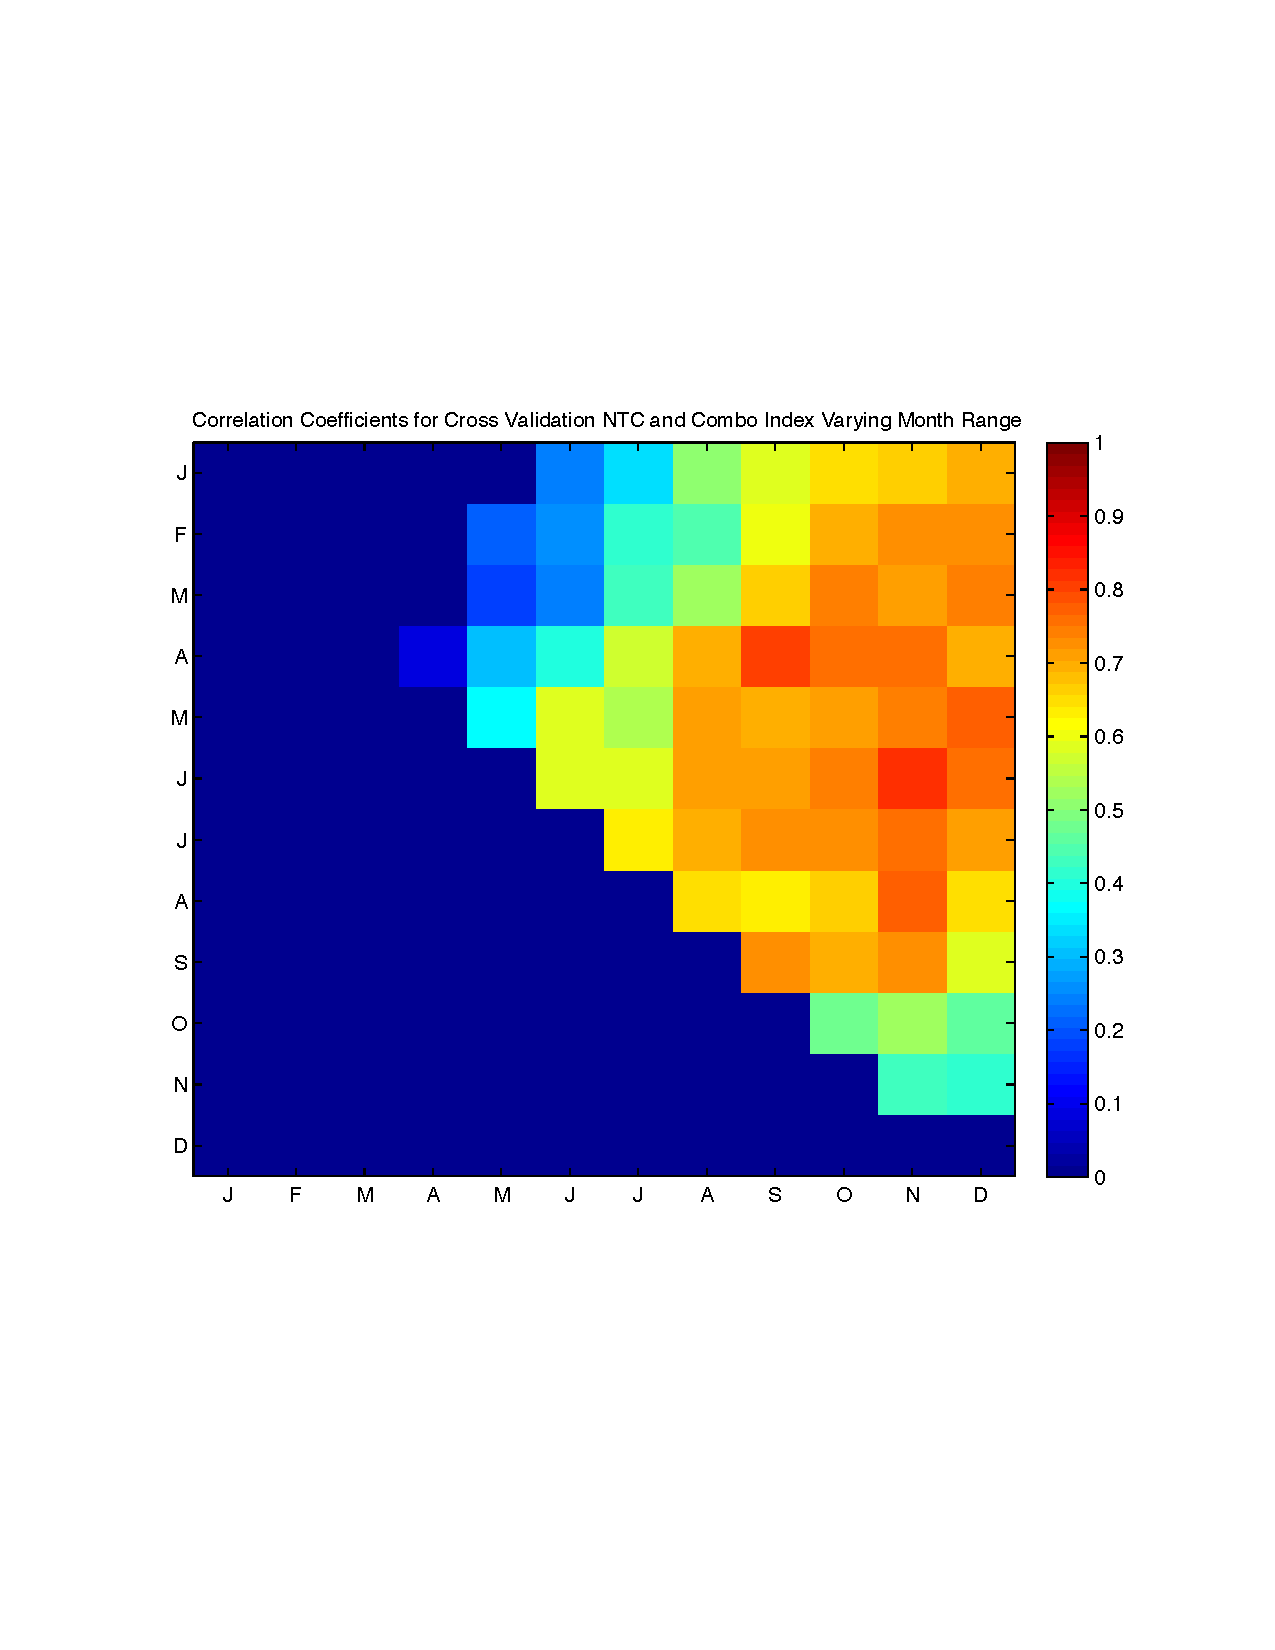
\includegraphics[width=\textwidth]{figures/comboIndex/crossValidation/monthlySensitivityTestNTC.pdf}
% \caption{Corr Combo Index vs. NTC}
% \label{fig:figure39}
% \end{minipage}
% \hspace{0cm}
% \begin{minipage}[b]{0.6\linewidth}
% 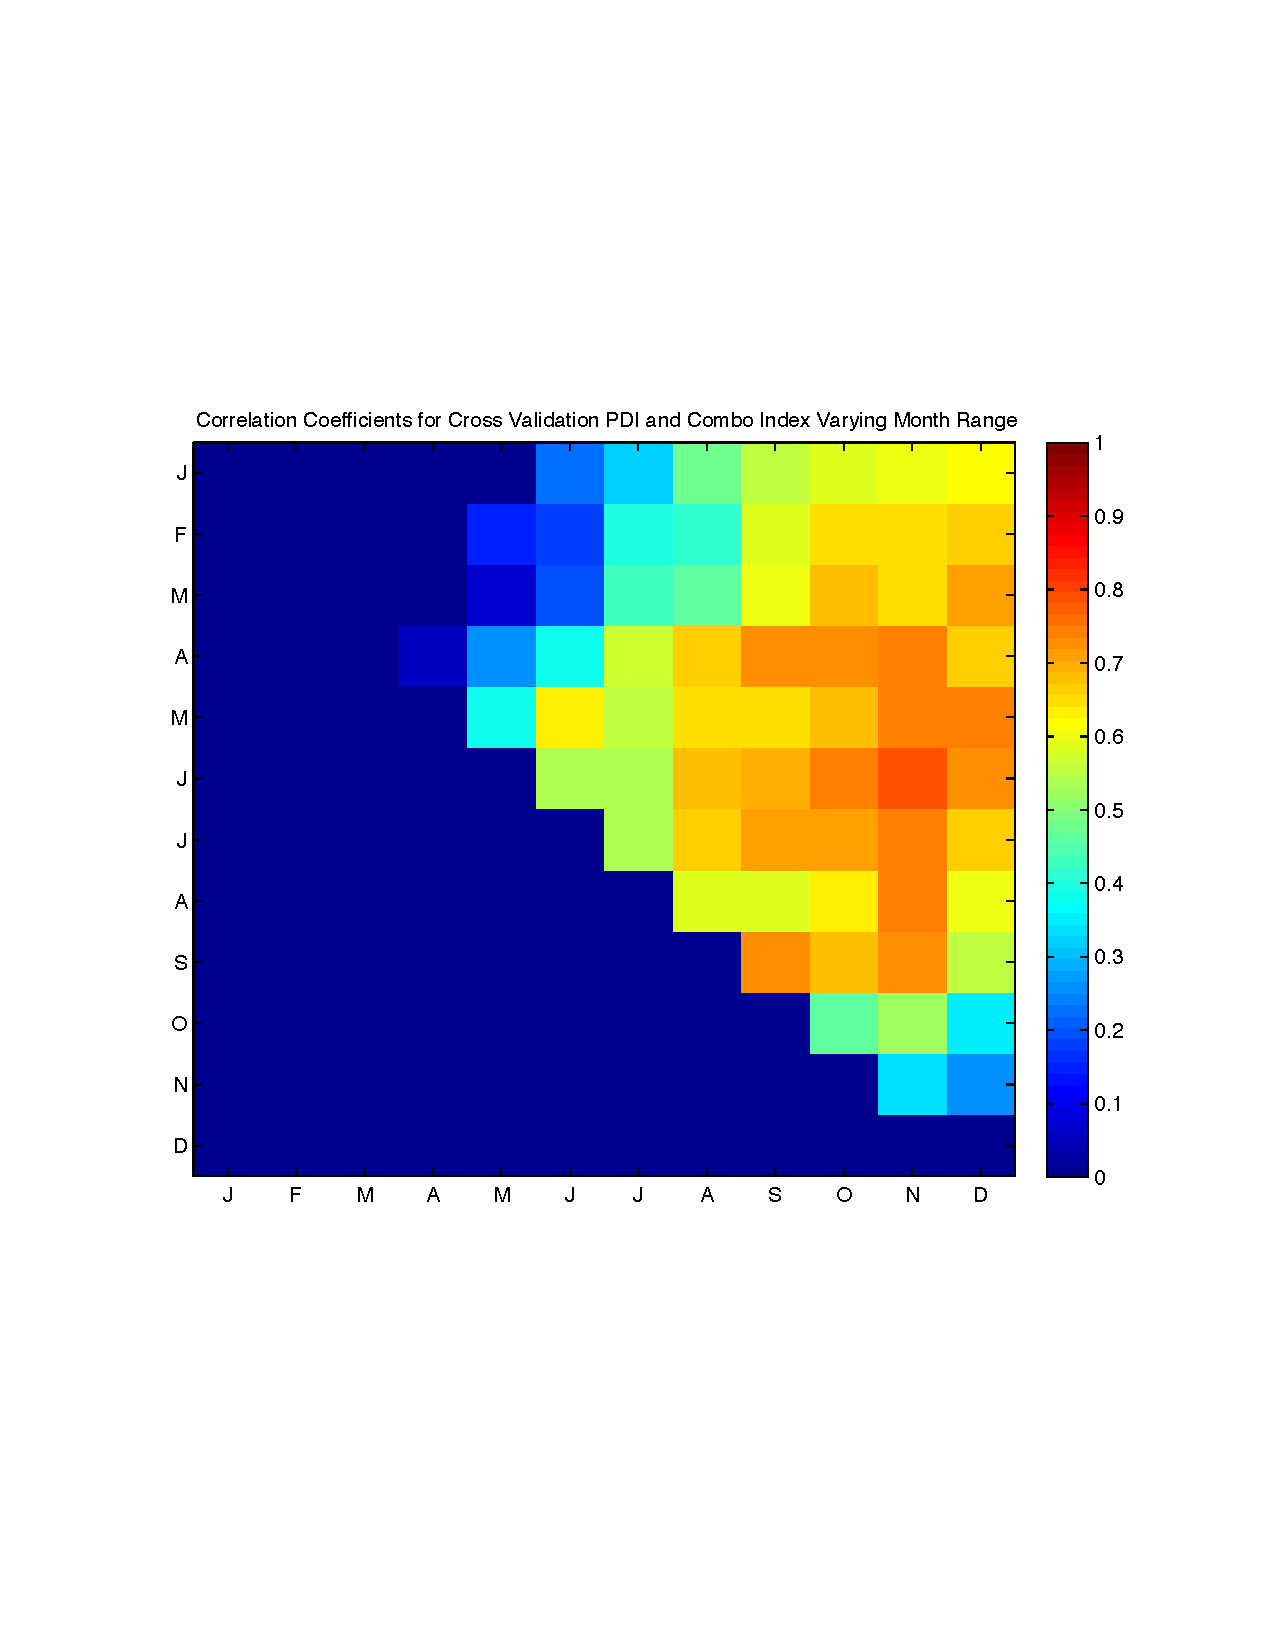
\includegraphics[width=\textwidth]{figures/comboIndex/crossValidation/monthlySensitivityTestPDI.pdf}
% \caption{Corr Combo Index vs. PDI}
% \label{fig:figure40}
% \end{minipage}
% \end{figure}
% 
% \begin{figure}[ht]
% \begin{minipage}[b]{0.6\linewidth}
% 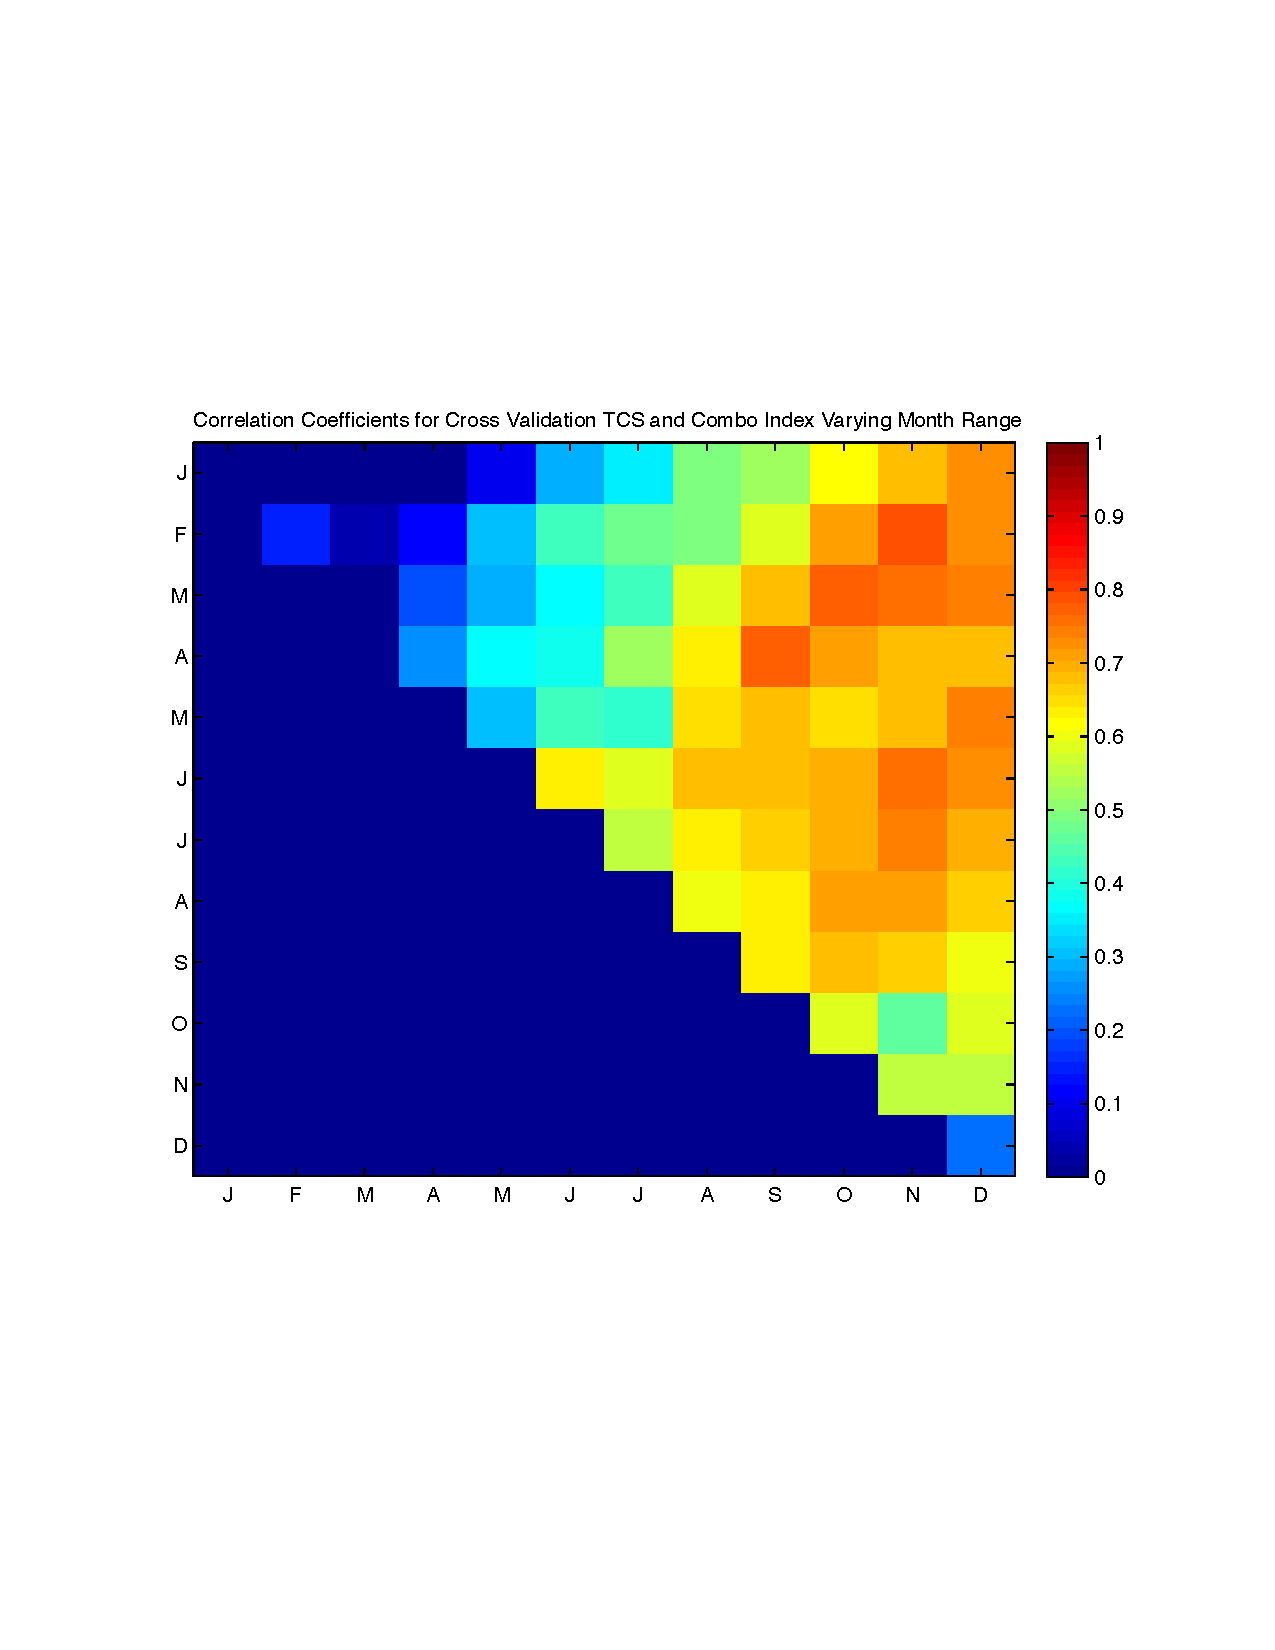
\includegraphics[width=\textwidth]{figures/comboIndex/crossValidation/monthlySensitivityTestTCS.pdf}
% \caption{Corr Combo Index vs. TCs}
% \label{fig:figure41}
% \end{minipage}
% \hspace{0cm}
% \begin{minipage}[b]{0.6\linewidth}
% %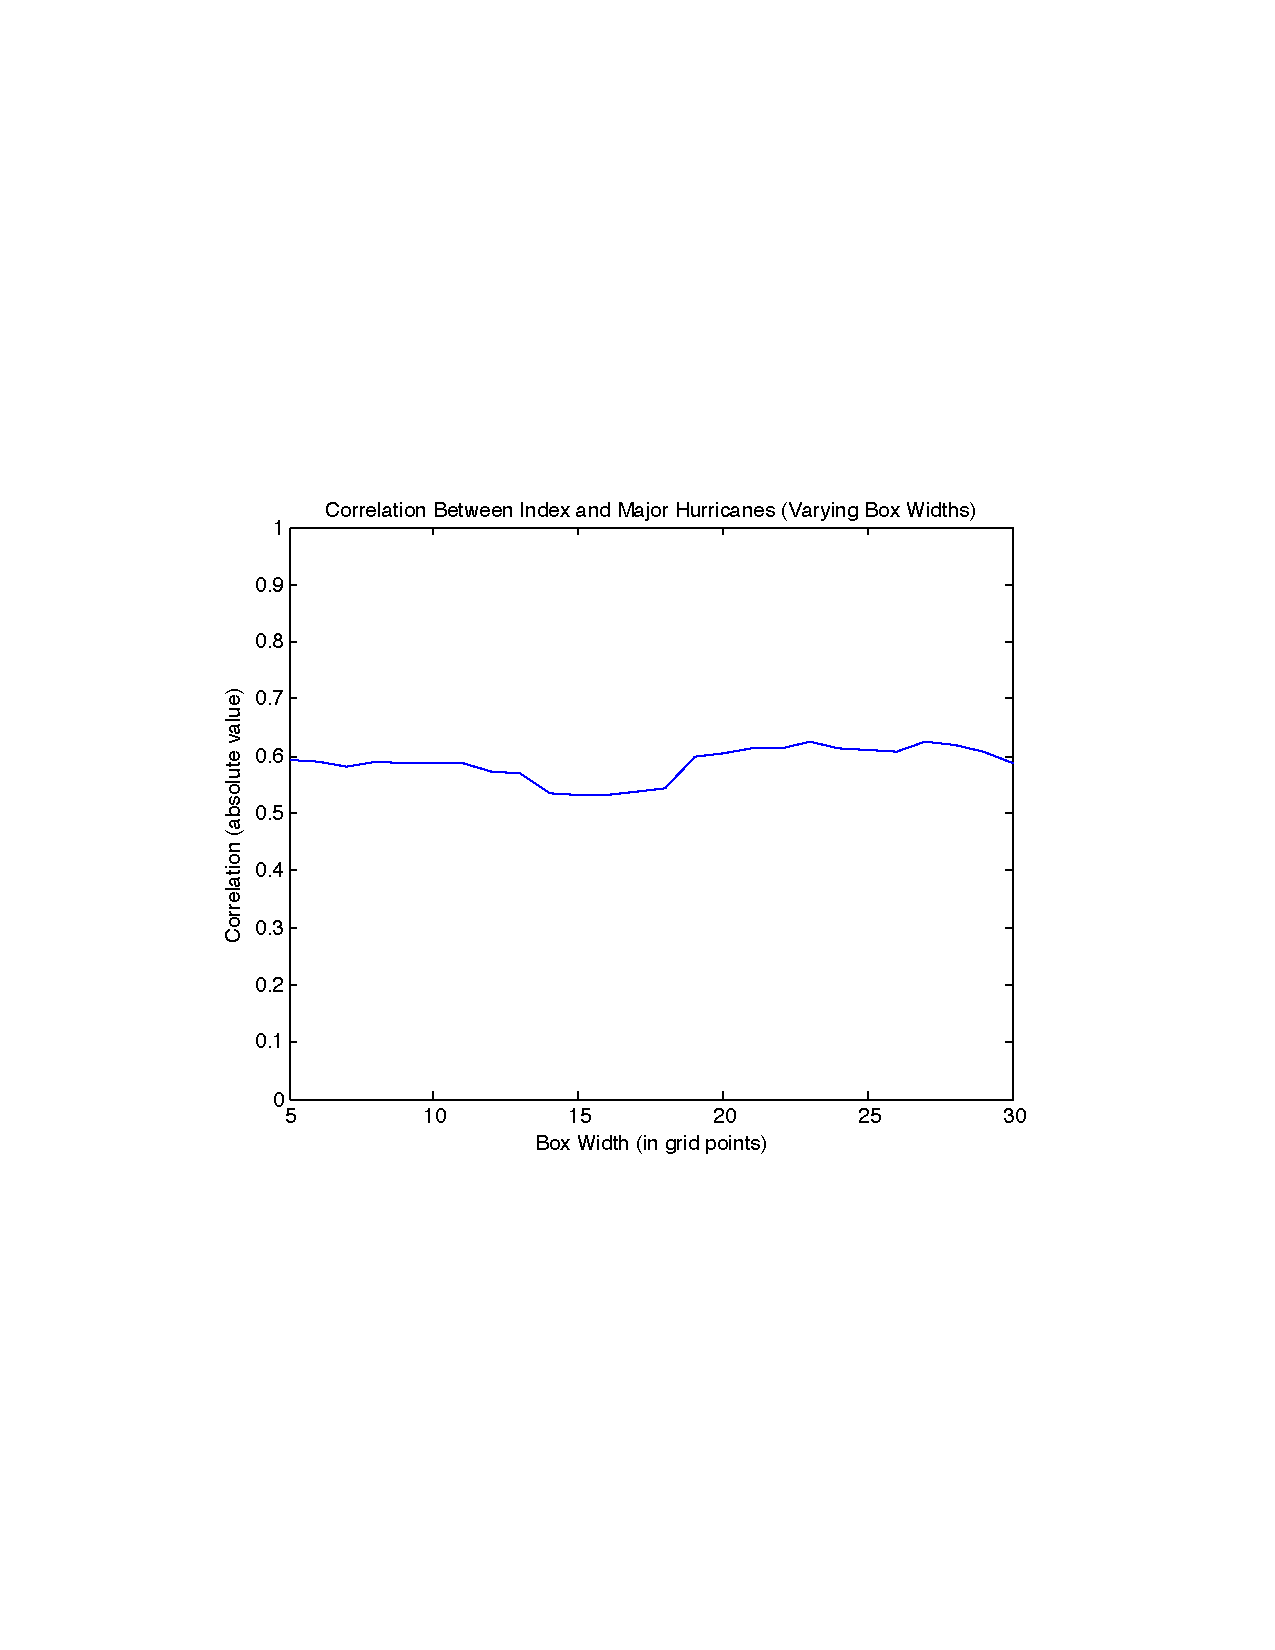
\includegraphics[width=\textwidth]{figures/sensitivityResults/boxSize/Major_Hurricanes_Index_Box_Size.pdf}
% %\caption{Corr Index vs. Major Hurricanes}
% %\label{fig:figure2}
% \end{minipage}
% \end{figure}

%In fact, recent research has attributed increased accuracy in predicting seasonal TC activity with reasonable lead times to an increased ability to predict Pacific SSTs \cite{smith2010}.$

%The warming anomalies of sea surface temperatures (SSTs) along the near-equatorial Pacific Ocean have well documented global long-range weather teleconnections from rainfall in southern India to mudslides in the western United States. 

% Hurricanes, or more generally tropical cyclones (TCs), are one of the most devastating natural disasters in terms of both human and material loss. Therefore there is significant scientific and societal interest in understanding how will TC activity (frequency, intensity, and trajectories) evolve especially under global warming conditions. Our understanding our future TC activity under various warming scenarios is limited \cite{knutson2010} mainly due to two major questions: First, how will the large scale conditions over TC development regions evolve if the environment continues to warm; (ii) and if we can predict such conditions what would future TC activity be as a response to such large-scale changes? Subsequently, to understand future Atlantic TC activity, we must first understand how will the large-scale conditions over the Atlantic change and how will Atlantic TCs respond to such changes.


% 
% \begin{figure}[htbp]
% 	\centering
% 		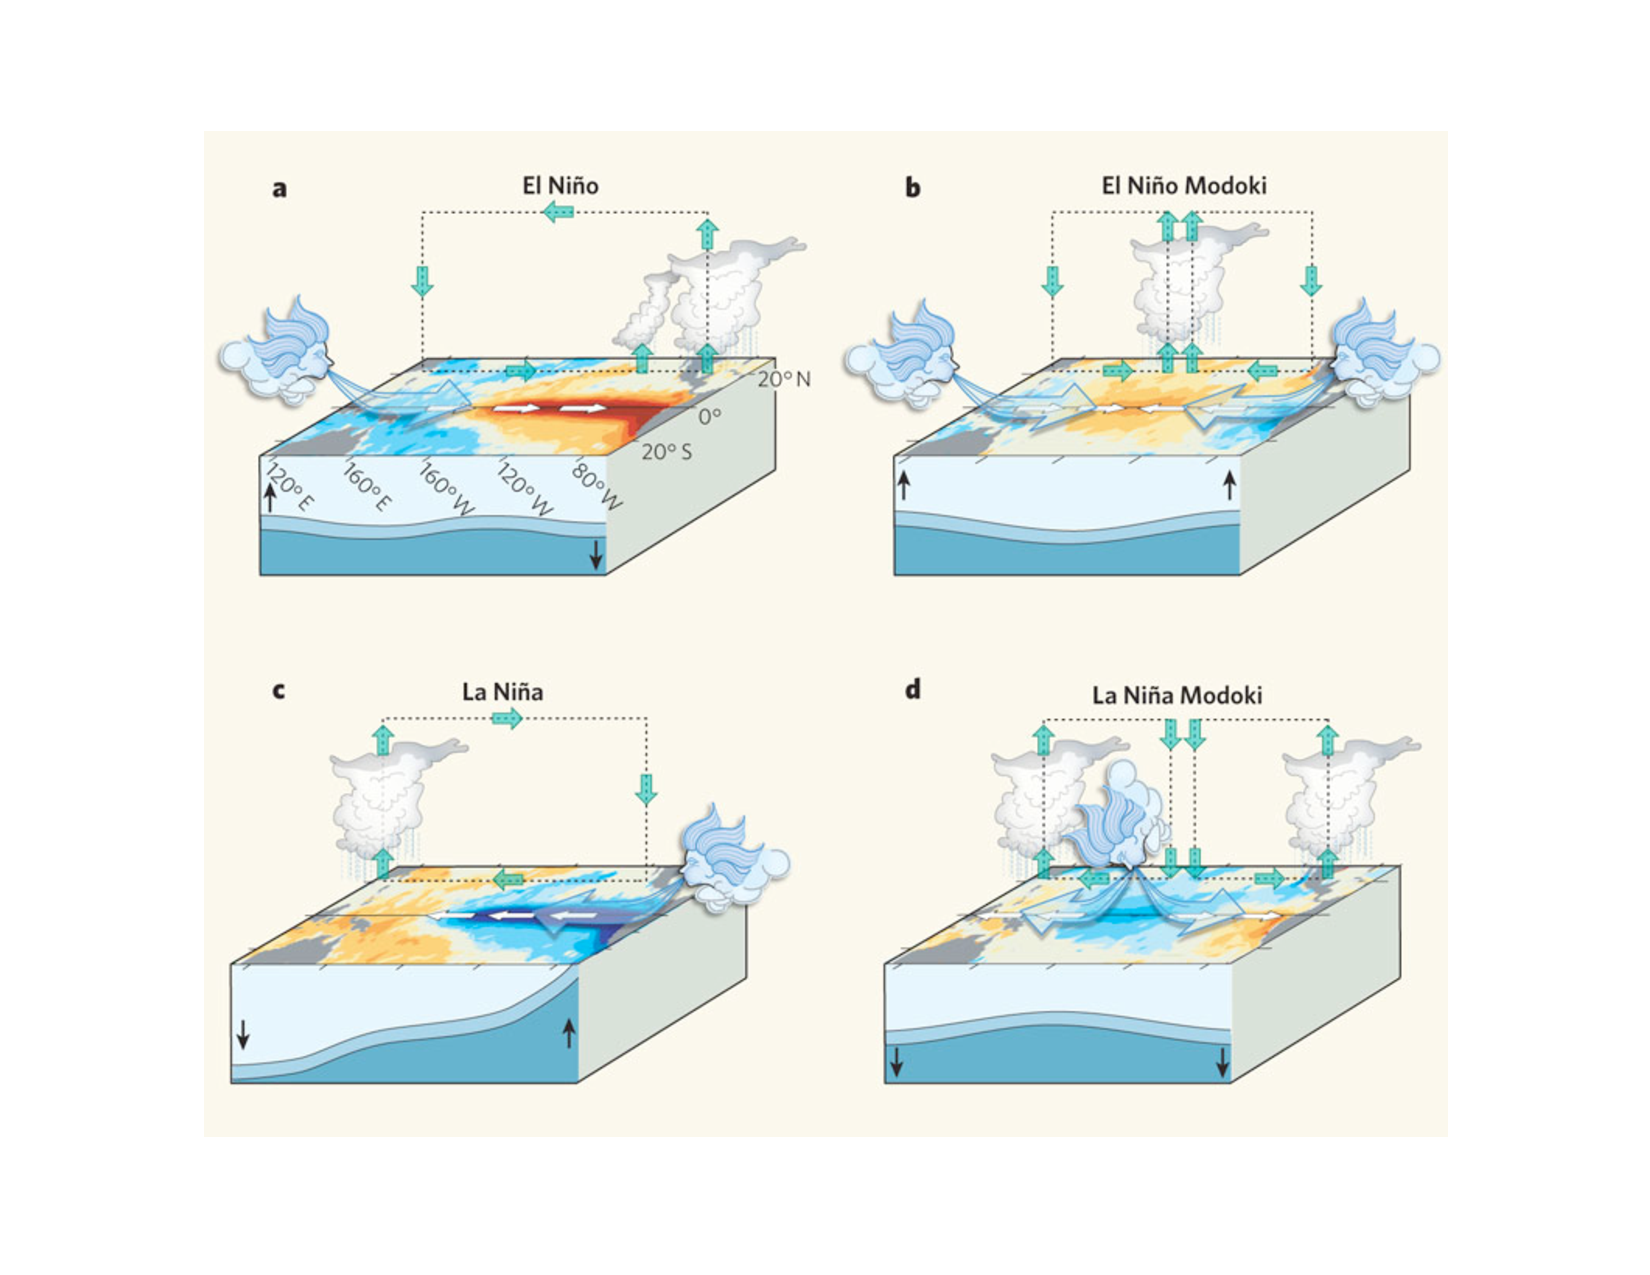
\includegraphics[height=2.5in]{figures/nino_cartoon.pdf}
% 	\caption{(a), An El Ni\~no event is produced when the easterly winds weaken; sometimes, in the west, westerlies prevail. This condition is categorized by warmer than normal sea surface temperatures (SSTs) in the east of the ocean, and is associated with alterations in the thermocline and in the atmospheric circulation that make the east wetter and the west drier. (b), An El Ni\~no Modoki event is an anomalous condition of a distinctly different kind. The warmest SSTs occur in the central Pacific, flanked by colder waters to the east and west, and are associated with distinct patterns of atmospheric convection. (c), (d), The opposite (La Ni\~na) phases of the El Niño and El Ni\~no Modoki respectively. Image and caption used for illustration purposes only taken from \cite{ashok2009}}
% 	\label{fig:enso_cartoon}
% \end{figure}

%Tables \ref{table:april_lead} through \ref{table:oct_lead} show the linear correlation coefficients between August-October TC Atlantic TC activity and our ENSO spatial index for Feb-April, April-June, and August-October respectively. In all cases our spatial ENSO index correlates better than traditional warming-based indices. The improvements increase as we increase lead time, with April lead times improving by more than an order of magnitude. This improvement is because traditional ENSO indices suffer from a ``predictability barrier" that make it difficult to use them to predict TC activity before June \cite{webster1992}.

% \begin{table}
% \begin{center}
% \begin{tabular}{cccccc}
% \hline
% &TCs & Major Hurricanes & ACE & PDI & NTC\\
% \hline
% Spatial ENSO & -0.44 & -0.39 & -0.40 & -0.39 & -0.43\\
% NINO 1+2 & -0.07 & -0.13 & 0.01 & 0.02 & -0.04\\
% NINO 3.4 & -0.07 & -0.11 & 0.01 & 0.02 & 0.03\\
% NINO 3 & 0.04 & -0.08 & 0.06 & 0.08 & 0.03\\
% NINO 4 & 0.09 & -0.08 & 0.08 & 0.11 & 0.10\\
% \hline
% \end{tabular}
% \end{center}
% \caption{Linear correlation coefficients between January-April mean SSTs of traditional warming-based ENSO indices as well as the January-April Spatial ENSO index and August-October Atlantic TC activity. Our Spatial ENSO index significantly outperforms traditional indices.}
% \label{ref:table_jan_apl_corr}
% \end{table}
% 
% \begin{table}
% \begin{center}
% \begin{tabular}{cccccc}
% \hline
% &TCs & Major Hurricanes & ACE & PDI & NTC\\
% \hline
% Spatial ENSO & -0.53 & -0.48 & -0.36 & -0.34 & -0.40\\
% NINO 1+2 & -0.23 & -0.32 & -0.25 & -0.26 & -0.28\\
% NINO 3.4 & -0.23 & -0.44 & -0.25 & -0.26 & -0.29\\
% NINO 3 & -0.28 & -0.40 & -0.28 & -0.29 & -0.31\\
% NINO 4 & -0.10 & -0.27 & -0.10 & -0.08 & -0.09\\
% \hline
% \end{tabular}
% \end{center}
% \caption{Linear correlation coefficients between April-June mean SSTs of traditional warming-based ENSO indices as well as the January-April Spatial ENSO index and August-October Atlantic TC activity. Our Spatial ENSO index significantly outperforms traditional indices.}
% \label{ref:table_apr_jun}
% \end{table}
% 
% \begin{table}
% \begin{center}
% \begin{tabular}{cccccc}
% \hline
% &TCs & Major Hurricanes & ACE & PDI & NTC\\
% \hline
% Spatial ENSO & -0.62 & -0.57 & -0.69 & -0.67 & -0.70\\
% NINO 1+2 & -0.55 & -0.47 & -0.44 & -0.42 & -0.49\\
% NINO 3.4 & -0.55 & -0.51 & -0.44 & -0.42 & -0.46\\
% NINO 3 & -0.51 & -0.50 & -0.46 & -0.44 & -0.49\\
% NINO 4 & -0.34 & -0.48 & -0.33 & -0.32 & -0.35\\
% \hline
% \end{tabular}
% \end{center}
% \caption{Linear correlation coefficients between July-October mean SSTs of traditional warming-based ENSO indices as well as the January-April Spatial ENSO index and August-October Atlantic TC activity. Our Spatial ENSO index significantly outperforms traditional indices.}
% \label{ref:table_jul_oct}
% \end{table}
\begin{comment}
\subsection{Sensitivity Tests}
To validate our results, we test the sensitivity of our results to the month ranges used to build the index, the size of the ENSO box used, the size of the search space, and the months used as TC season. As it can be seen from the figures below, our results are stable with respect to parameter choice, except for search space where the correlations chance drastically based on which region we search.
%\pagebreak
\subsection{Box Size Sensitivity Results}

\begin{figure}[ht]
\begin{minipage}[b]{0.6\linewidth}
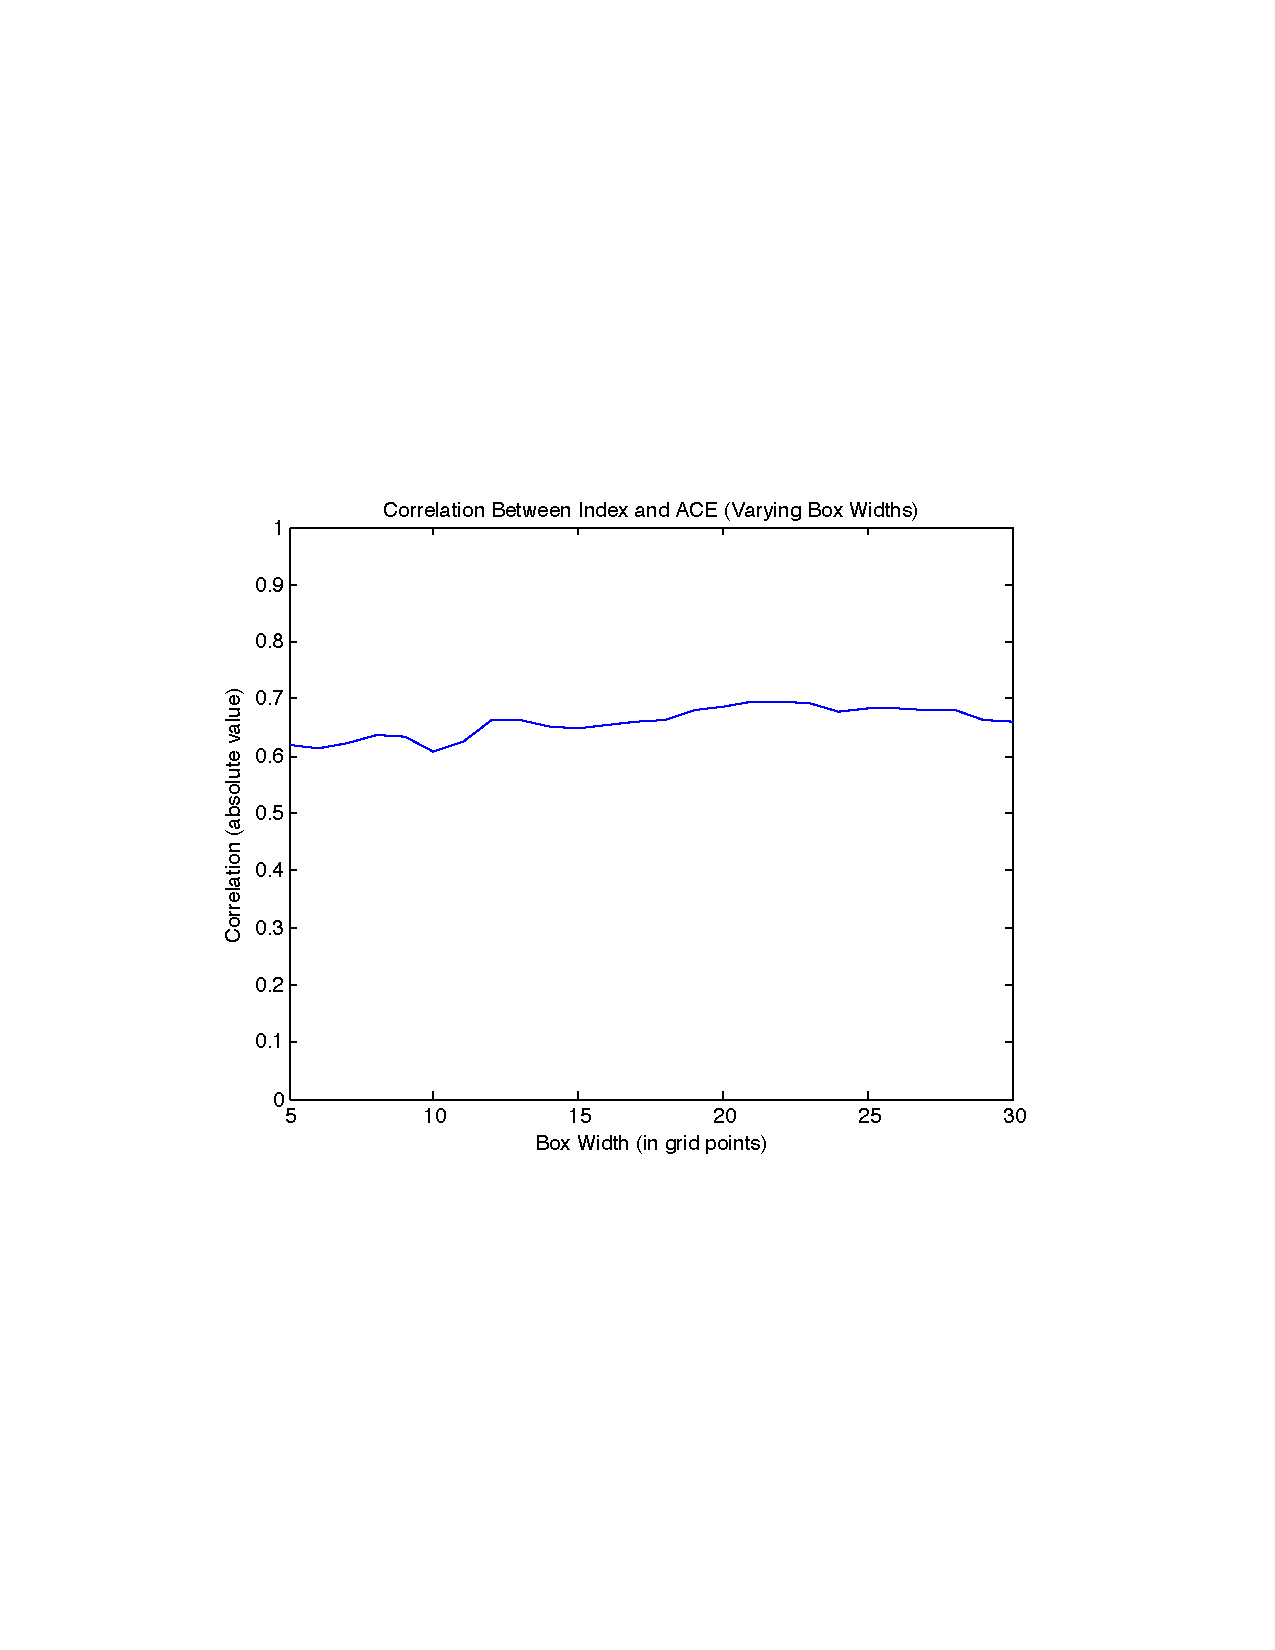
\includegraphics[width=\textwidth]{figures/sensitivityResults/boxSize/ACE_Index_Box_Size.pdf}
\caption{Corr Index vs. ACE}
\label{fig:figure1}
\end{minipage}
\hspace{0cm}
\begin{minipage}[b]{0.6\linewidth}
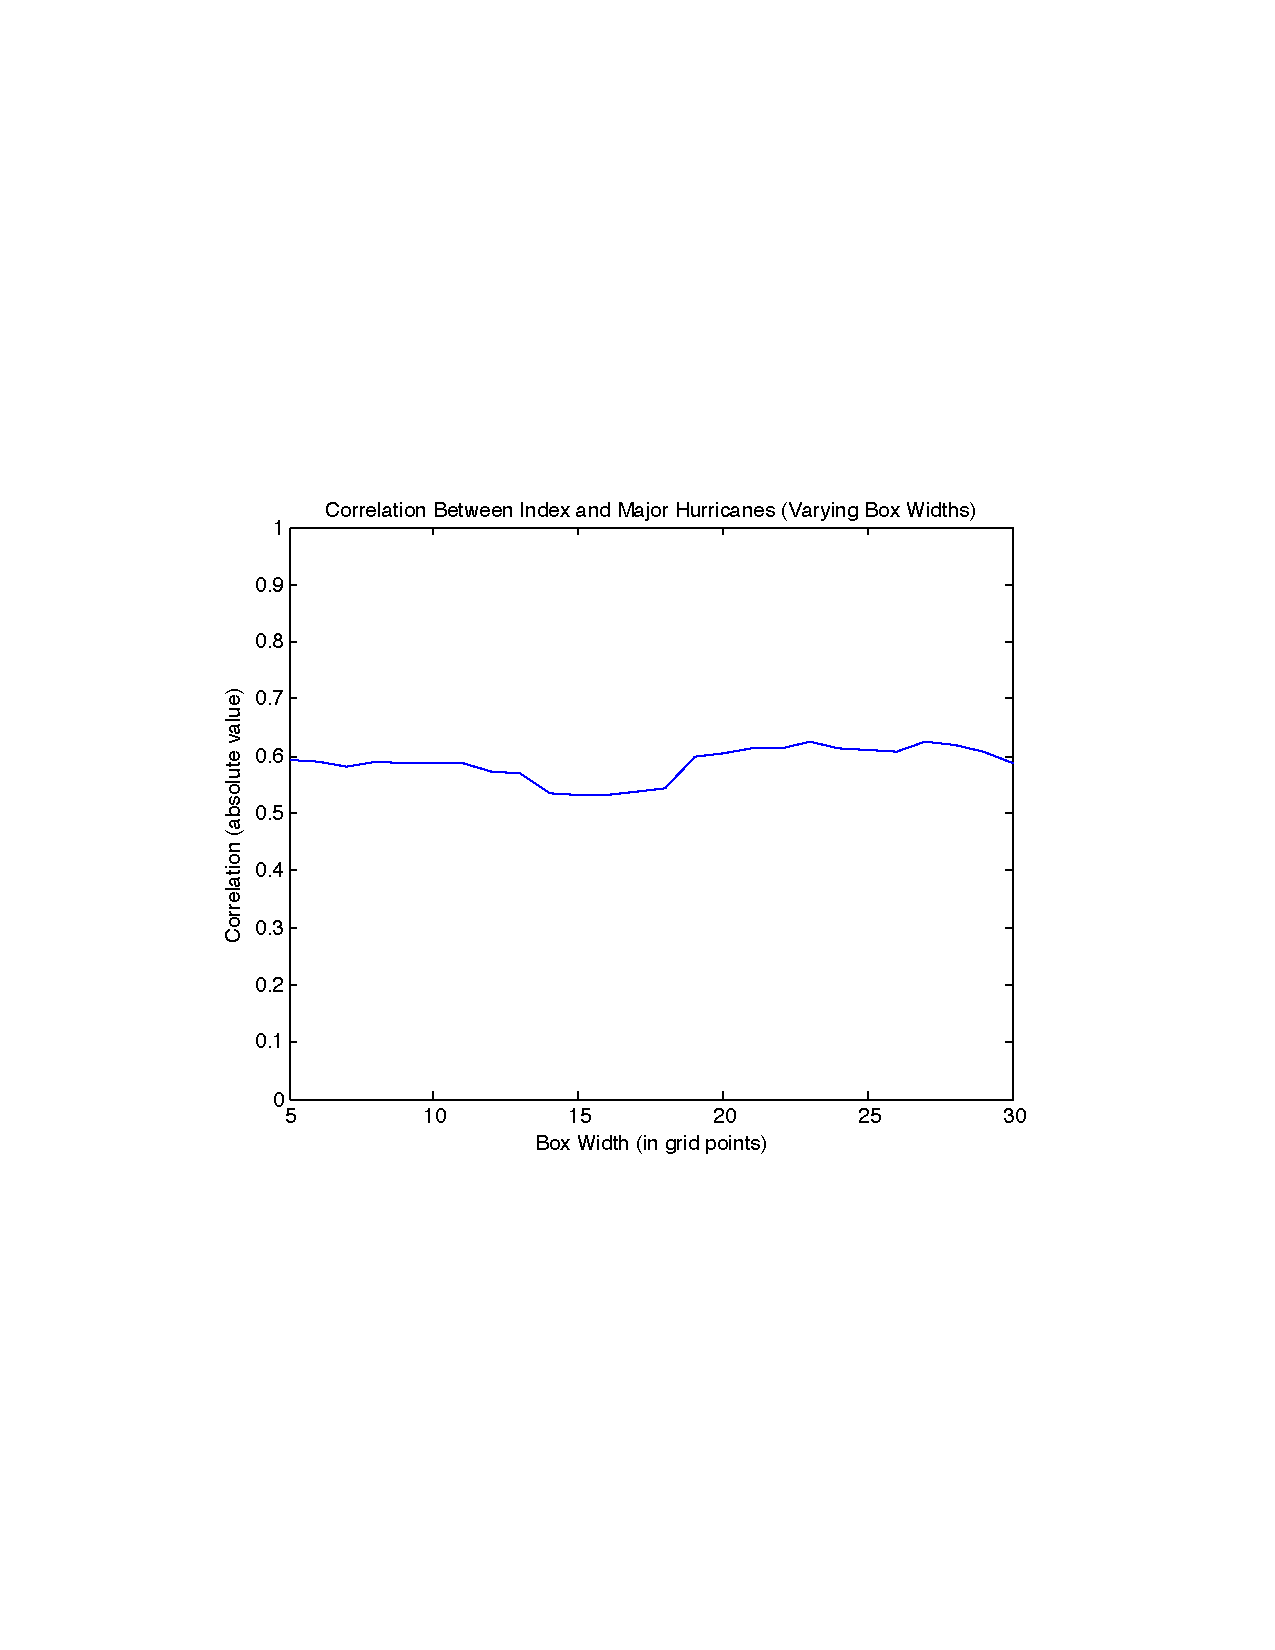
\includegraphics[width=\textwidth]{figures/sensitivityResults/boxSize/Major_Hurricanes_Index_Box_Size.pdf}
\caption{Corr Index vs. Major Hurricanes}
\label{fig:figure2}
\end{minipage}
\end{figure}

\begin{figure}[ht]
\begin{minipage}[b]{0.6\linewidth}
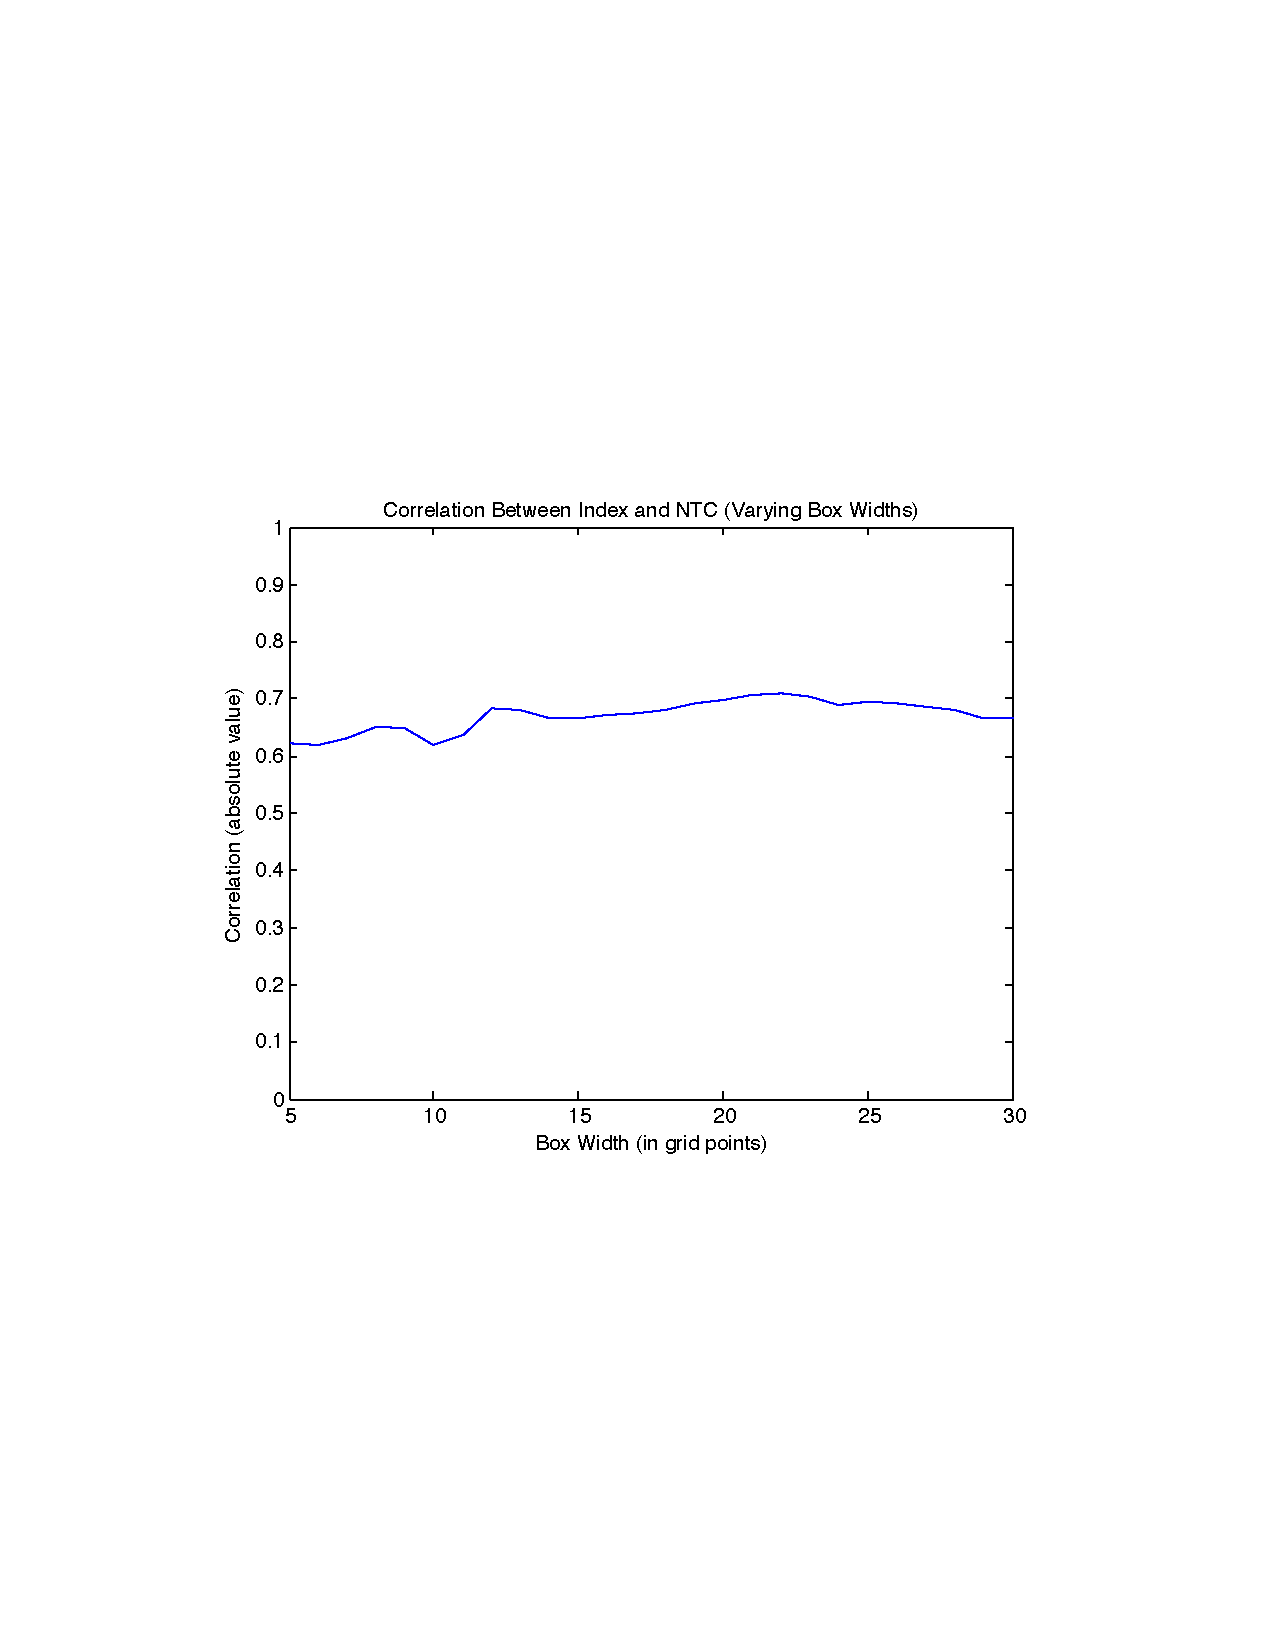
\includegraphics[width=\textwidth]{figures/sensitivityResults/boxSize/NTC_Index_Box_Size.pdf}
\caption{Corr Index vs. NTC}
\label{fig:figure3}
\end{minipage}
\hspace{0cm}
\begin{minipage}[b]{0.6\linewidth}
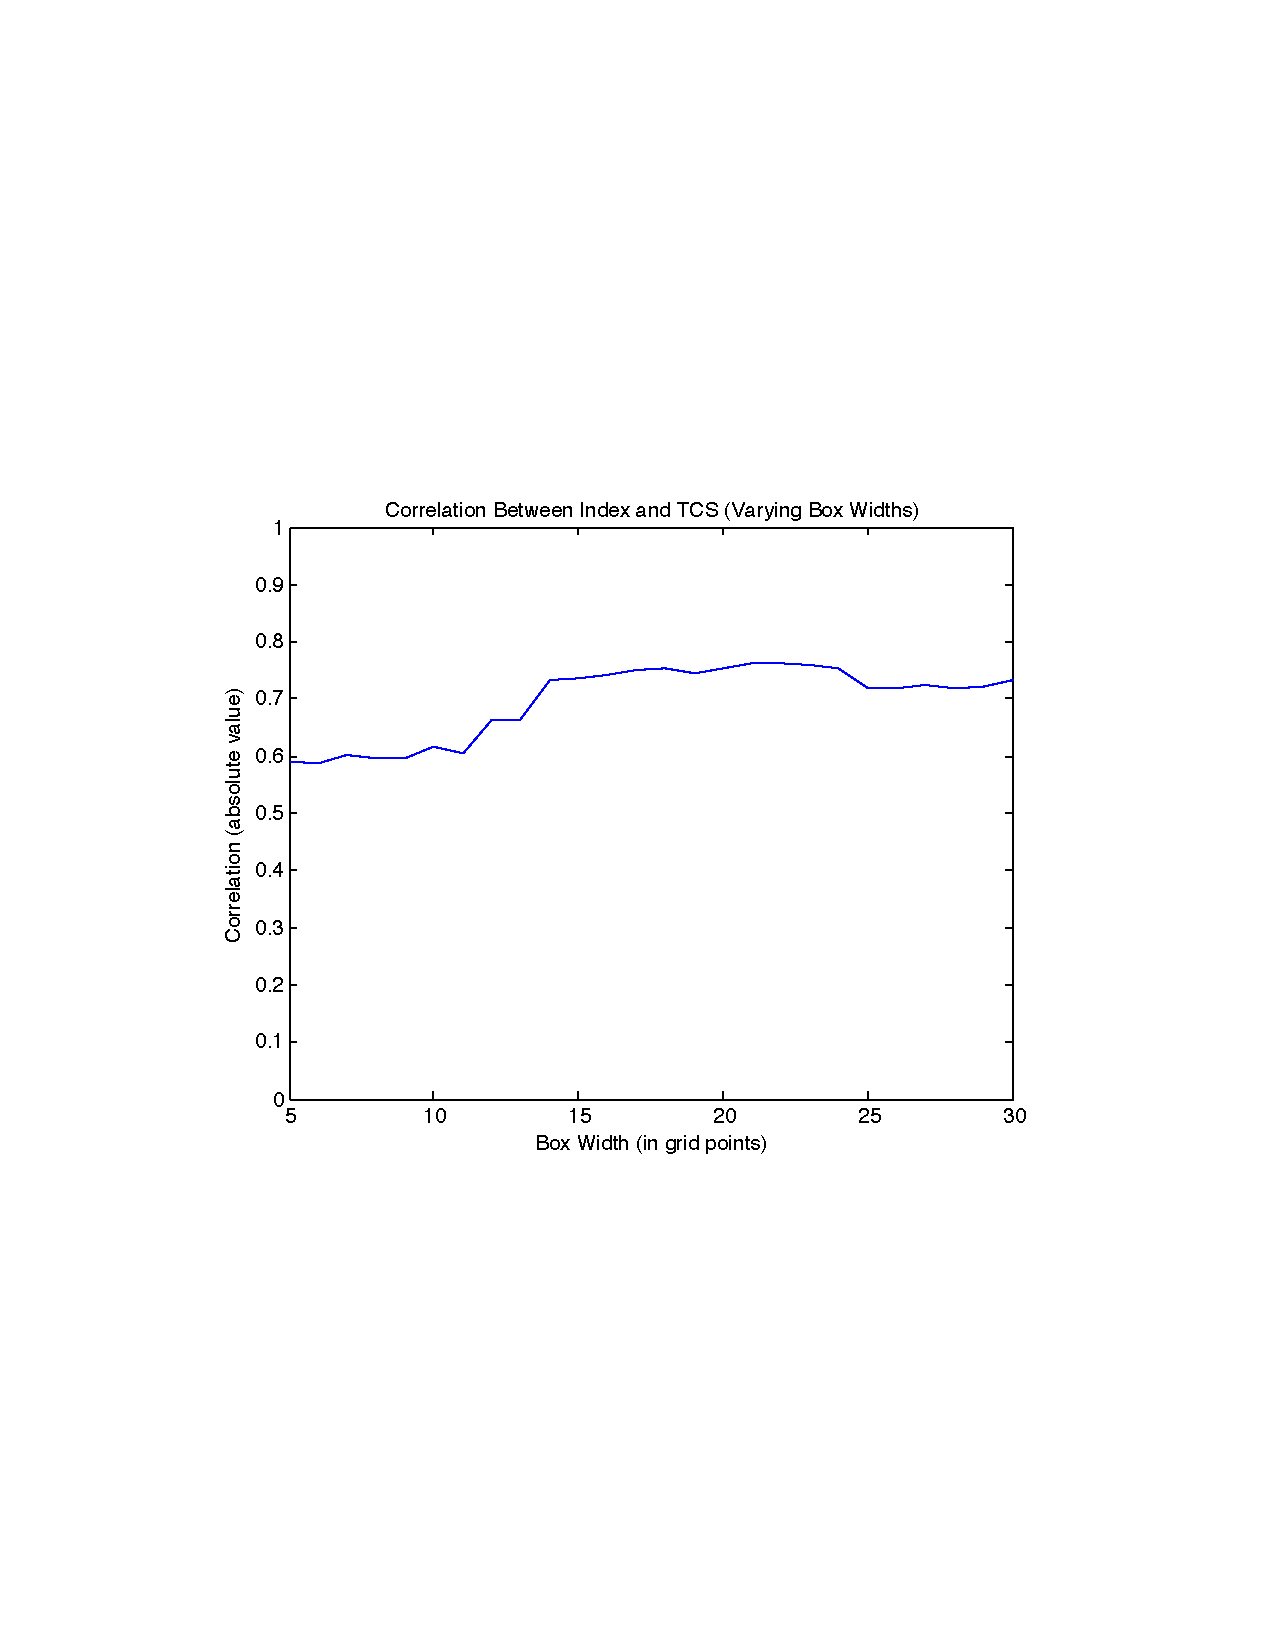
\includegraphics[width=\textwidth]{figures/sensitivityResults/boxSize/TCS_Index_Box_Size.pdf}
\caption{Corr Index vs. TCs}
\label{fig:figure4}
\end{minipage}
\end{figure}

\pagebreak
\subsection{Varying Month Ranges}

\begin{figure}[ht]
\begin{minipage}[b]{0.6\linewidth}
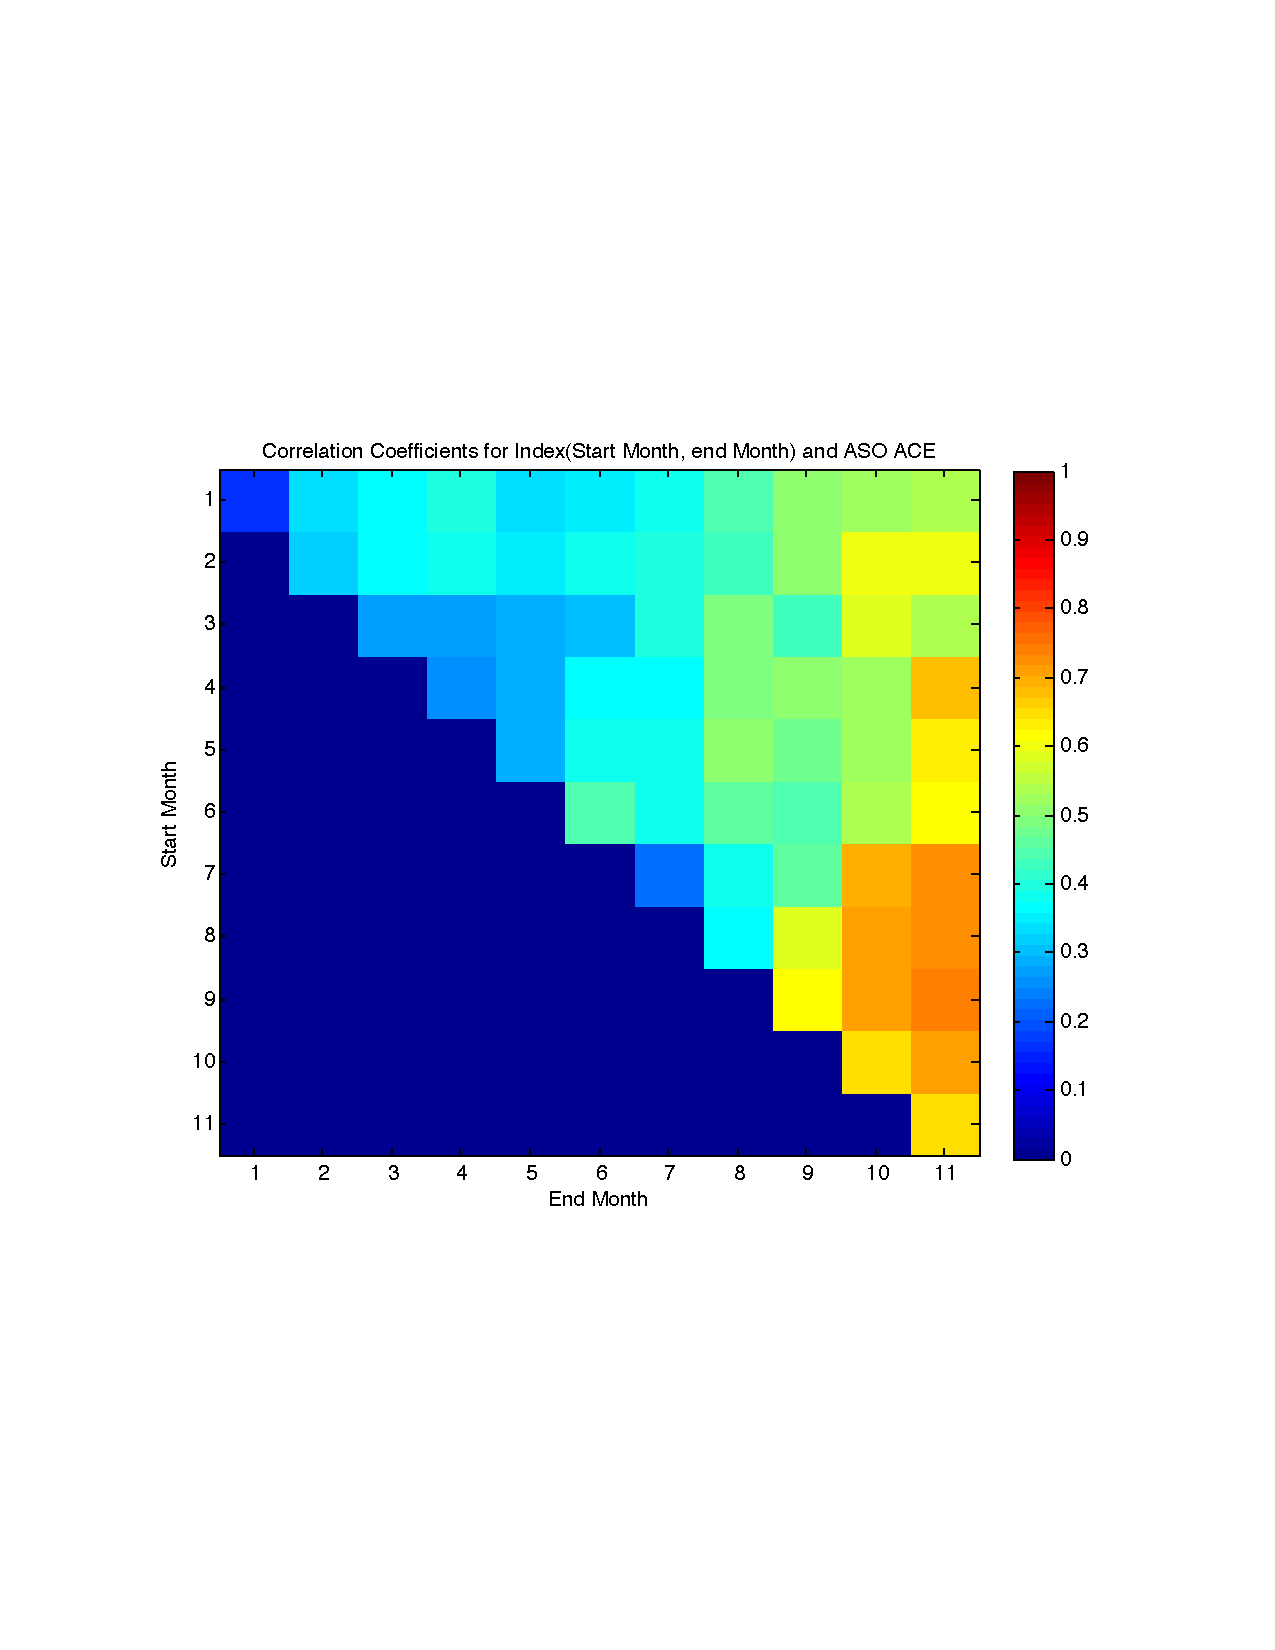
\includegraphics[width=\textwidth]{figures/sensitivityResults/monthRanges/index_corr_month_ranges_ace_month_range.pdf}
\caption{Corr Index vs. ACE}
\label{fig:figure5}
\end{minipage}
\hspace{0cm}
\begin{minipage}[b]{0.6\linewidth}
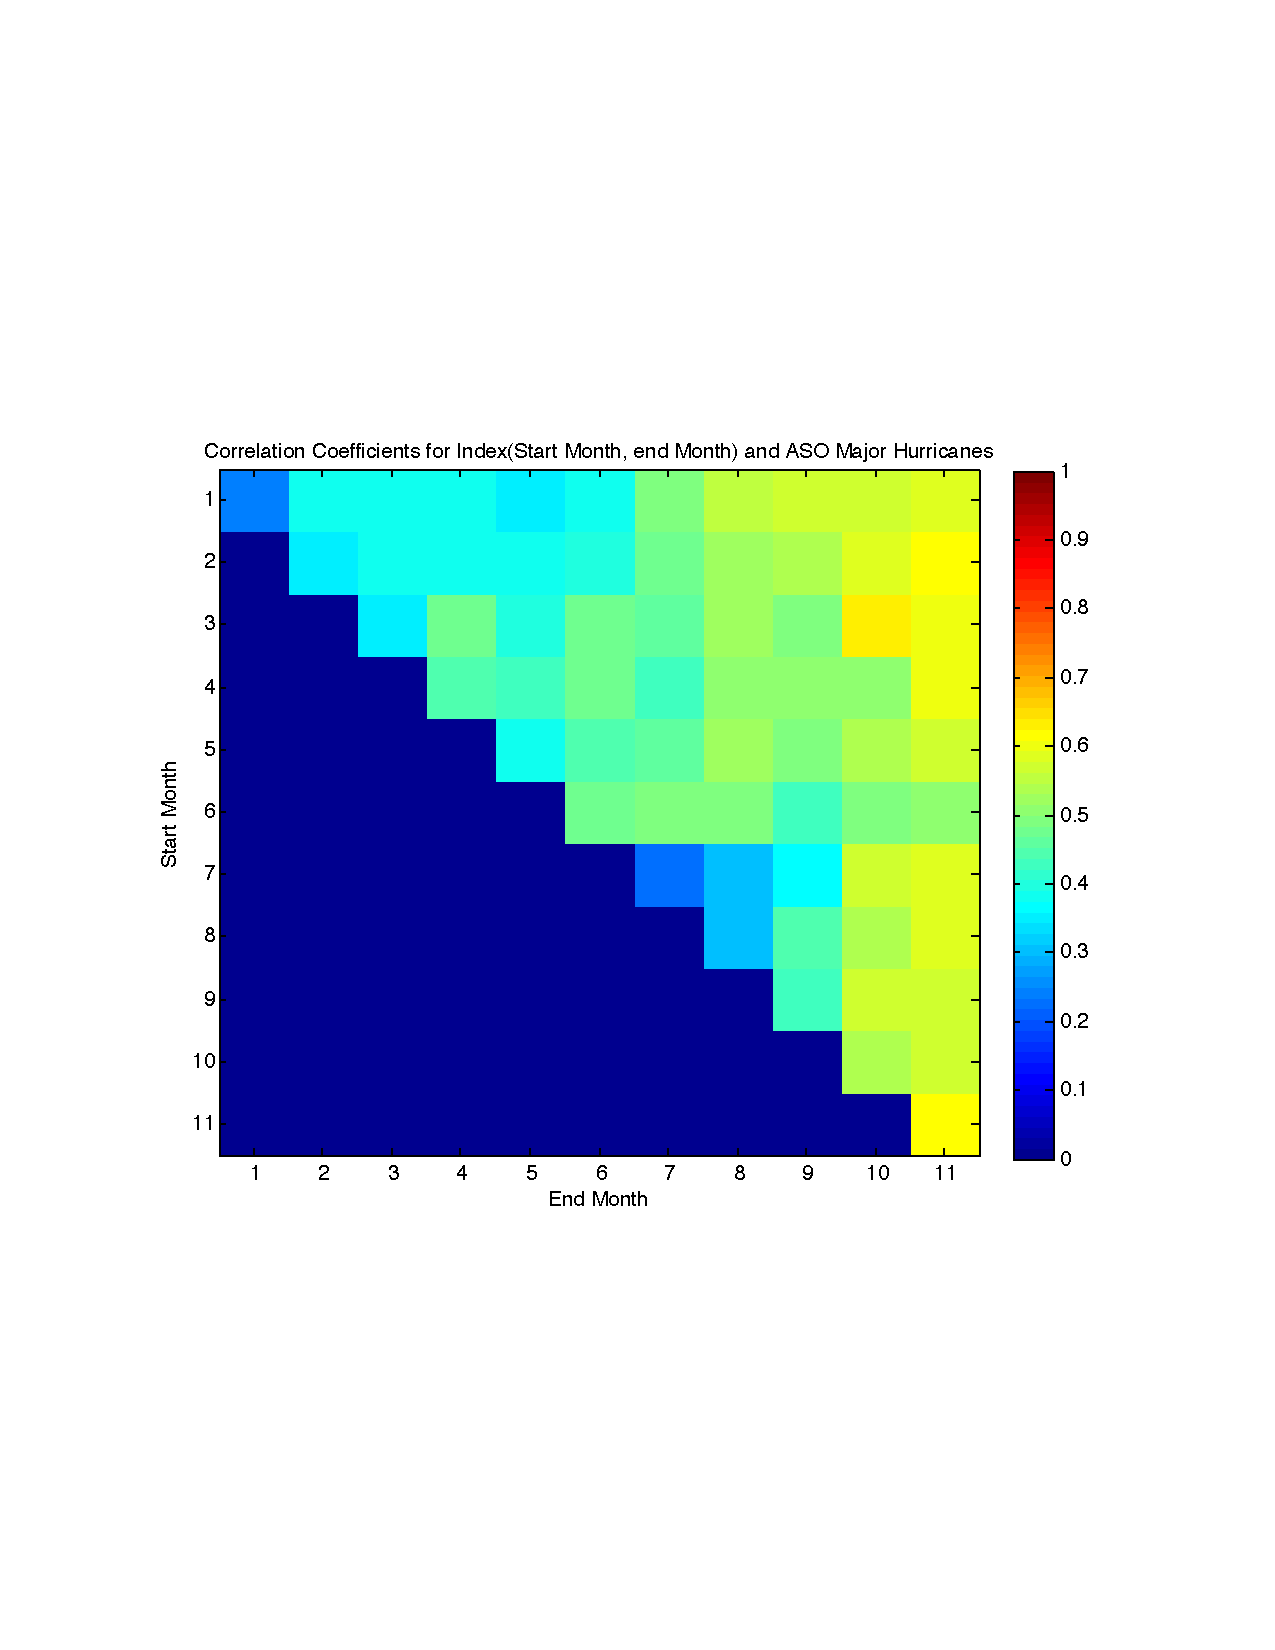
\includegraphics[width=\textwidth]{figures/sensitivityResults/monthRanges/index_corr_month_ranges_hurr_month_range.pdf}
\caption{Corr Index vs. Major Hurricanes}
\label{fig:figure6}
\end{minipage}
\end{figure}

\begin{figure}[ht]
\begin{minipage}[b]{0.6\linewidth}
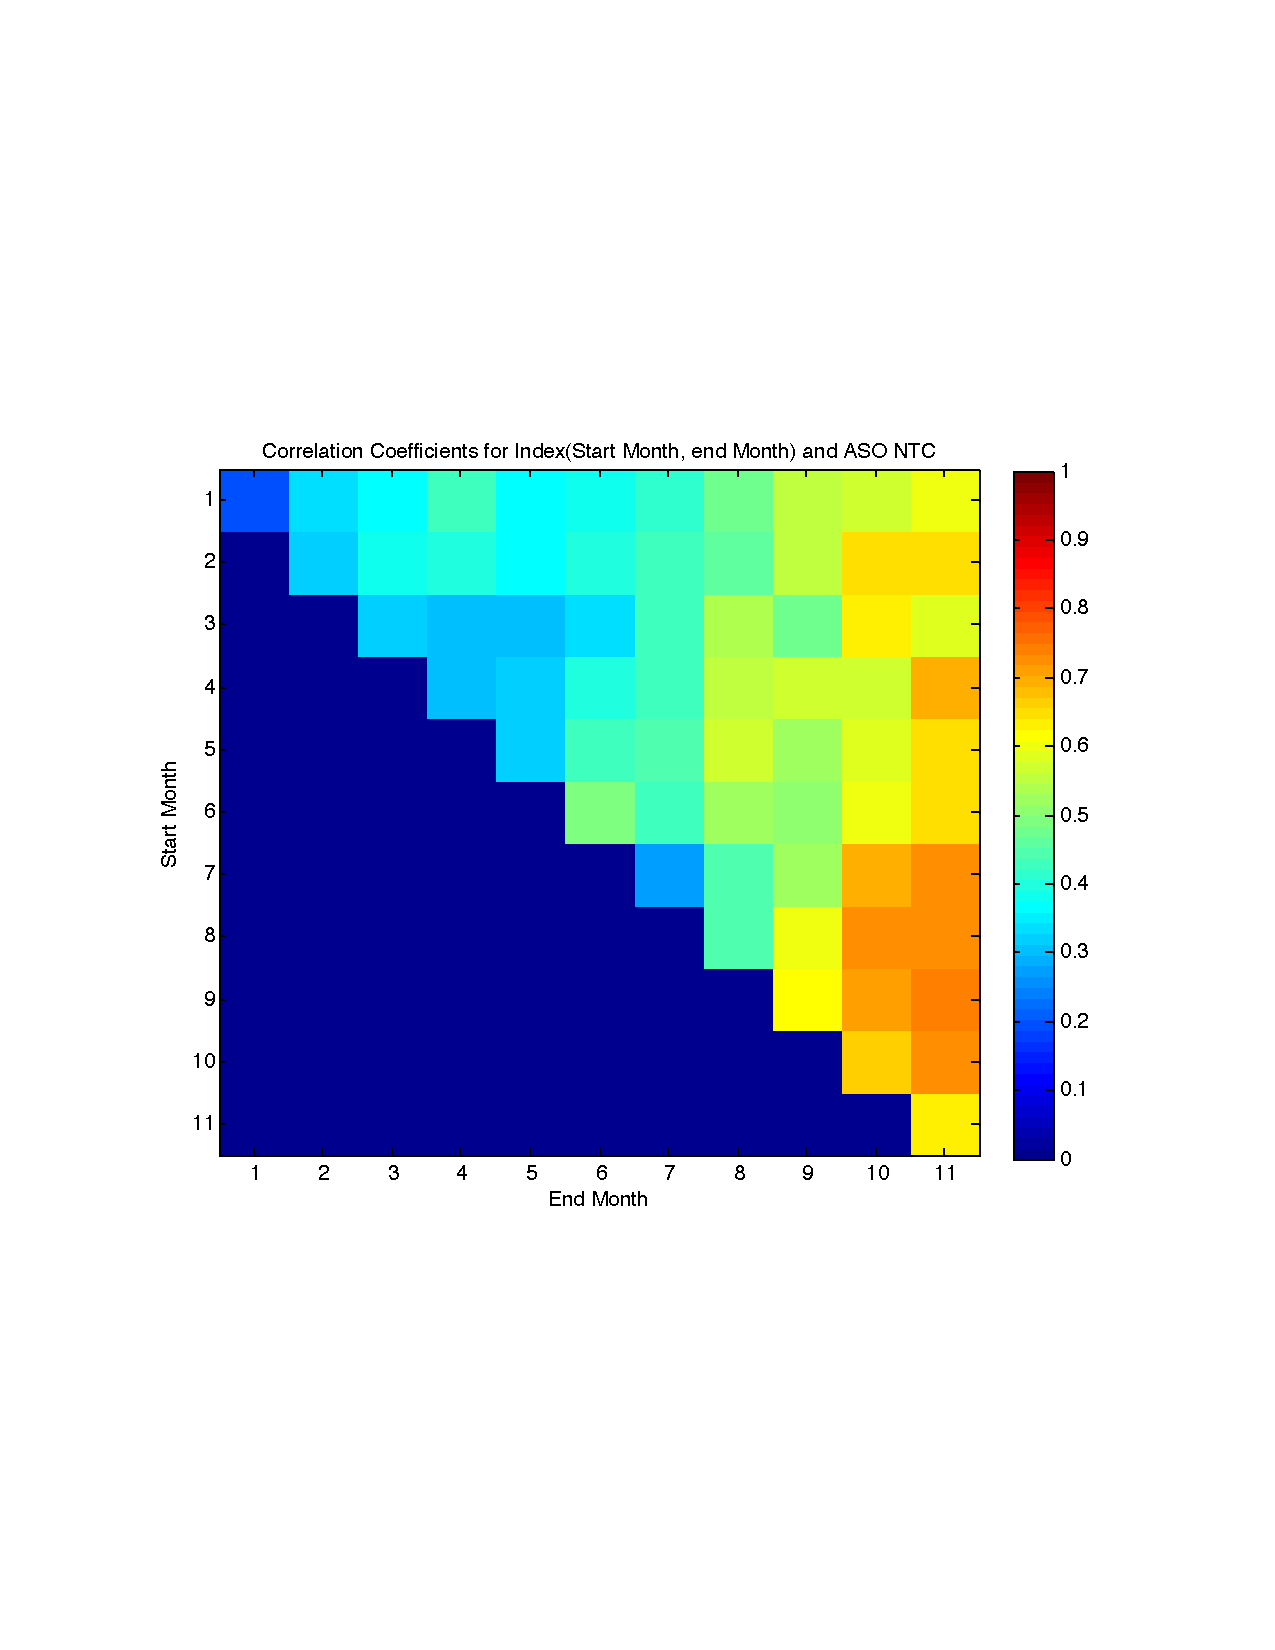
\includegraphics[width=\textwidth]{figures/sensitivityResults/monthRanges/index_corr_month_ranges_ntc_month_range.pdf}
\caption{Corr Index vs. NTC}
\label{fig:figure7}
\end{minipage}
\hspace{0cm}
\begin{minipage}[b]{0.6\linewidth}
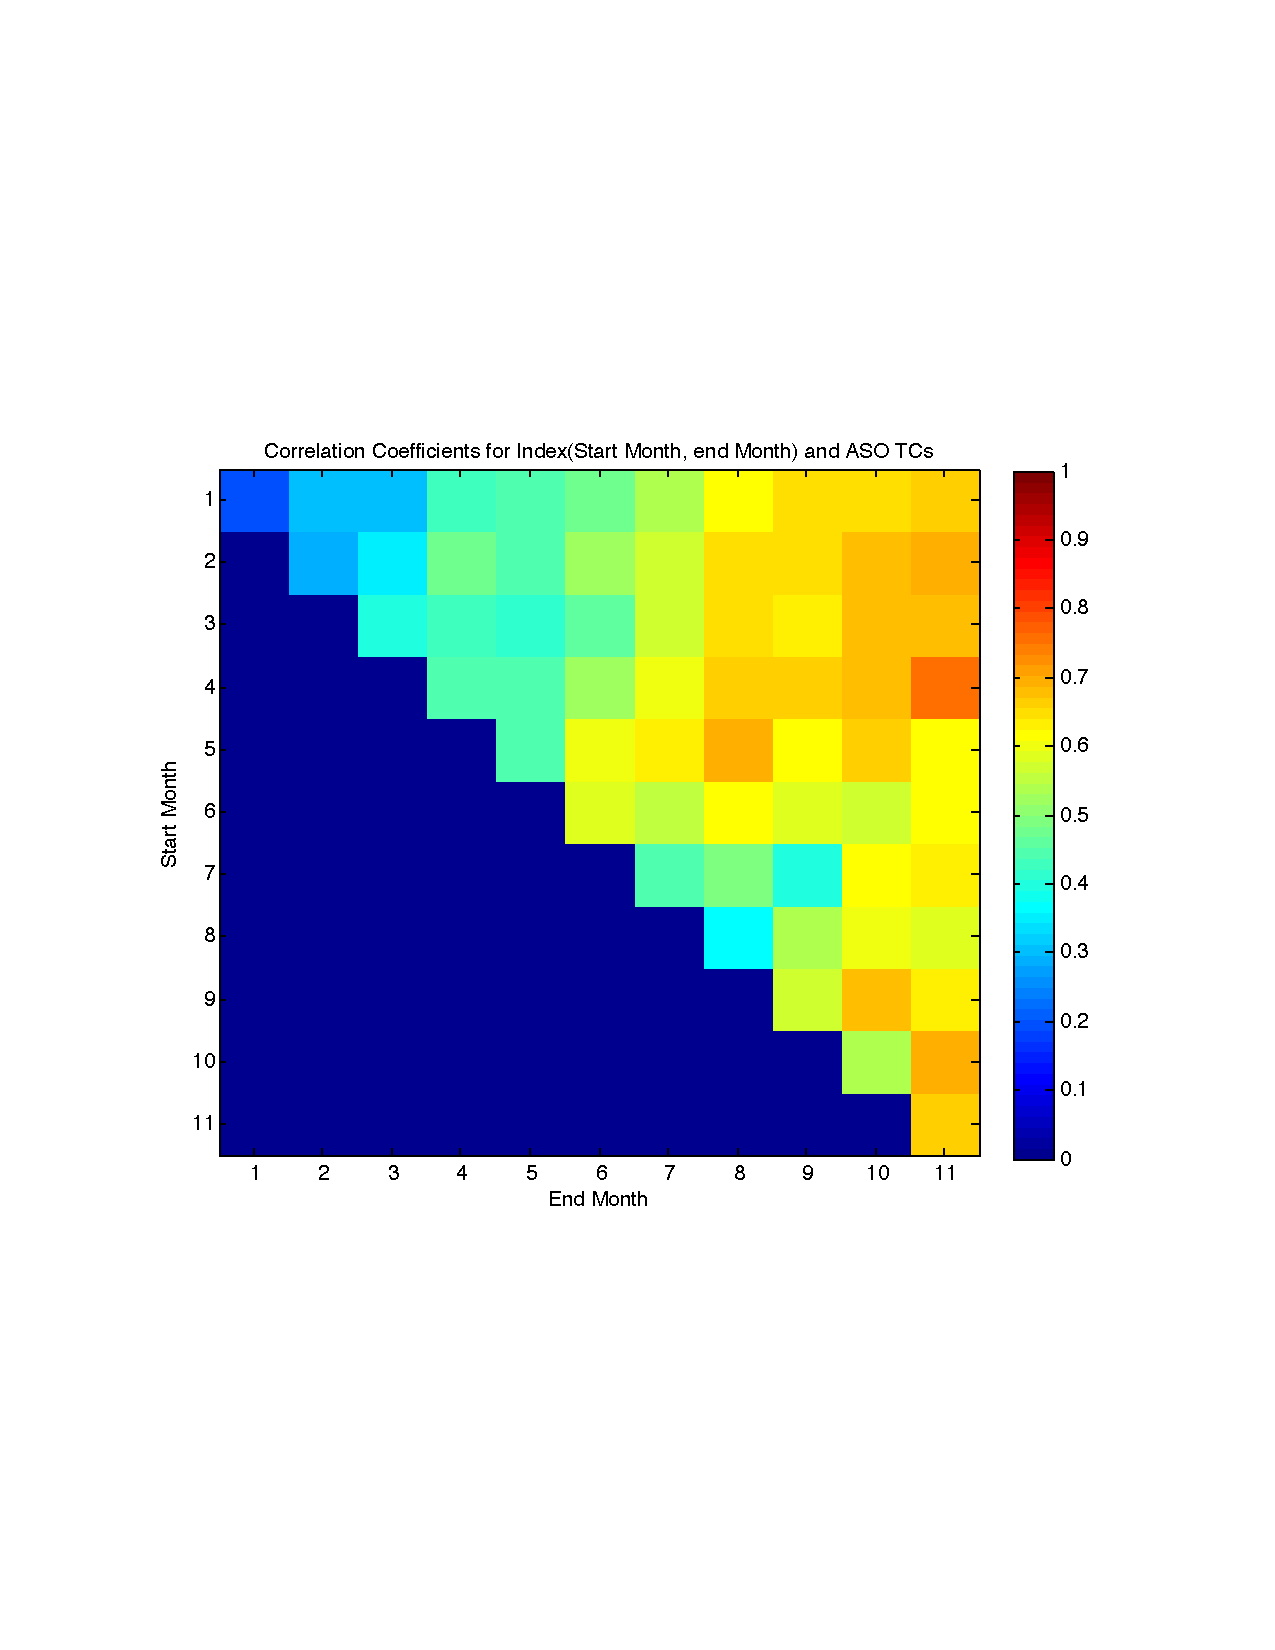
\includegraphics[width=\textwidth]{figures/sensitivityResults/monthRanges/index_corr_month_ranges_tcs_month_range.pdf}
\caption{Corr Index vs. TCs}
\label{fig:figure8}
\end{minipage}
\end{figure}

\pagebreak
\subsection{Varying Search Space (North and South Hemispheres)}
\begin{figure}[ht]
\begin{minipage}[b]{0.6\linewidth}
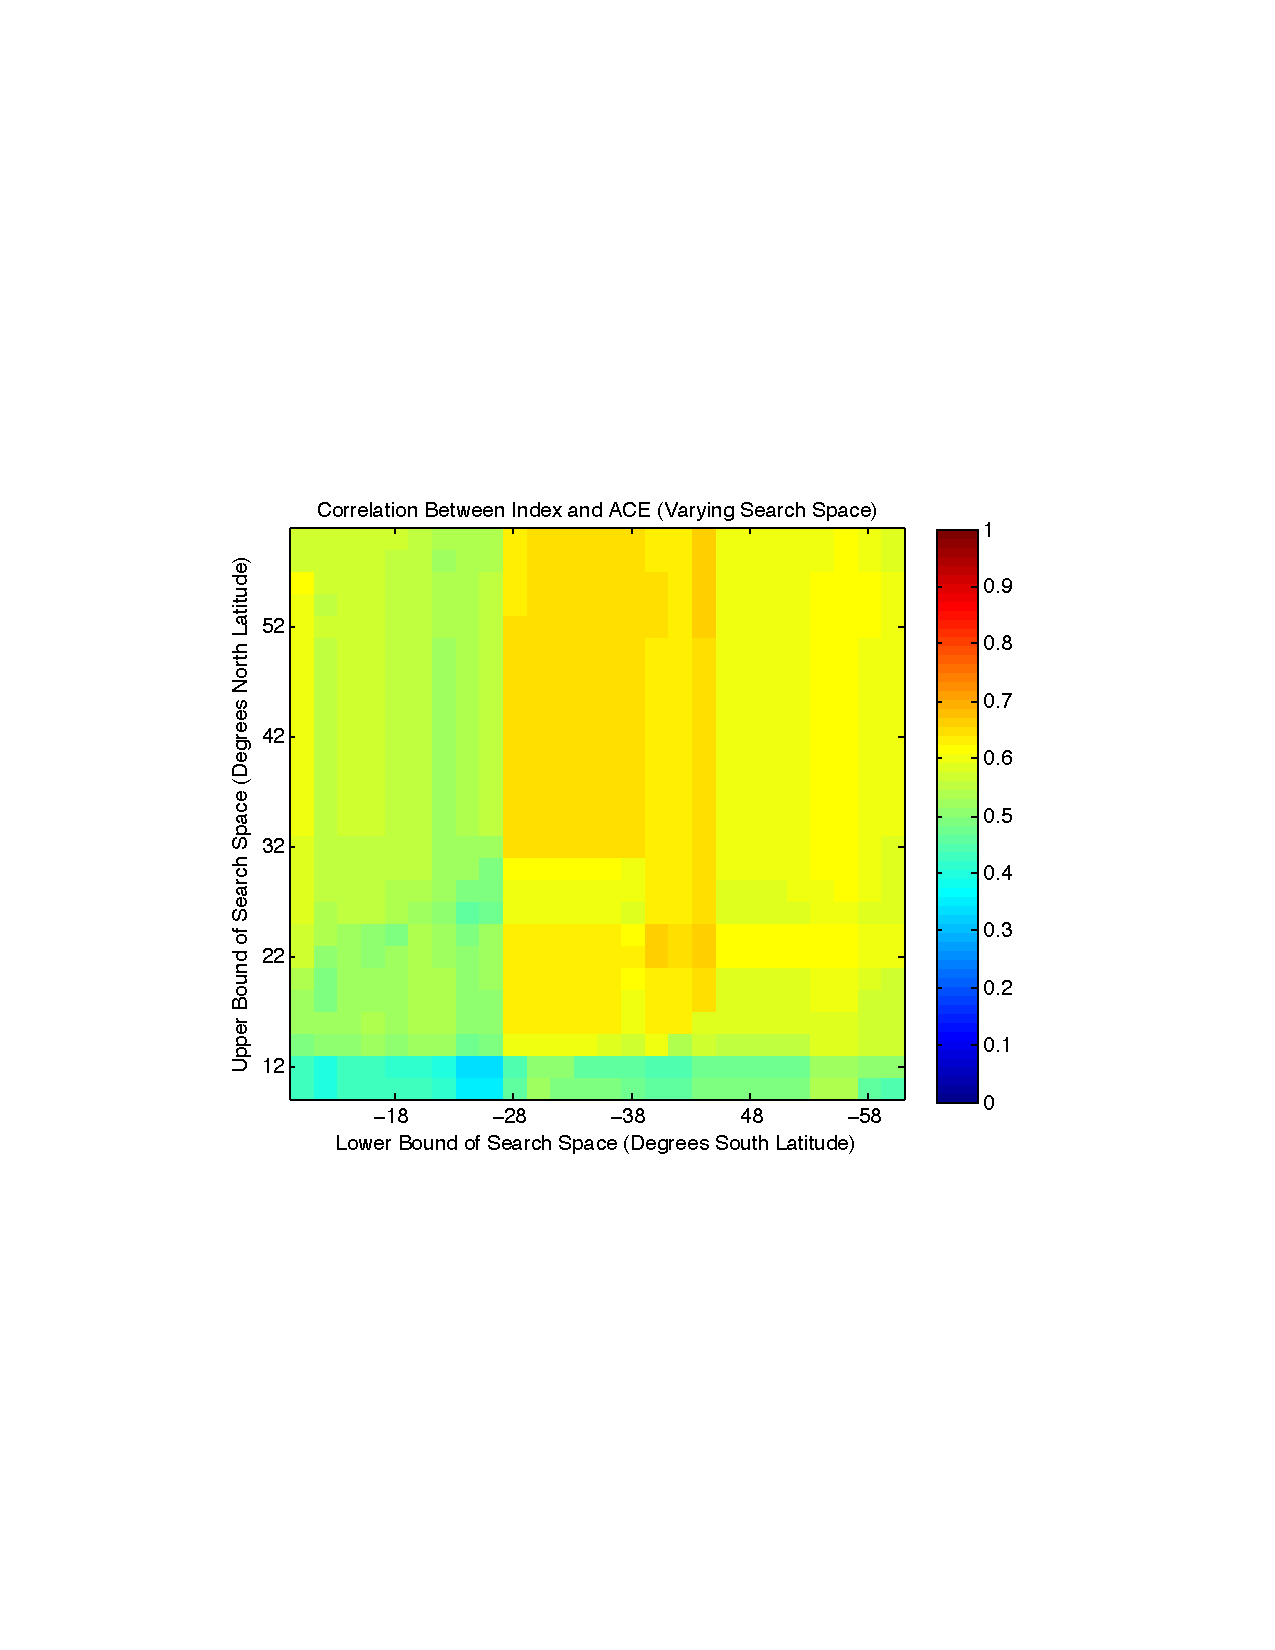
\includegraphics[width=\textwidth]{figures/sensitivityResults/northSouthHem/ACE_Index_North_South.pdf}
\caption{Corr Index vs. ACE}
\label{fig:figure9}
\end{minipage}
\hspace{0cm}
\begin{minipage}[b]{0.6\linewidth}
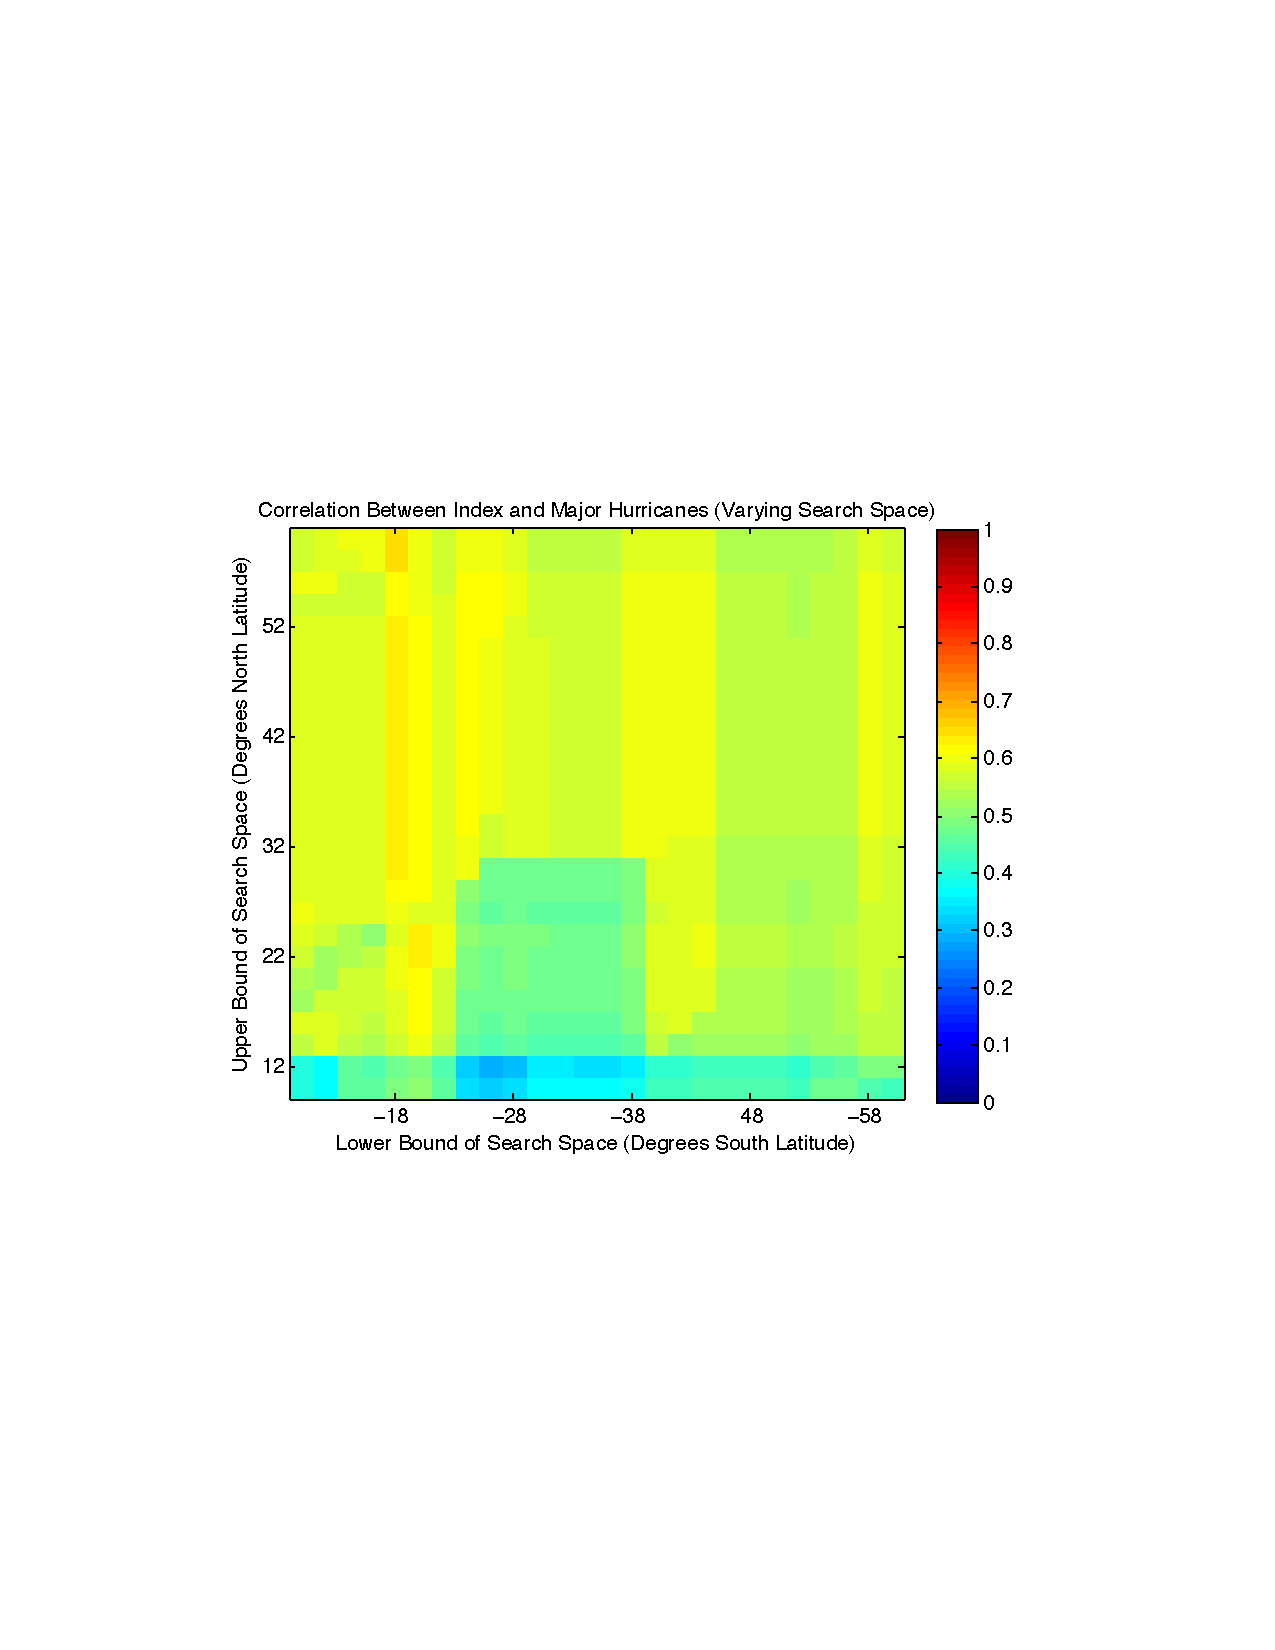
\includegraphics[width=\textwidth]{figures/sensitivityResults/northSouthHem/Major_Hurricanes_Index_North_South.pdf}
\caption{Corr Index vs. Major Hurricanes}
\label{fig:figure10}
\end{minipage}
\end{figure}

\begin{figure}[ht]
\begin{minipage}[b]{0.6\linewidth}
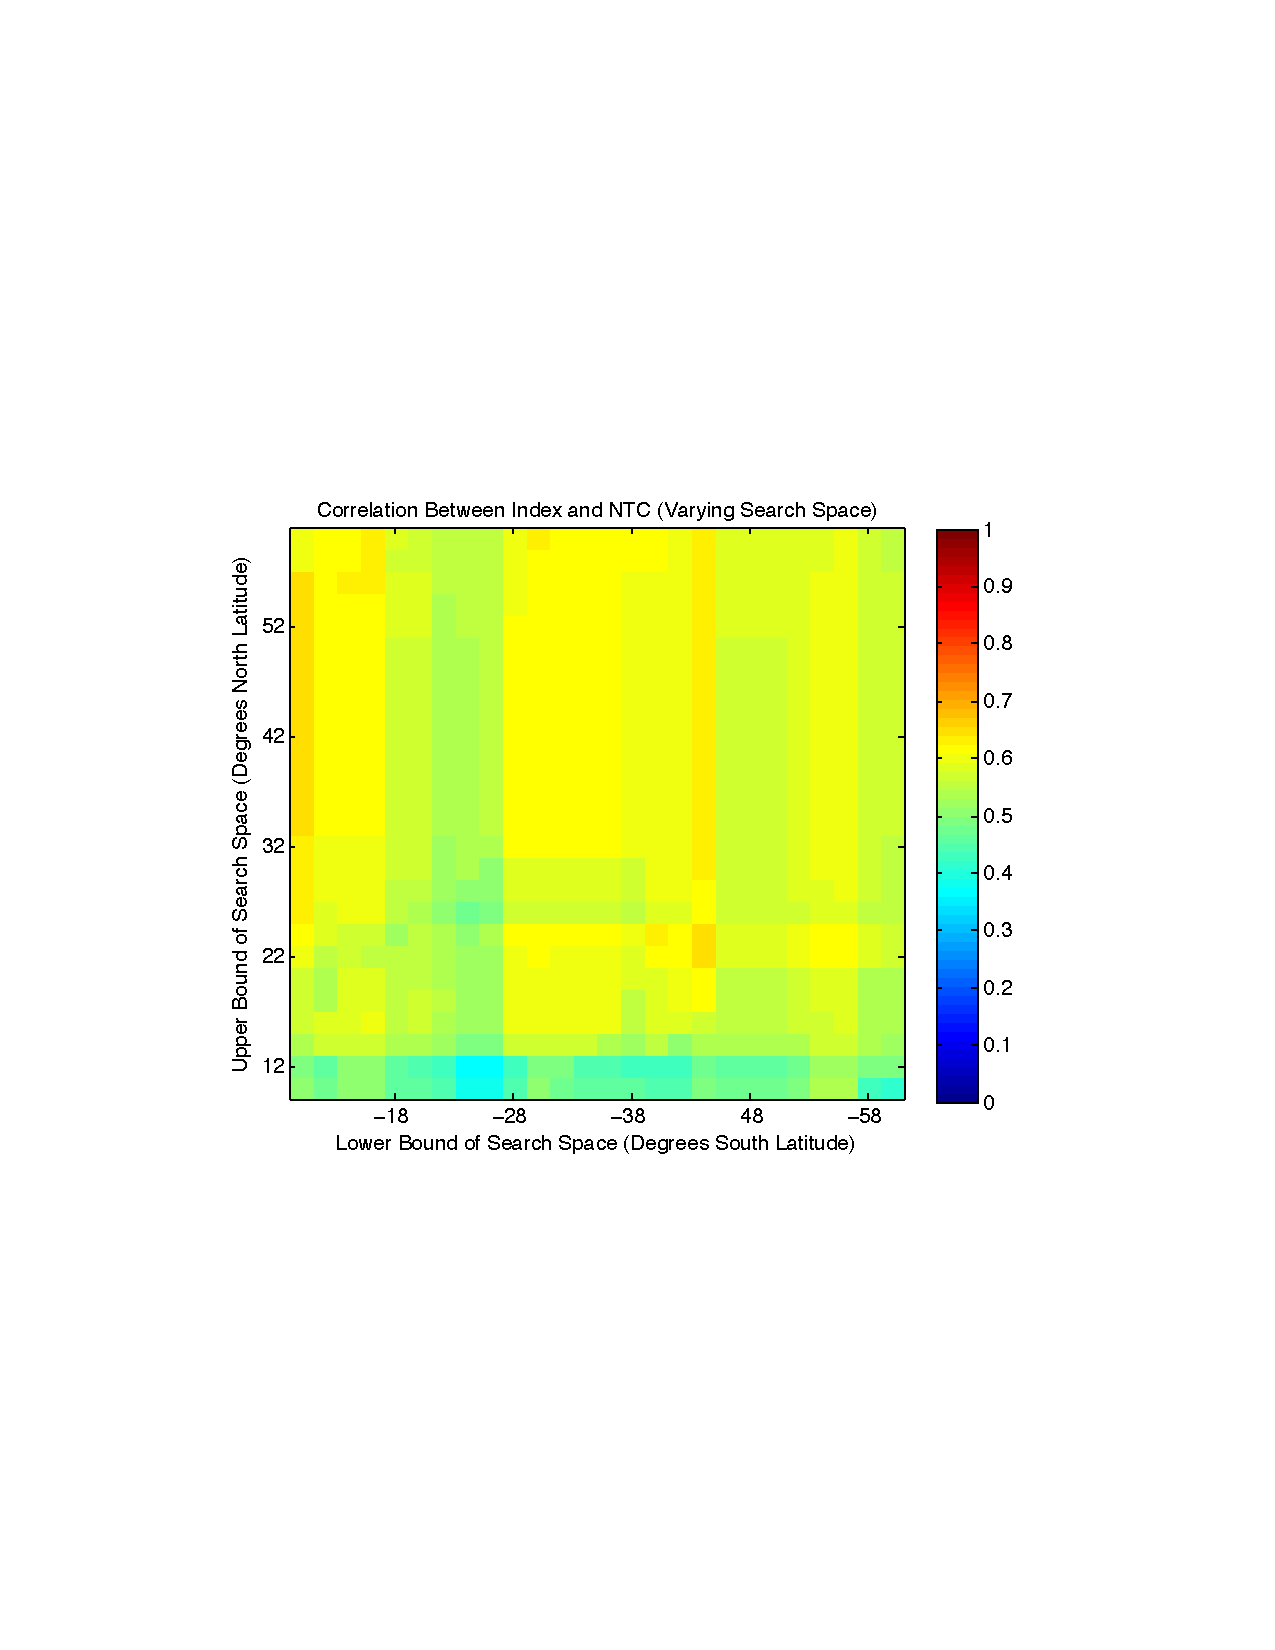
\includegraphics[width=\textwidth]{figures/sensitivityResults/northSouthHem/NTC_Index_North_South.pdf}
\caption{Corr Index vs. NTC}
\label{fig:figure11}
\end{minipage}
\hspace{0cm}
\begin{minipage}[b]{0.6\linewidth}
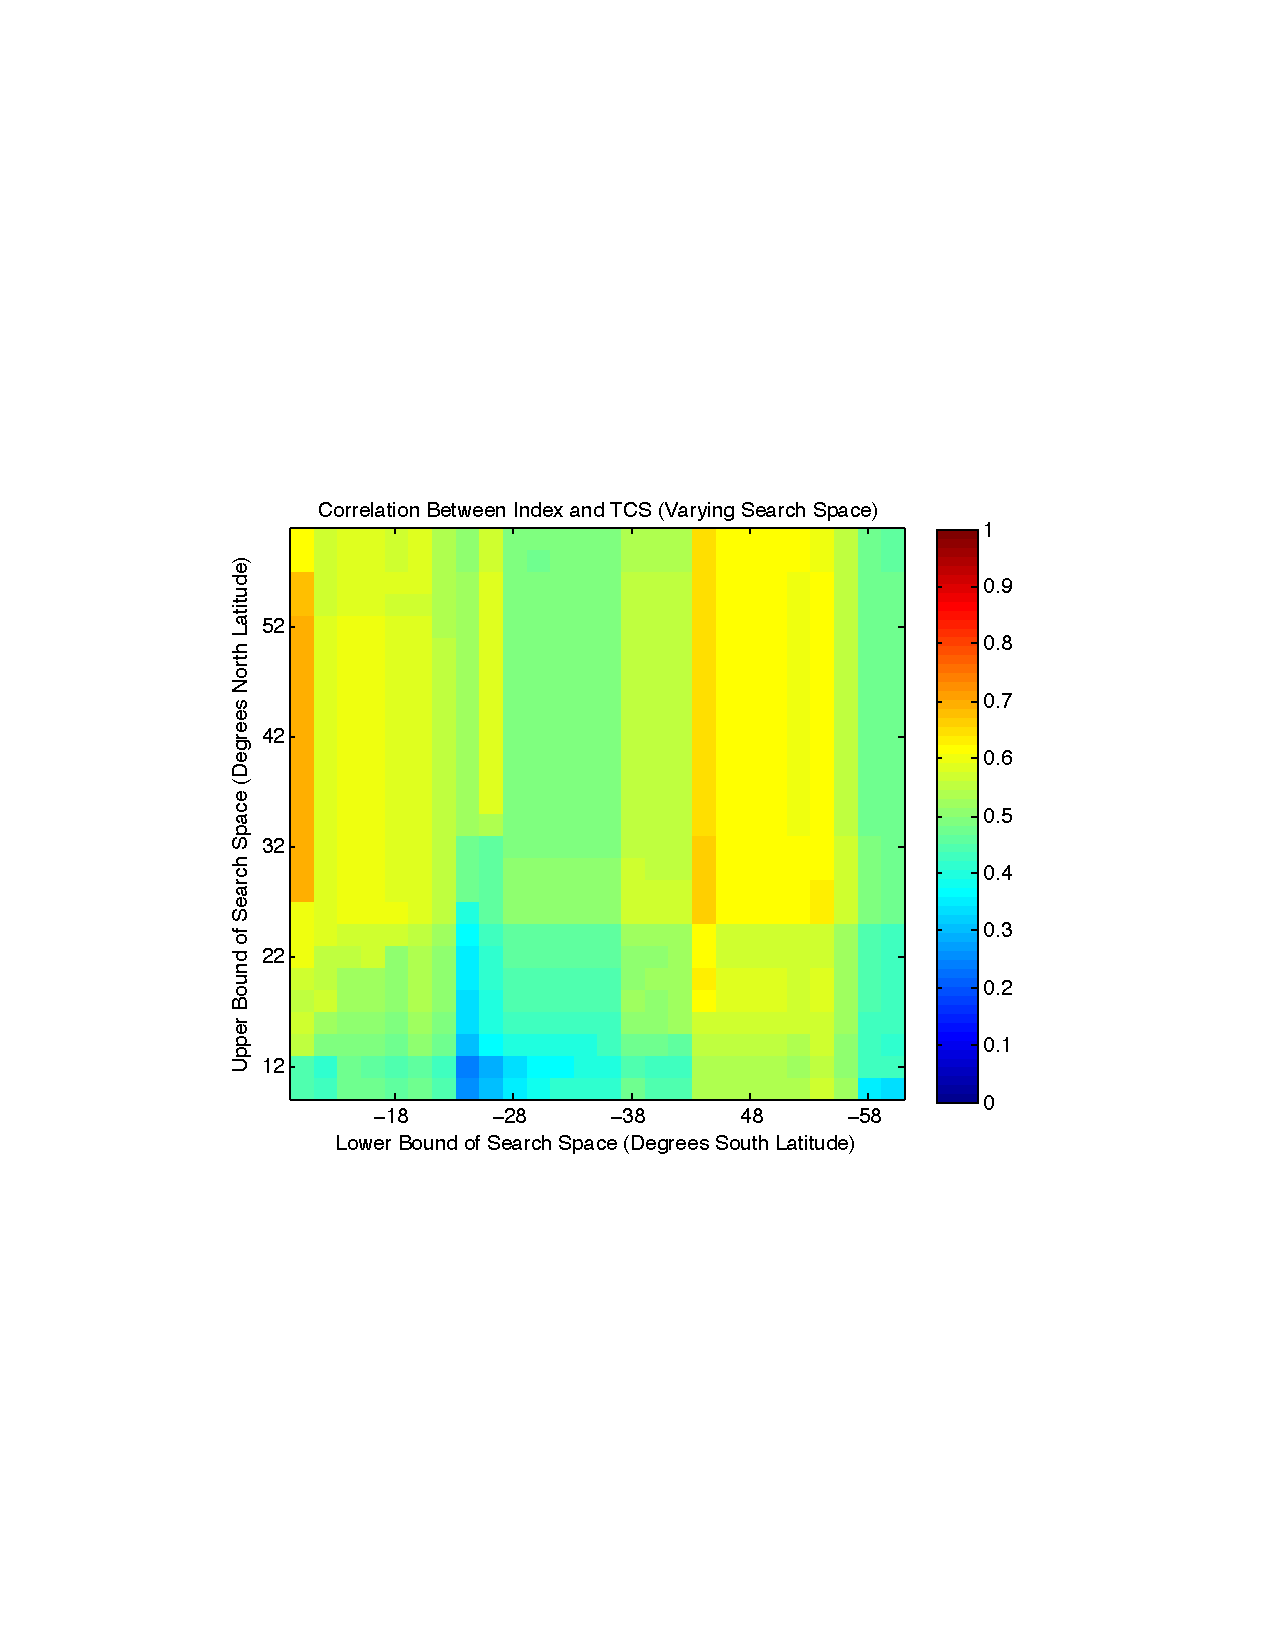
\includegraphics[width=\textwidth]{figures/sensitivityResults/northSouthHem/TCS_Index_North_South.pdf}
\caption{Corr Index vs. TCs}
\label{fig:figure12}
\end{minipage}
\end{figure}
\pagebreak

\subsection{Varying Search Space (North Hemisphere)}

\begin{figure}[ht]
\begin{minipage}[b]{0.6\linewidth}
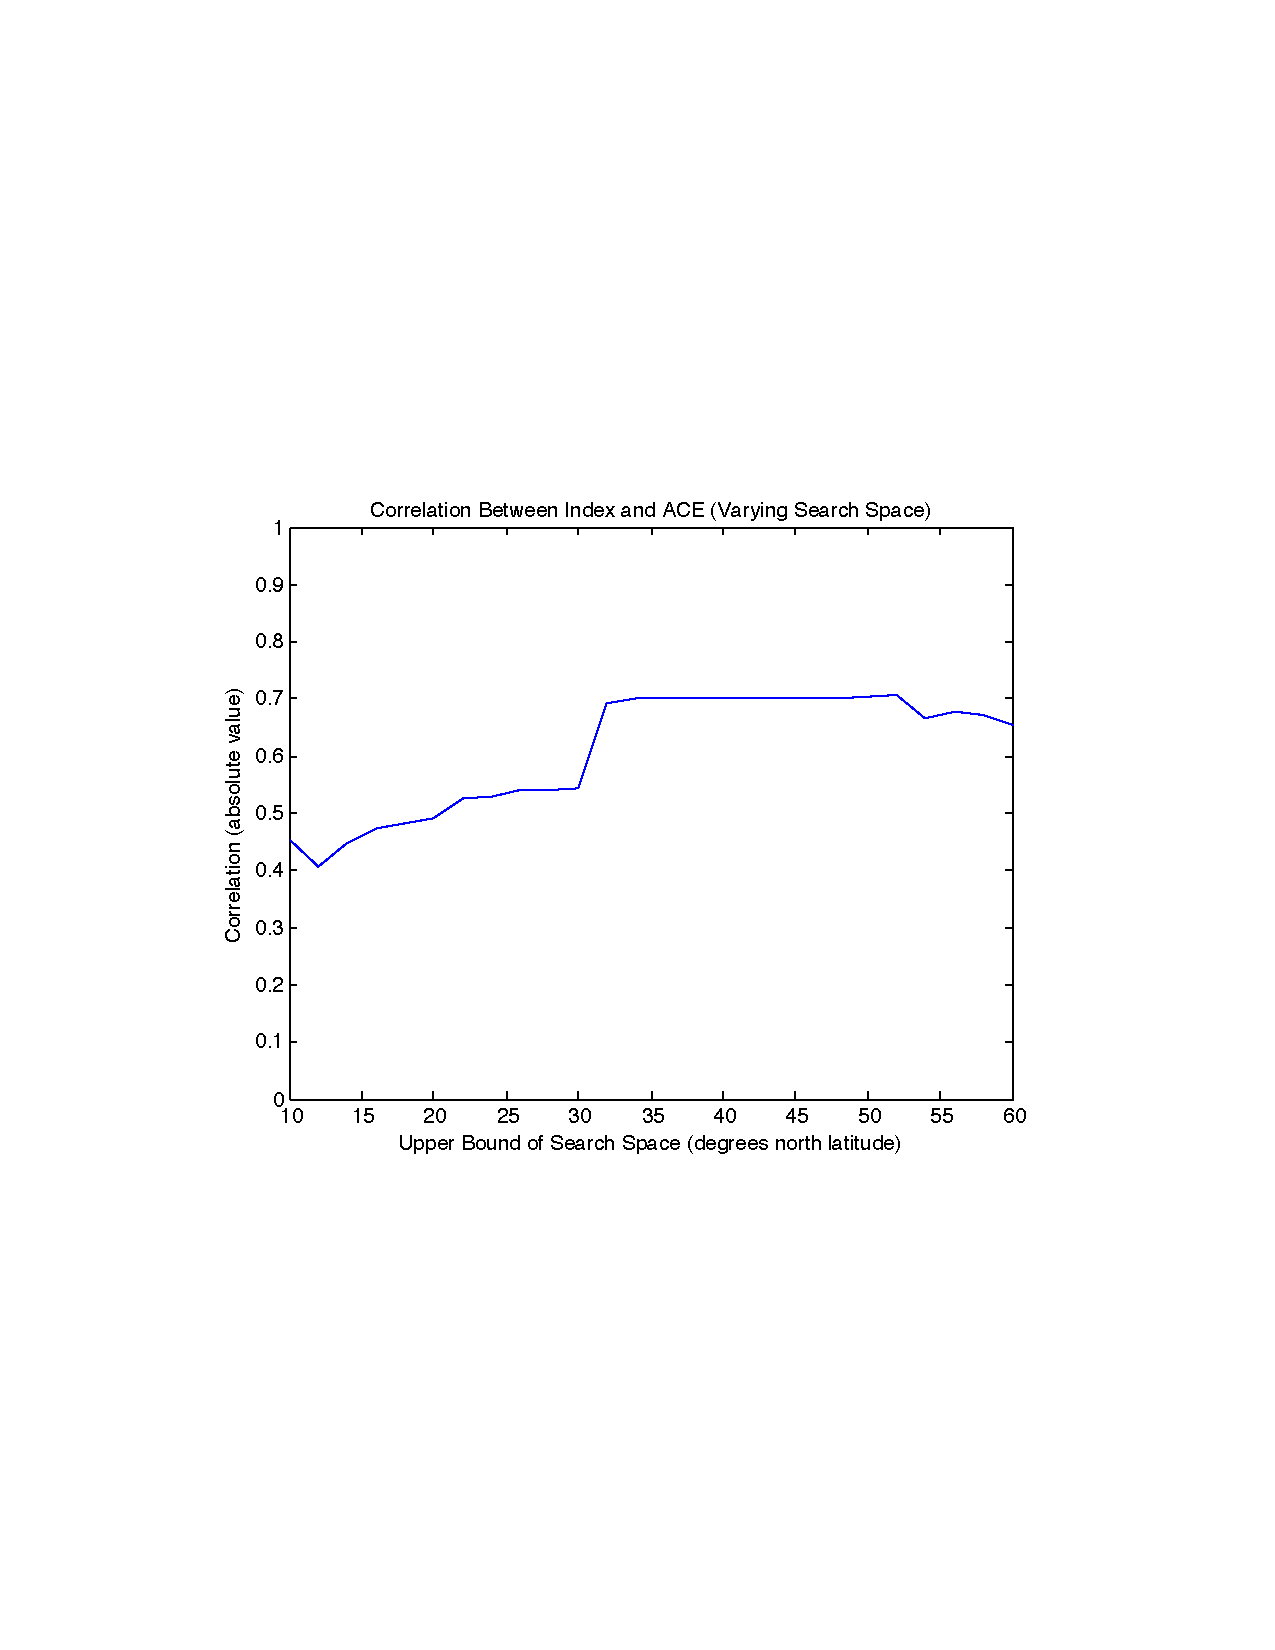
\includegraphics[width=\textwidth]{figures/sensitivityResults/northHem/ACE_Index_North.pdf}
\caption{Corr Index vs. ACE}
\label{fig:figure13}
\end{minipage}
\hspace{0cm}
\begin{minipage}[b]{0.6\linewidth}
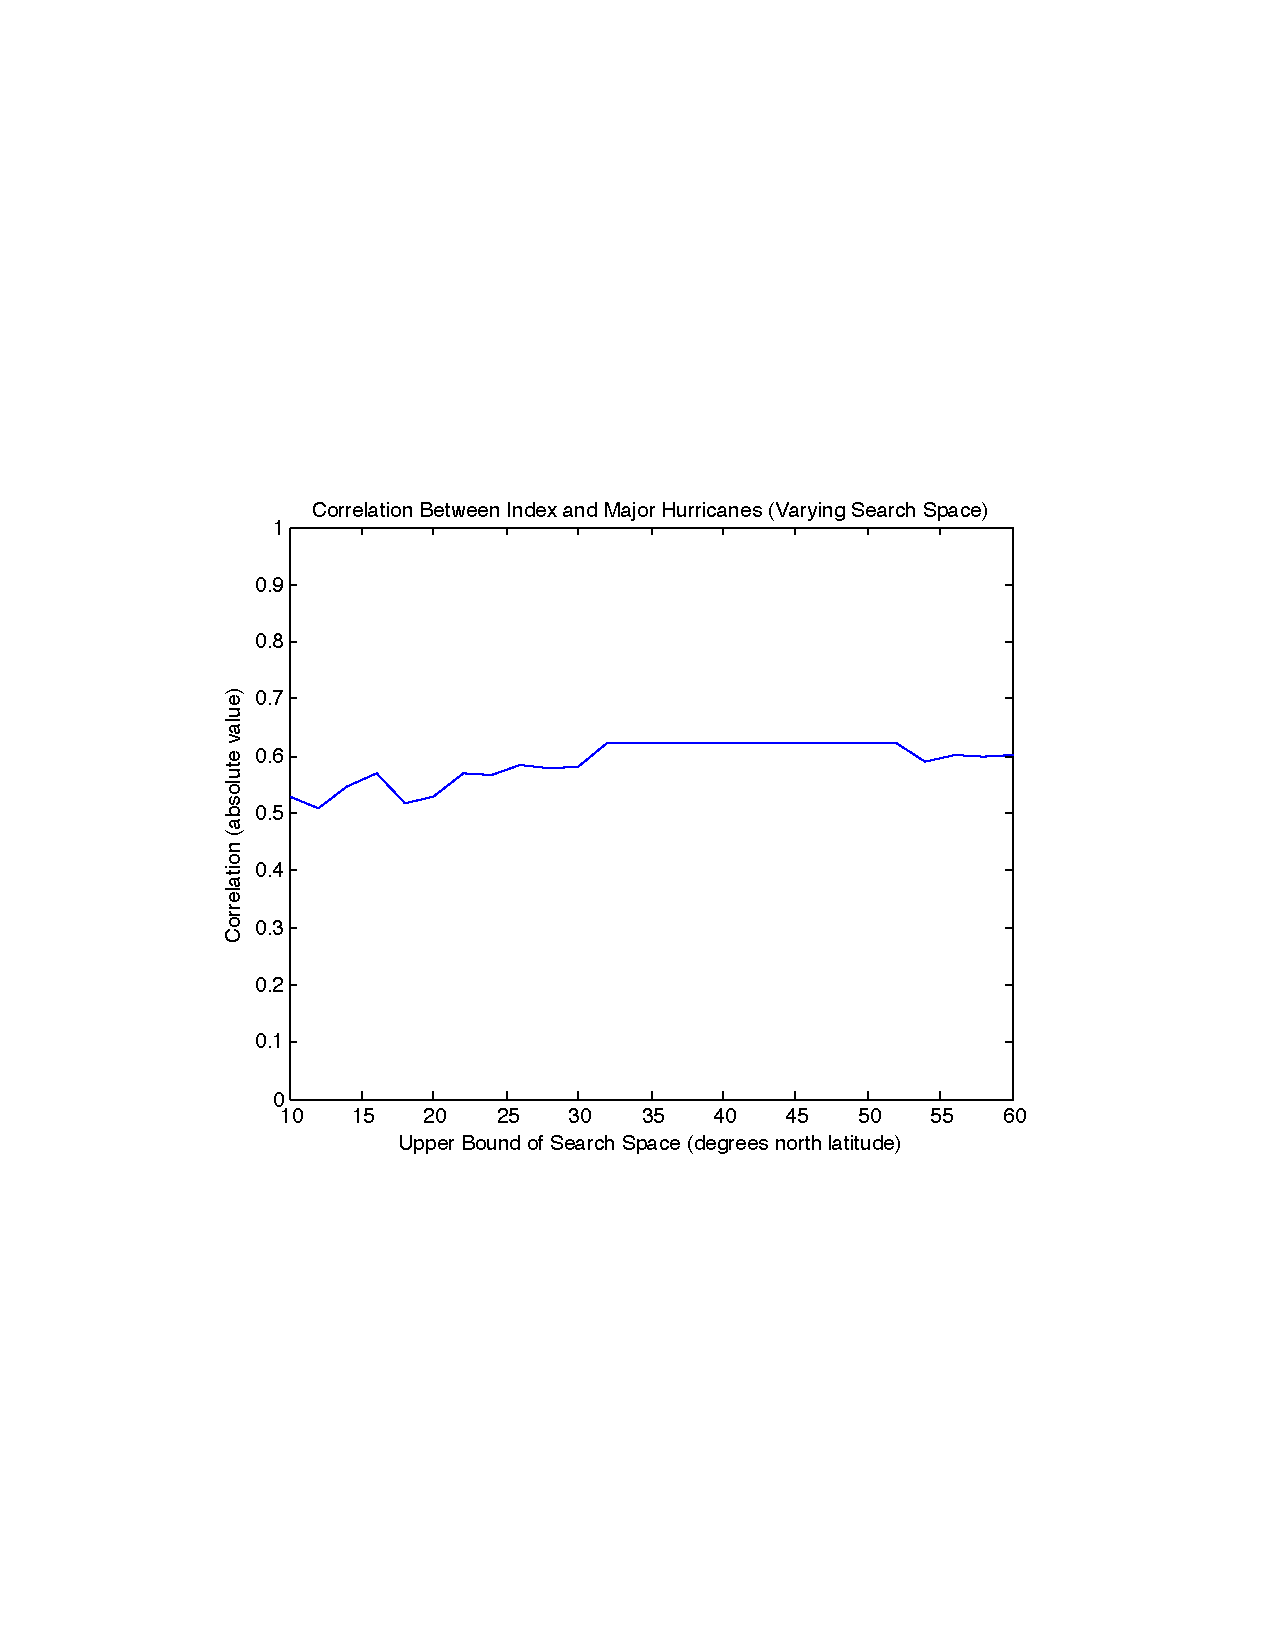
\includegraphics[width=\textwidth]{figures/sensitivityResults/northHem/Major_Hurricanes_Index_North.pdf}
\caption{Corr Index vs. Major Hurricanes}
\label{fig:figure14}
\end{minipage}
\end{figure}

\begin{figure}[ht]
\begin{minipage}[b]{0.6\linewidth}
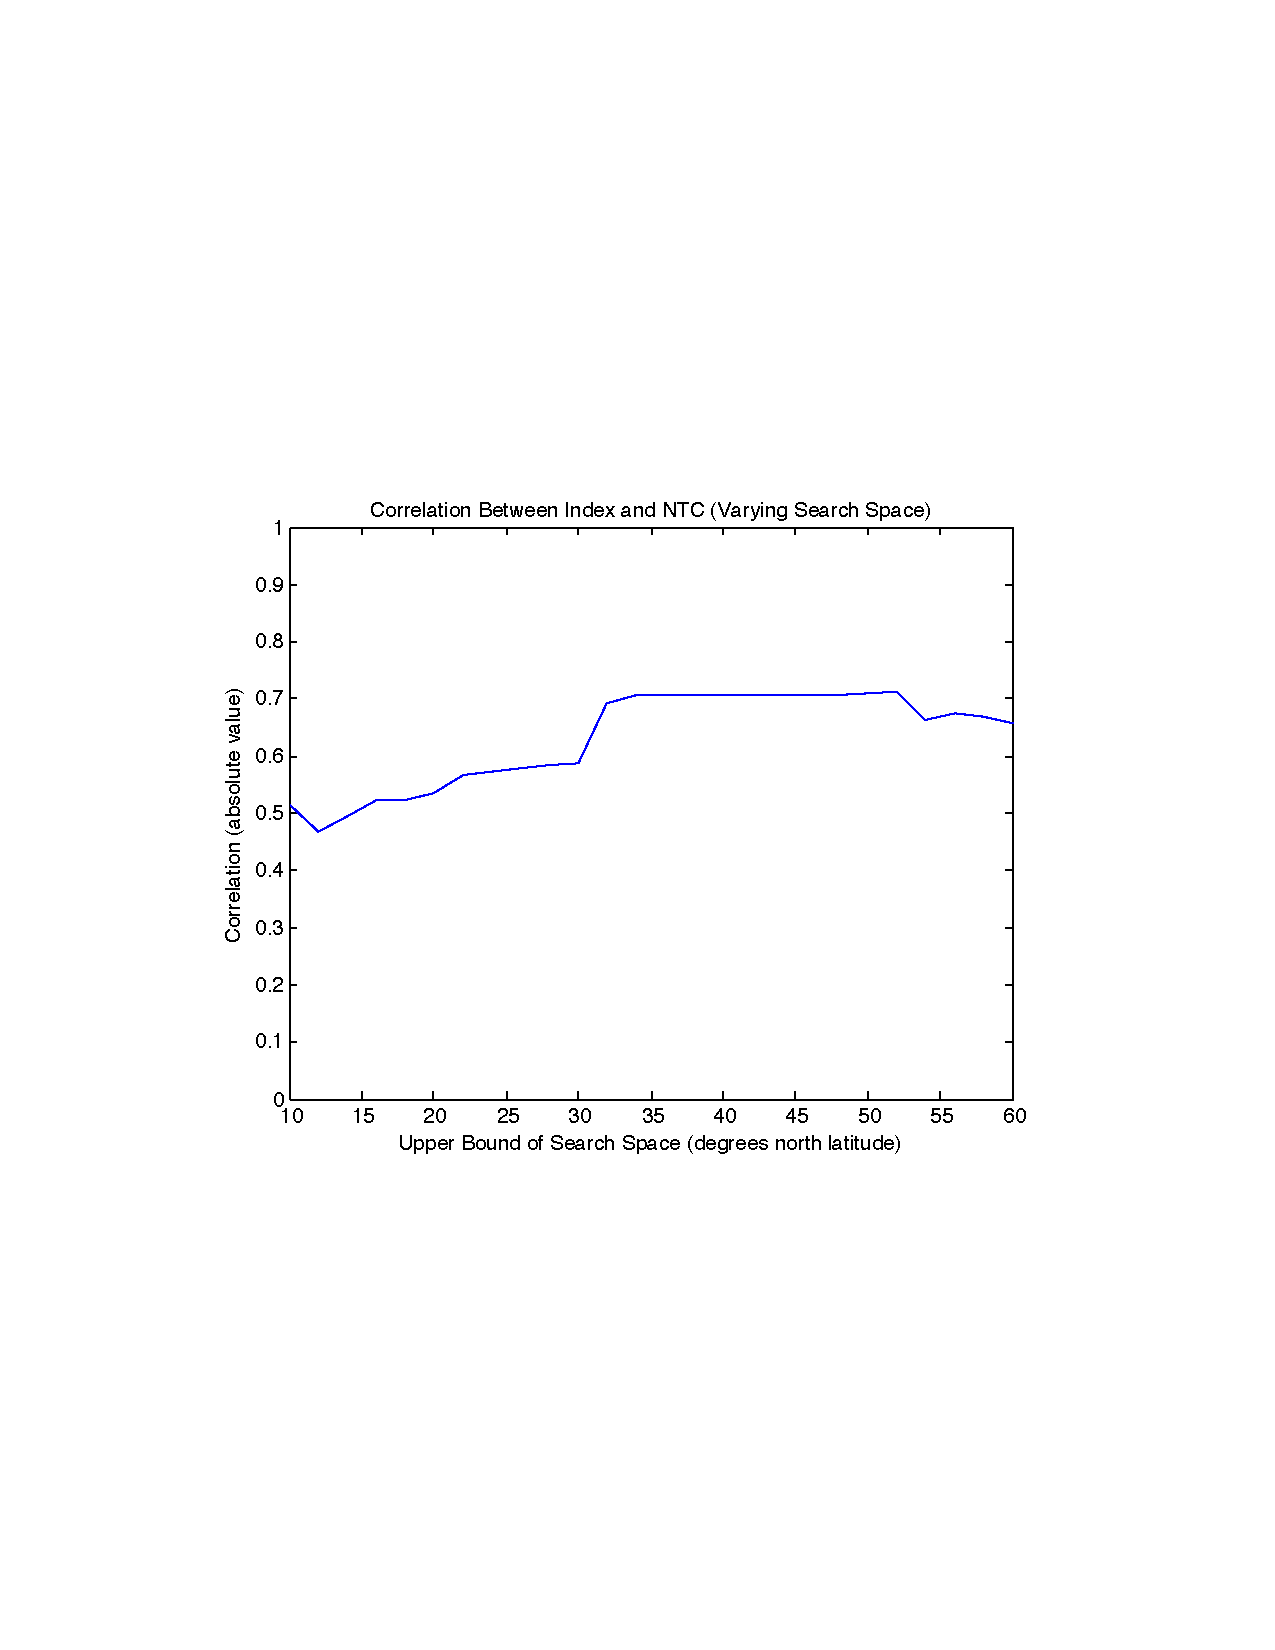
\includegraphics[width=\textwidth]{figures/sensitivityResults/northHem/NTC_Index_North.pdf}
\caption{Corr Index vs. NTC}
\label{fig:figure15}
\end{minipage}
\hspace{0cm}
\begin{minipage}[b]{0.6\linewidth}
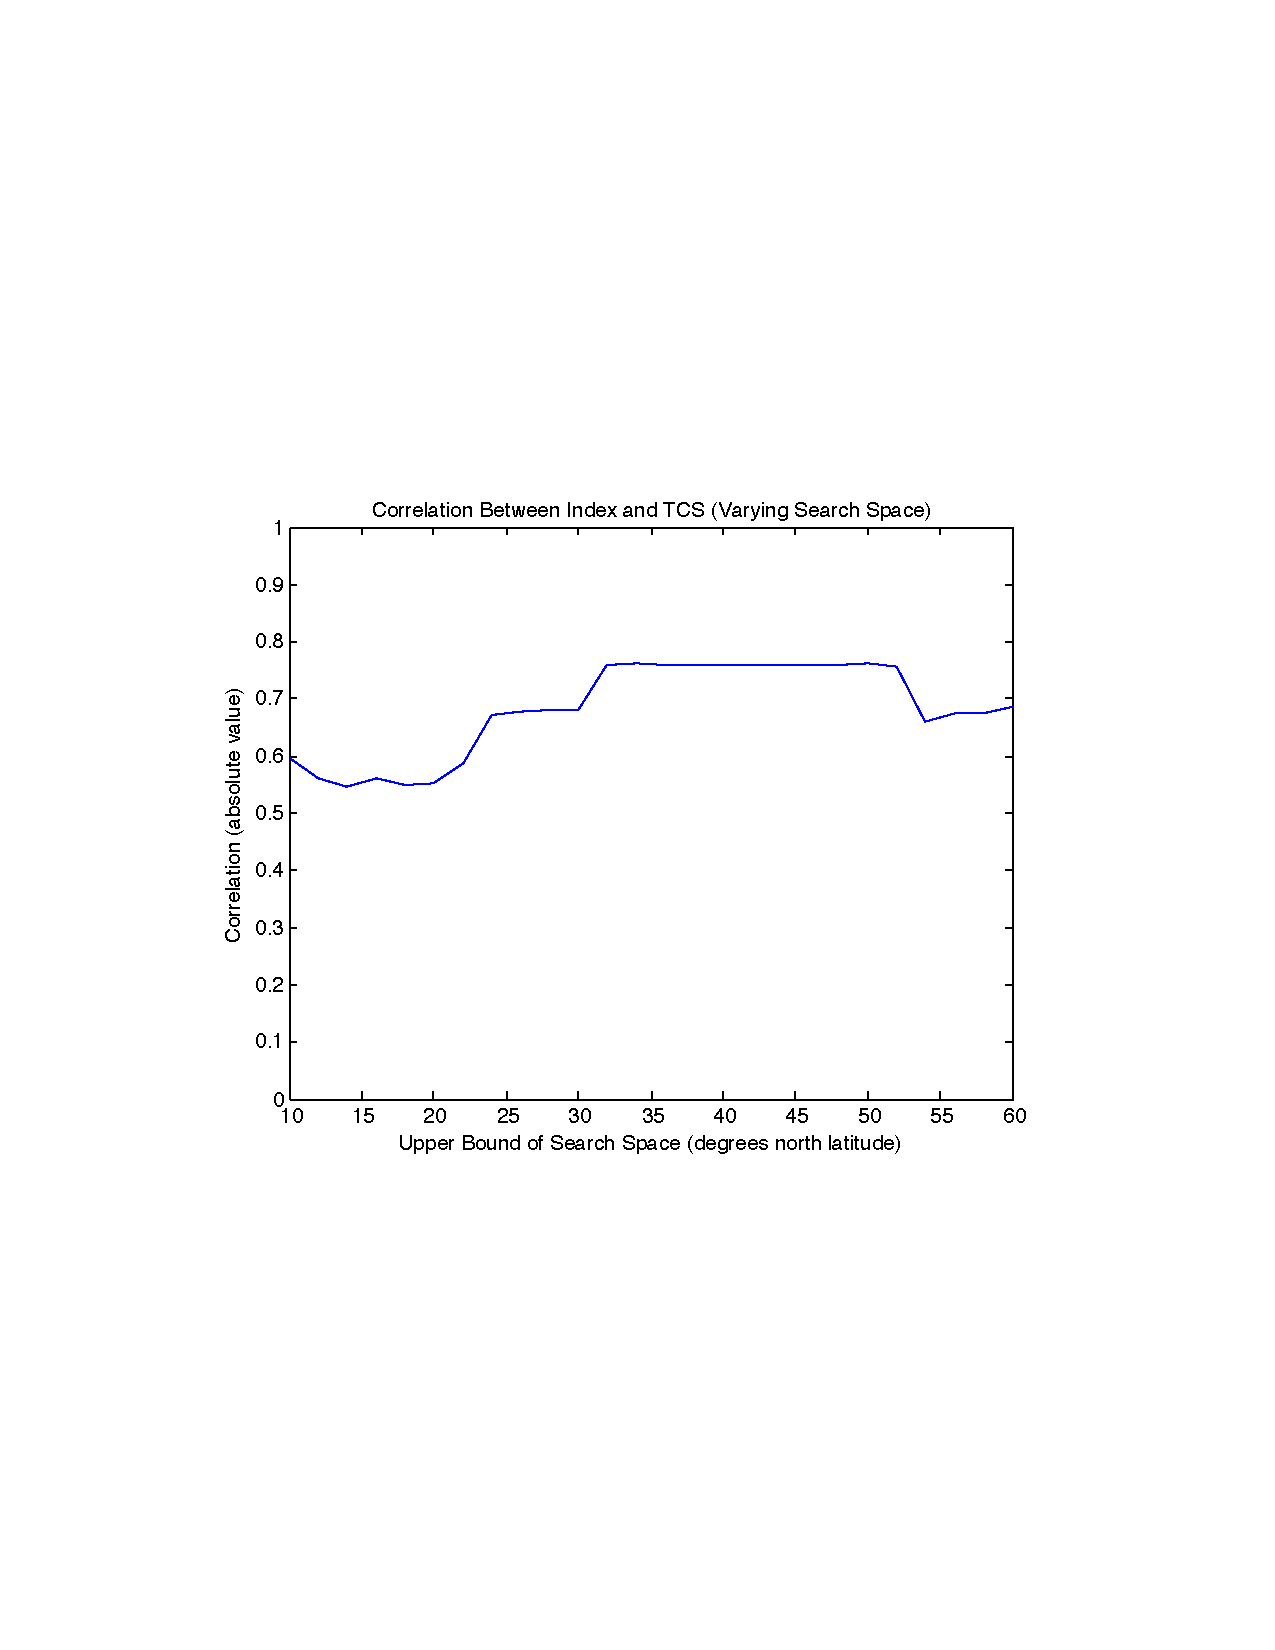
\includegraphics[width=\textwidth]{figures/sensitivityResults/northHem/TCS_Index_North.pdf}
\caption{Corr Index vs. TCs}
\label{fig:figure16}
\end{minipage}
\end{figure}
\pagebreak
\subsection{Varying Hurricane Season}

\begin{figure}[ht]
\begin{minipage}[b]{0.6\linewidth}
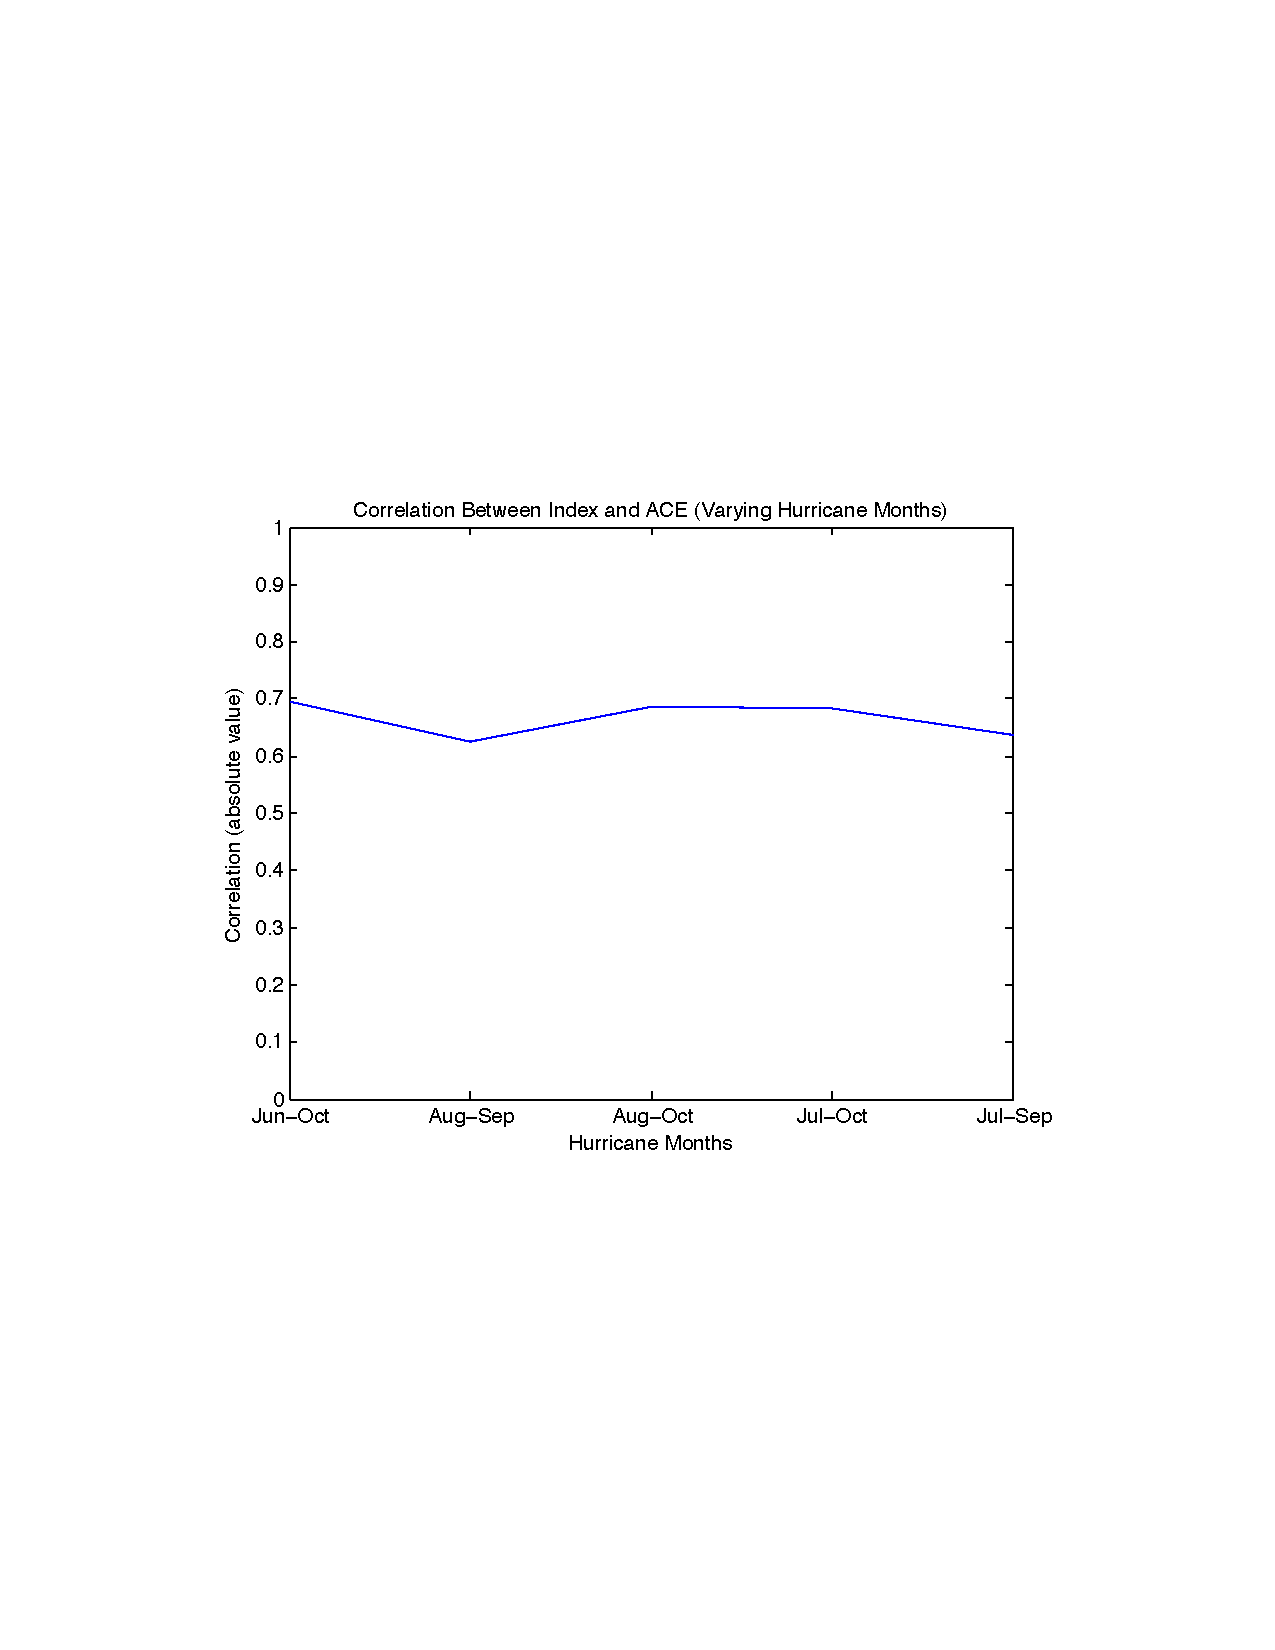
\includegraphics[width=\textwidth]{figures/sensitivityResults/hurrMonths/ACE_Index_Hurr_Months.pdf}
\caption{Corr Index vs. ACE}
\label{fig:figure17}
\end{minipage}
\hspace{0cm}
\begin{minipage}[b]{0.6\linewidth}
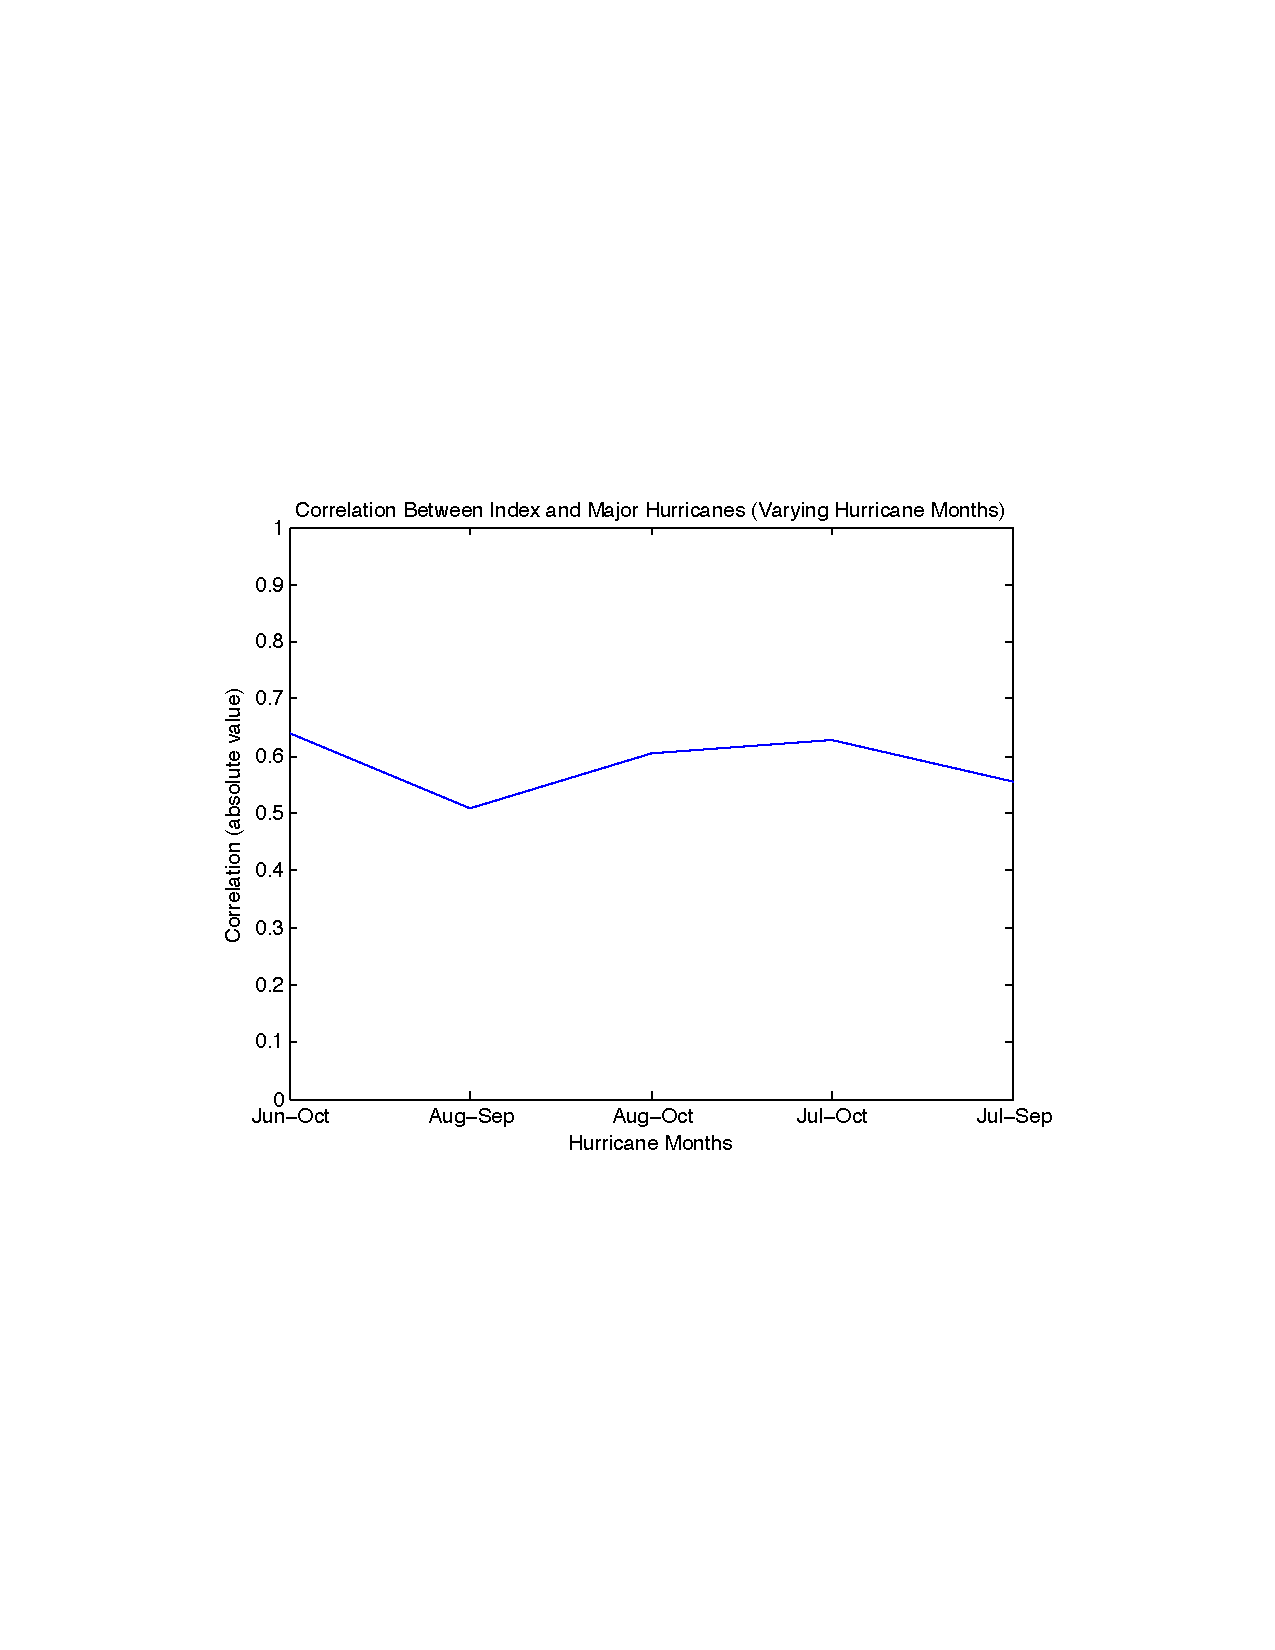
\includegraphics[width=\textwidth]{figures/sensitivityResults/hurrMonths/Major_Hurricanes_Index_Hurr_Months.pdf}
\caption{Corr Index vs. Major Hurricanes}
\label{fig:figure18}
\end{minipage}
\end{figure}
\begin{figure}[ht]
\begin{minipage}[b]{0.6\linewidth}
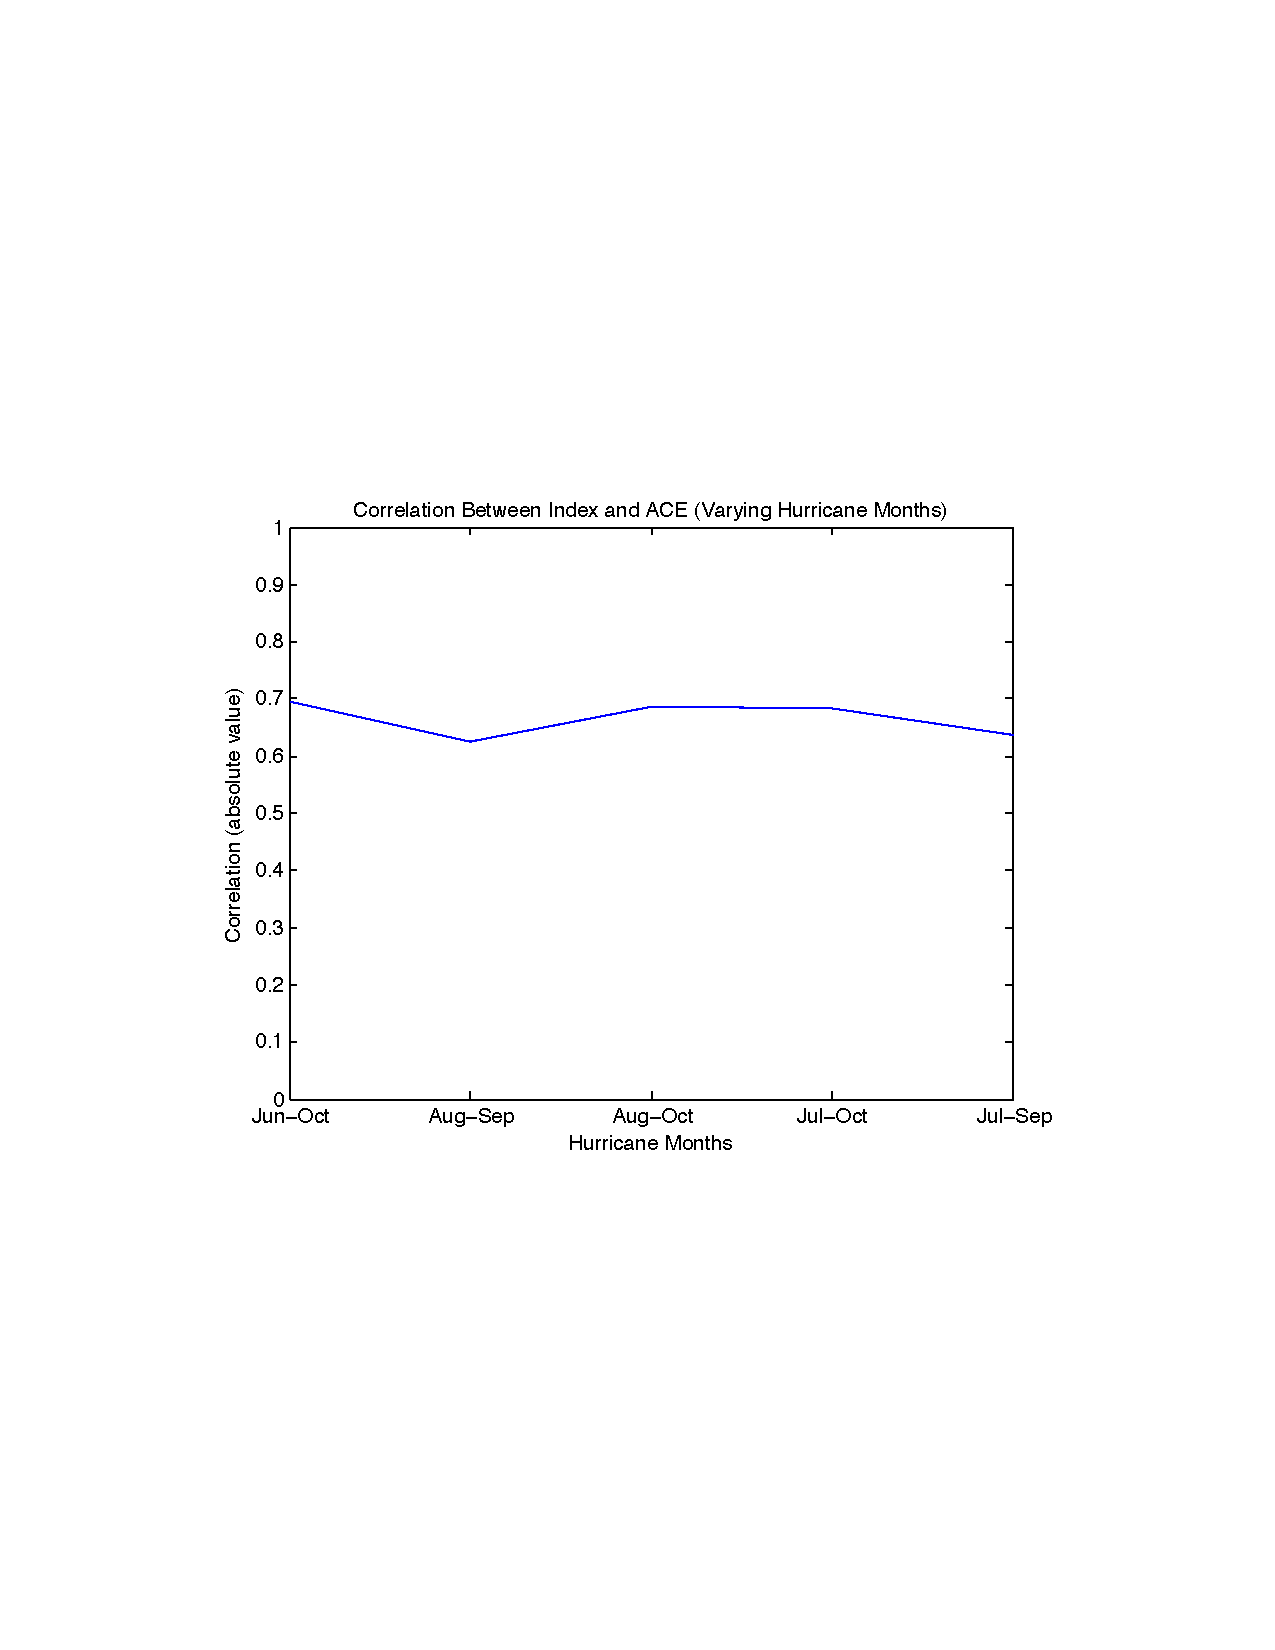
\includegraphics[width=\textwidth]{figures/sensitivityResults/hurrMonths/ACE_Index_Hurr_Months.pdf}
\caption{Corr Index vs. ACE}
\label{fig:figure19}
\end{minipage}
\hspace{0cm}
\begin{minipage}[b]{0.6\linewidth}
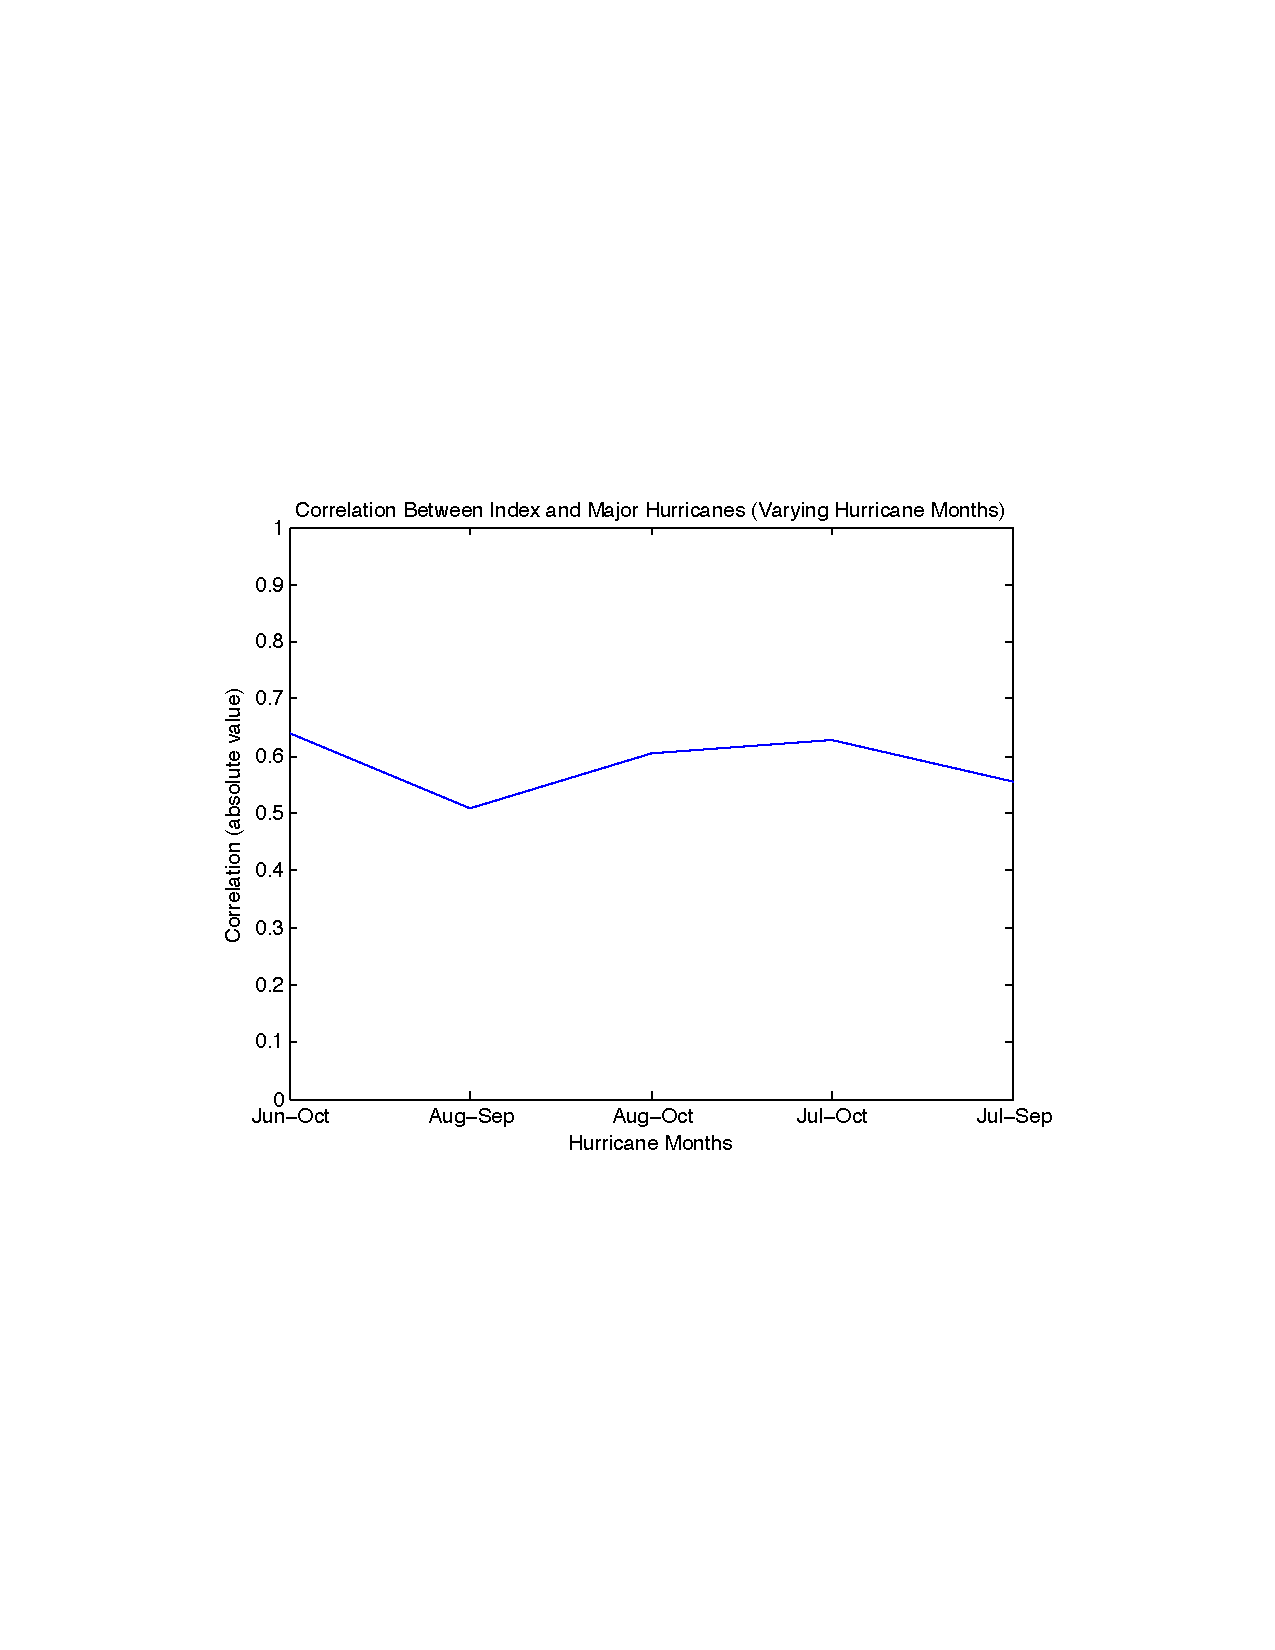
\includegraphics[width=\textwidth]{figures/sensitivityResults/hurrMonths/Major_Hurricanes_Index_Hurr_Months.pdf}
\caption{Corr Index vs. Major Hurricanes}
\label{fig:figure20}
\end{minipage}
\end{figure}

\pagebreak
\section{Difference Composite Maps}
\begin{figure}[ht]
\begin{minipage}[b]{0.55\linewidth}
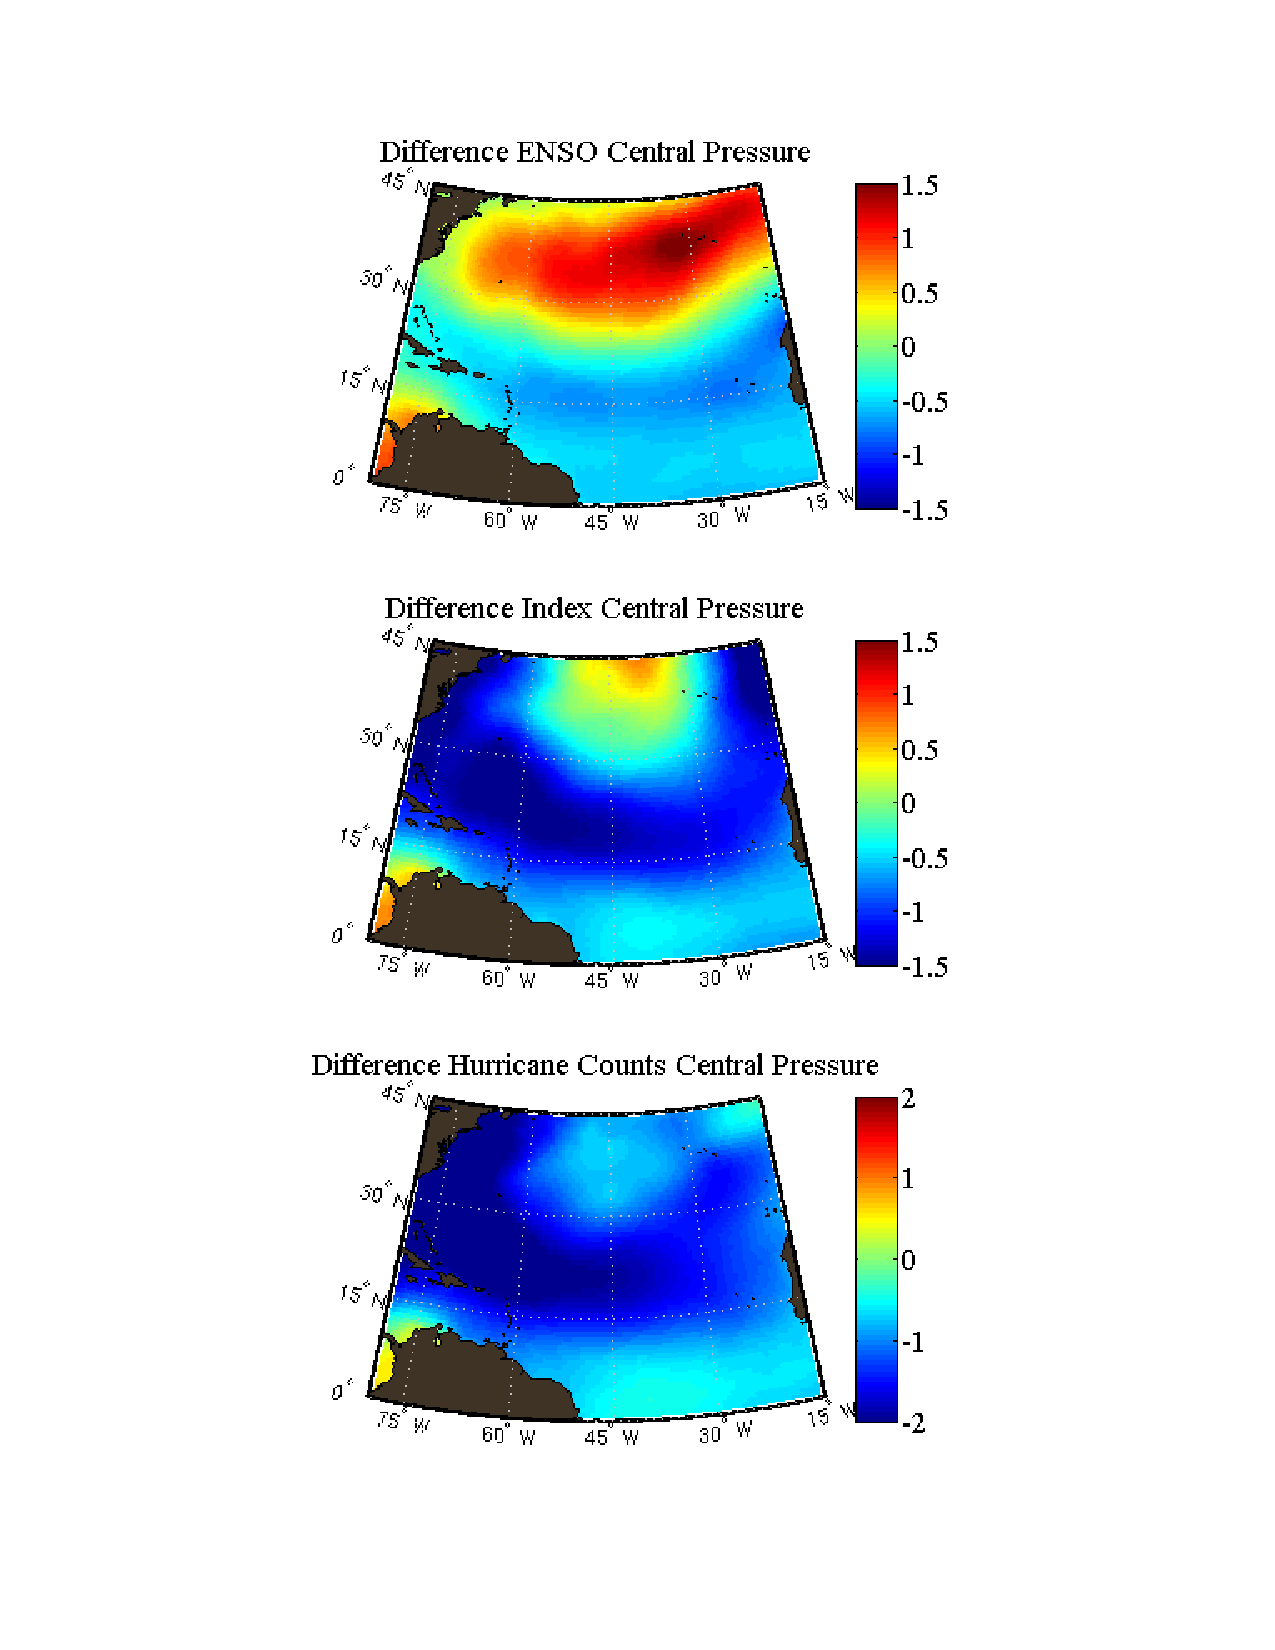
\includegraphics[width=\textwidth]{figures/sensitivityResults/compositeMaps/centralPressureAtlanticMap.pdf}
\caption{Diff Pressure Composites}
\label{fig:figure21}
\end{minipage}
\hspace{0cm}
\begin{minipage}[b]{0.55\linewidth}
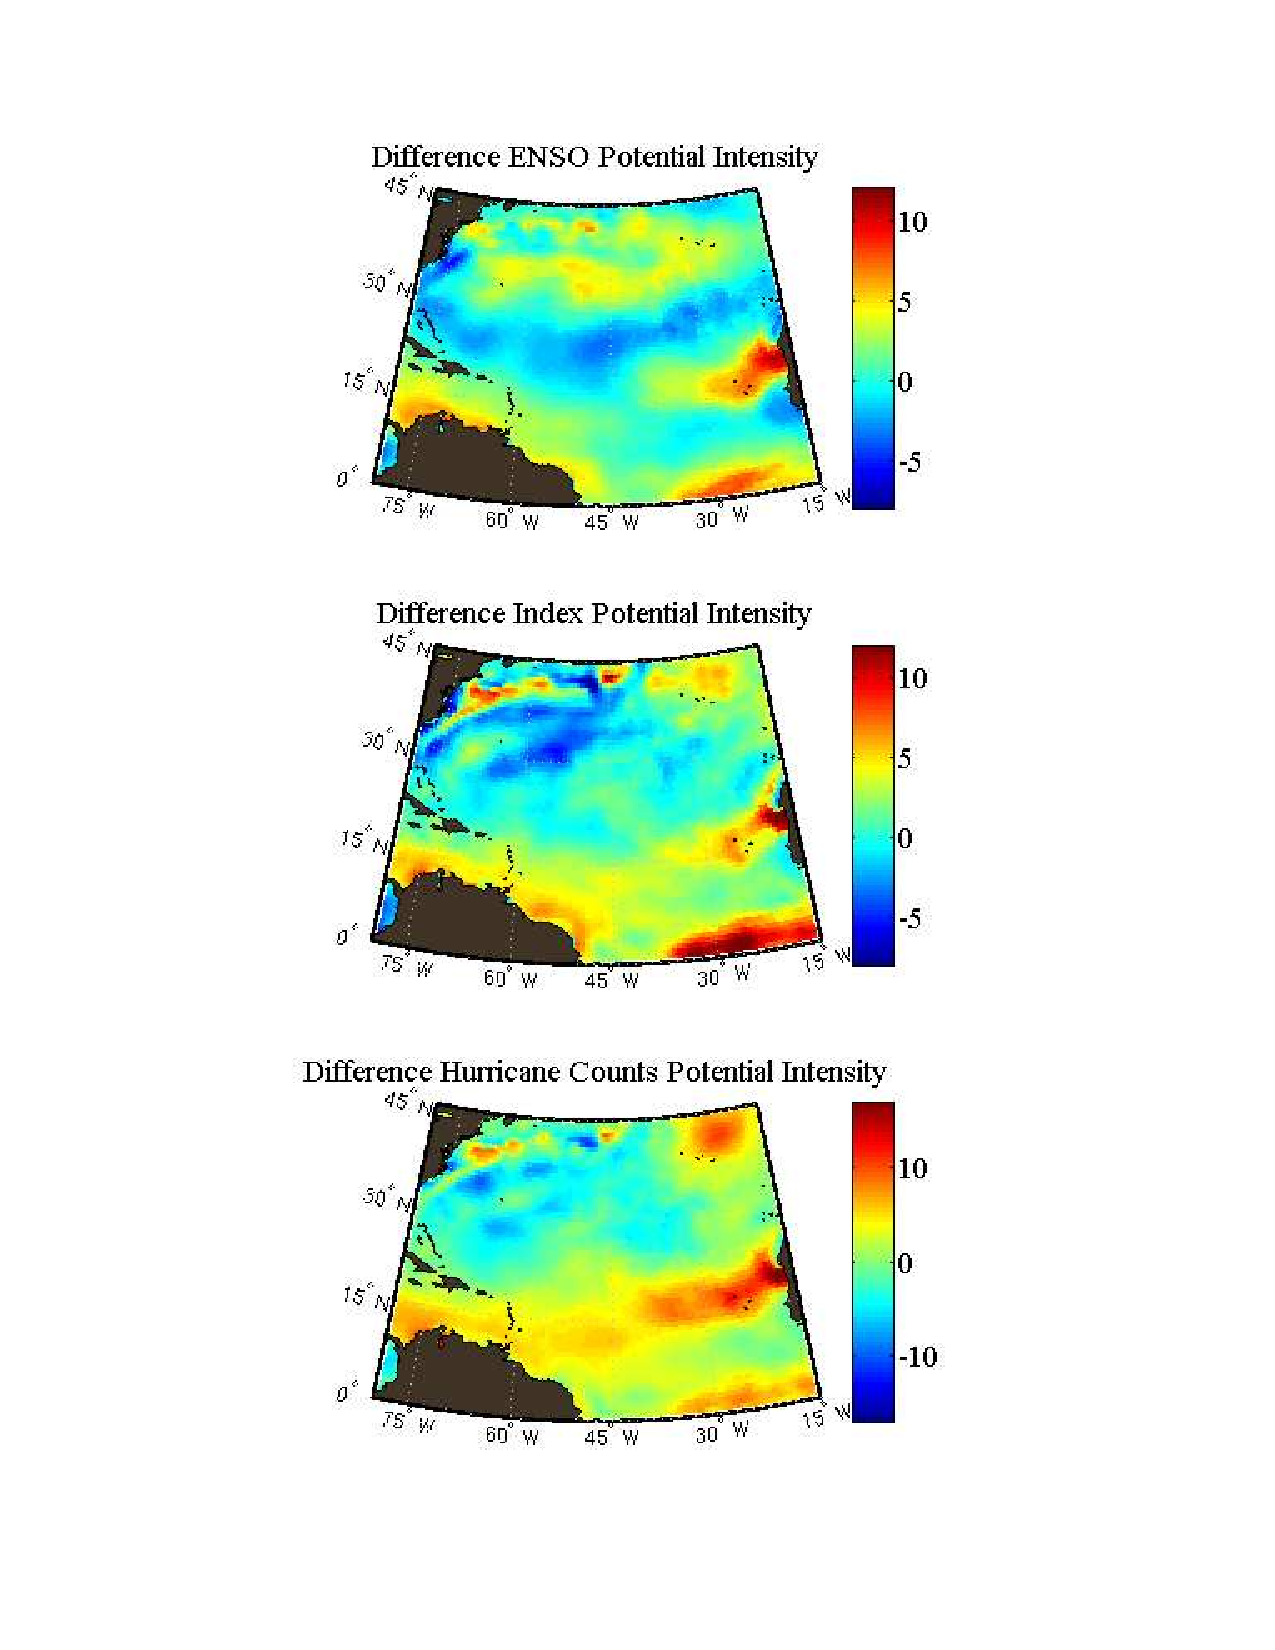
\includegraphics[width=\textwidth]{figures/sensitivityResults/compositeMaps/diffPIAtlanticComposites.pdf}
\caption{Diff PI Composites}
\label{fig:figure22}
\end{minipage}
\end{figure}

\pagebreak
\begin{figure}[ht]
\begin{minipage}[b]{0.6\linewidth}
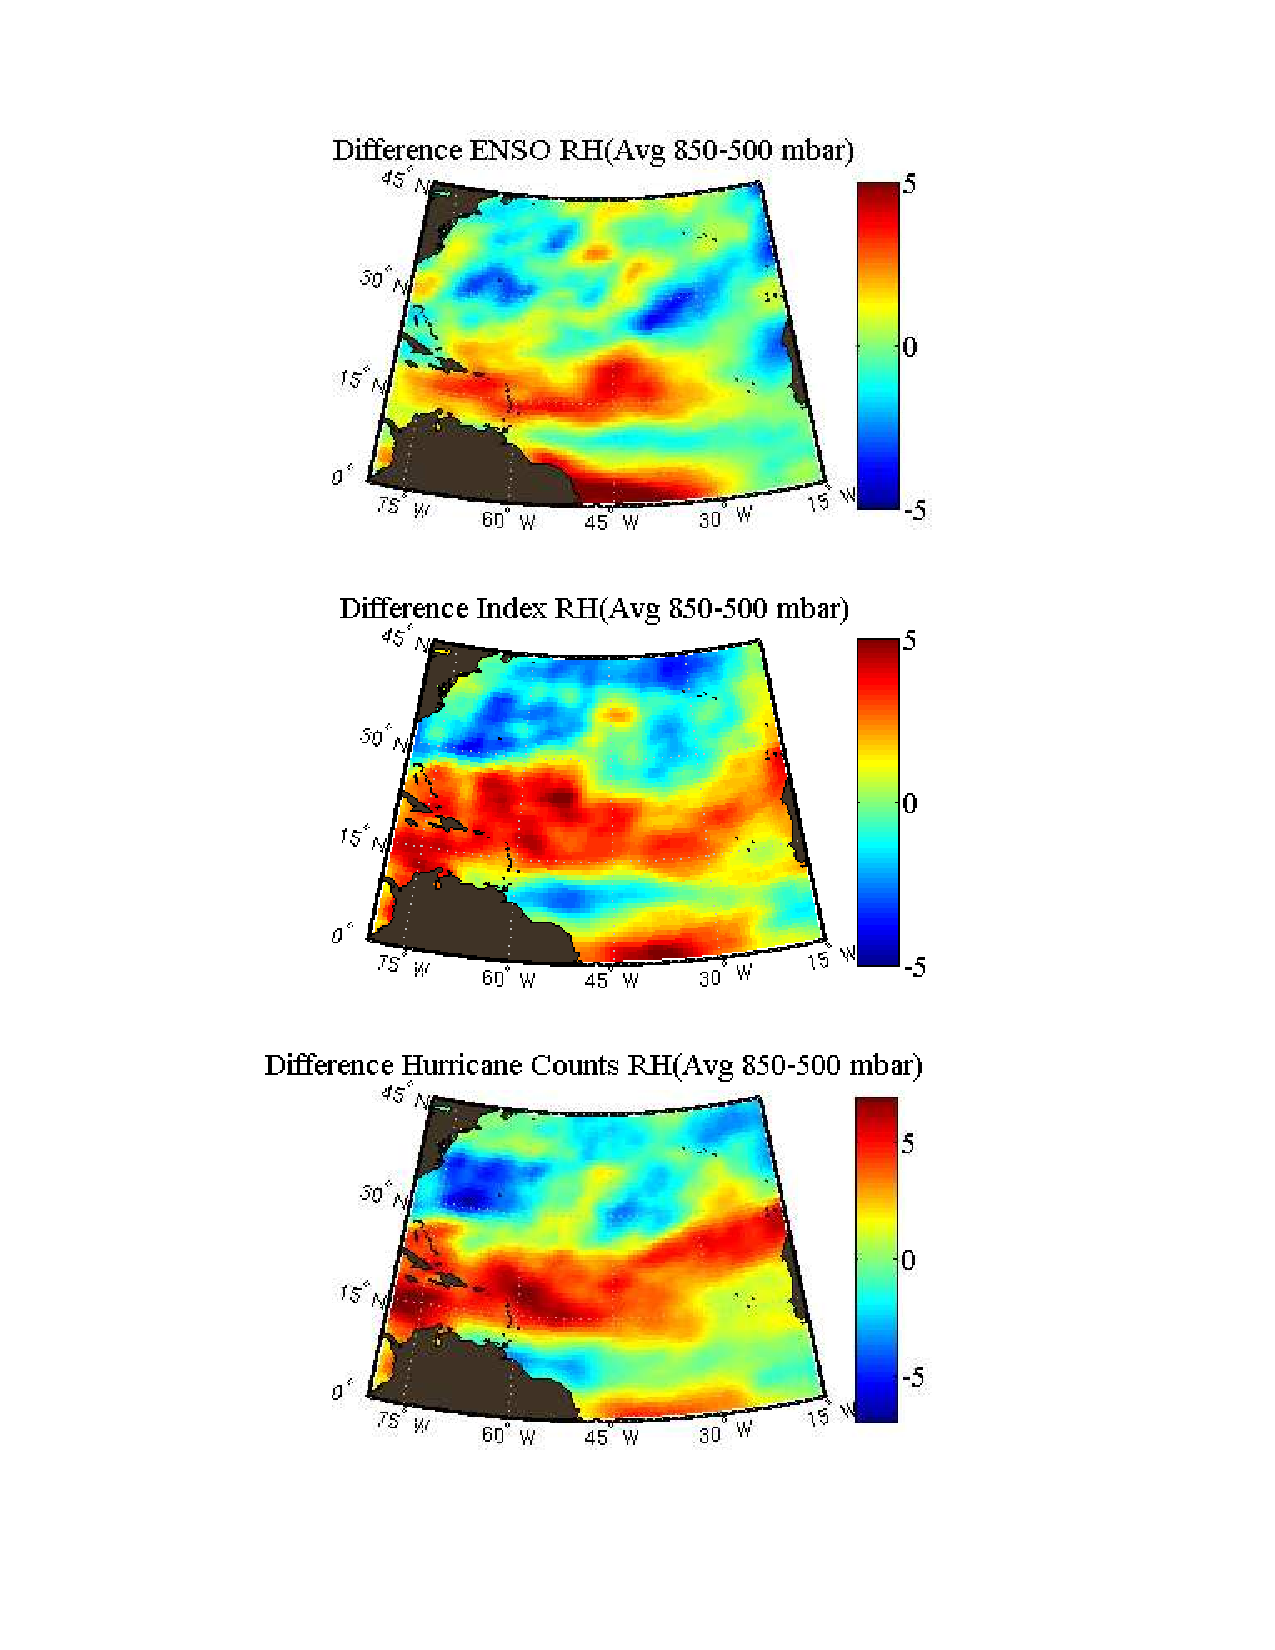
\includegraphics[width=\textwidth]{figures/sensitivityResults/compositeMaps/diffRHCompositesAtlanticMap.pdf}
\caption{Diff Relative Humidity}
\label{fig:figure23}
\end{minipage}
\hspace{0cm}
\begin{minipage}[b]{0.6\linewidth}
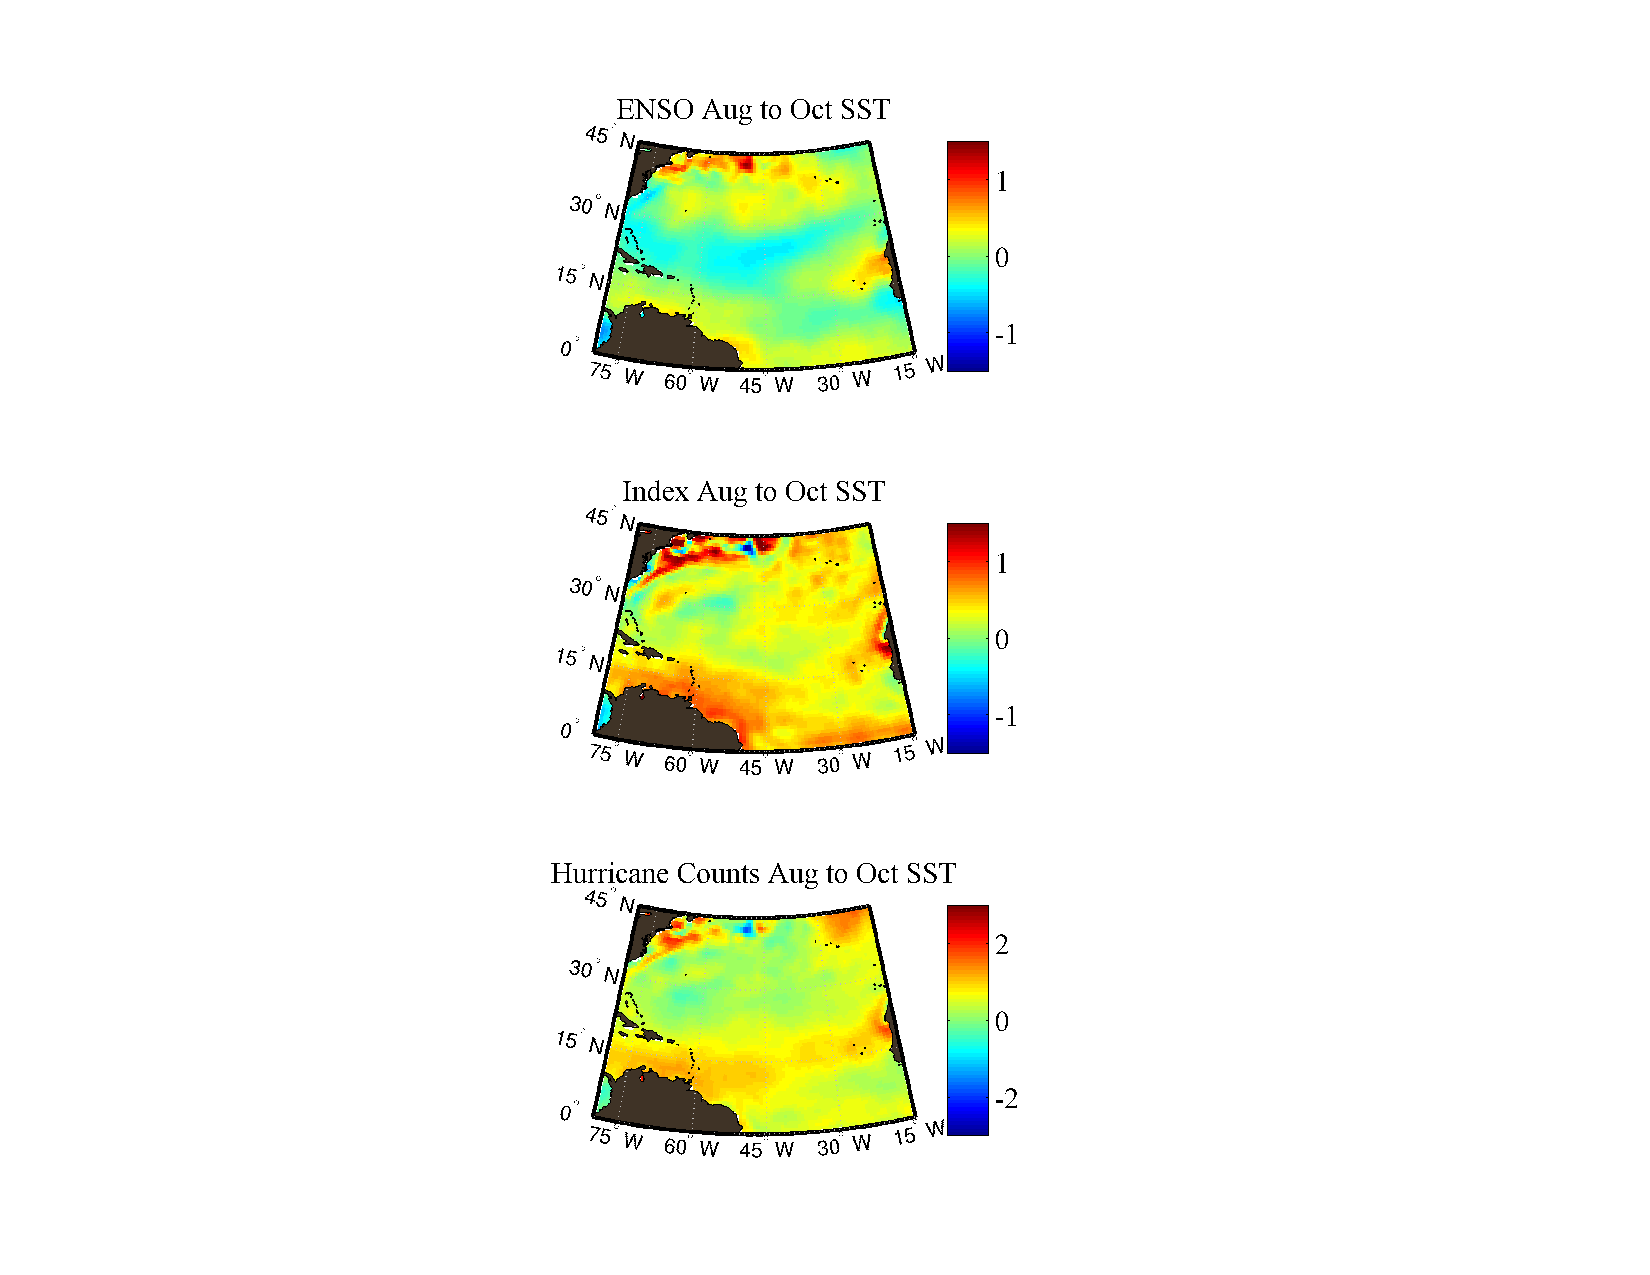
\includegraphics[width=\textwidth]{figures/sensitivityResults/compositeMaps/diffSSTCompositesAugToOct.pdf}
\caption{Diff SST Composites}
\label{fig:figure24}
\end{minipage}
\end{figure}

\pagebreak
\begin{figure}[ht]
\begin{minipage}[b]{0.6\linewidth}
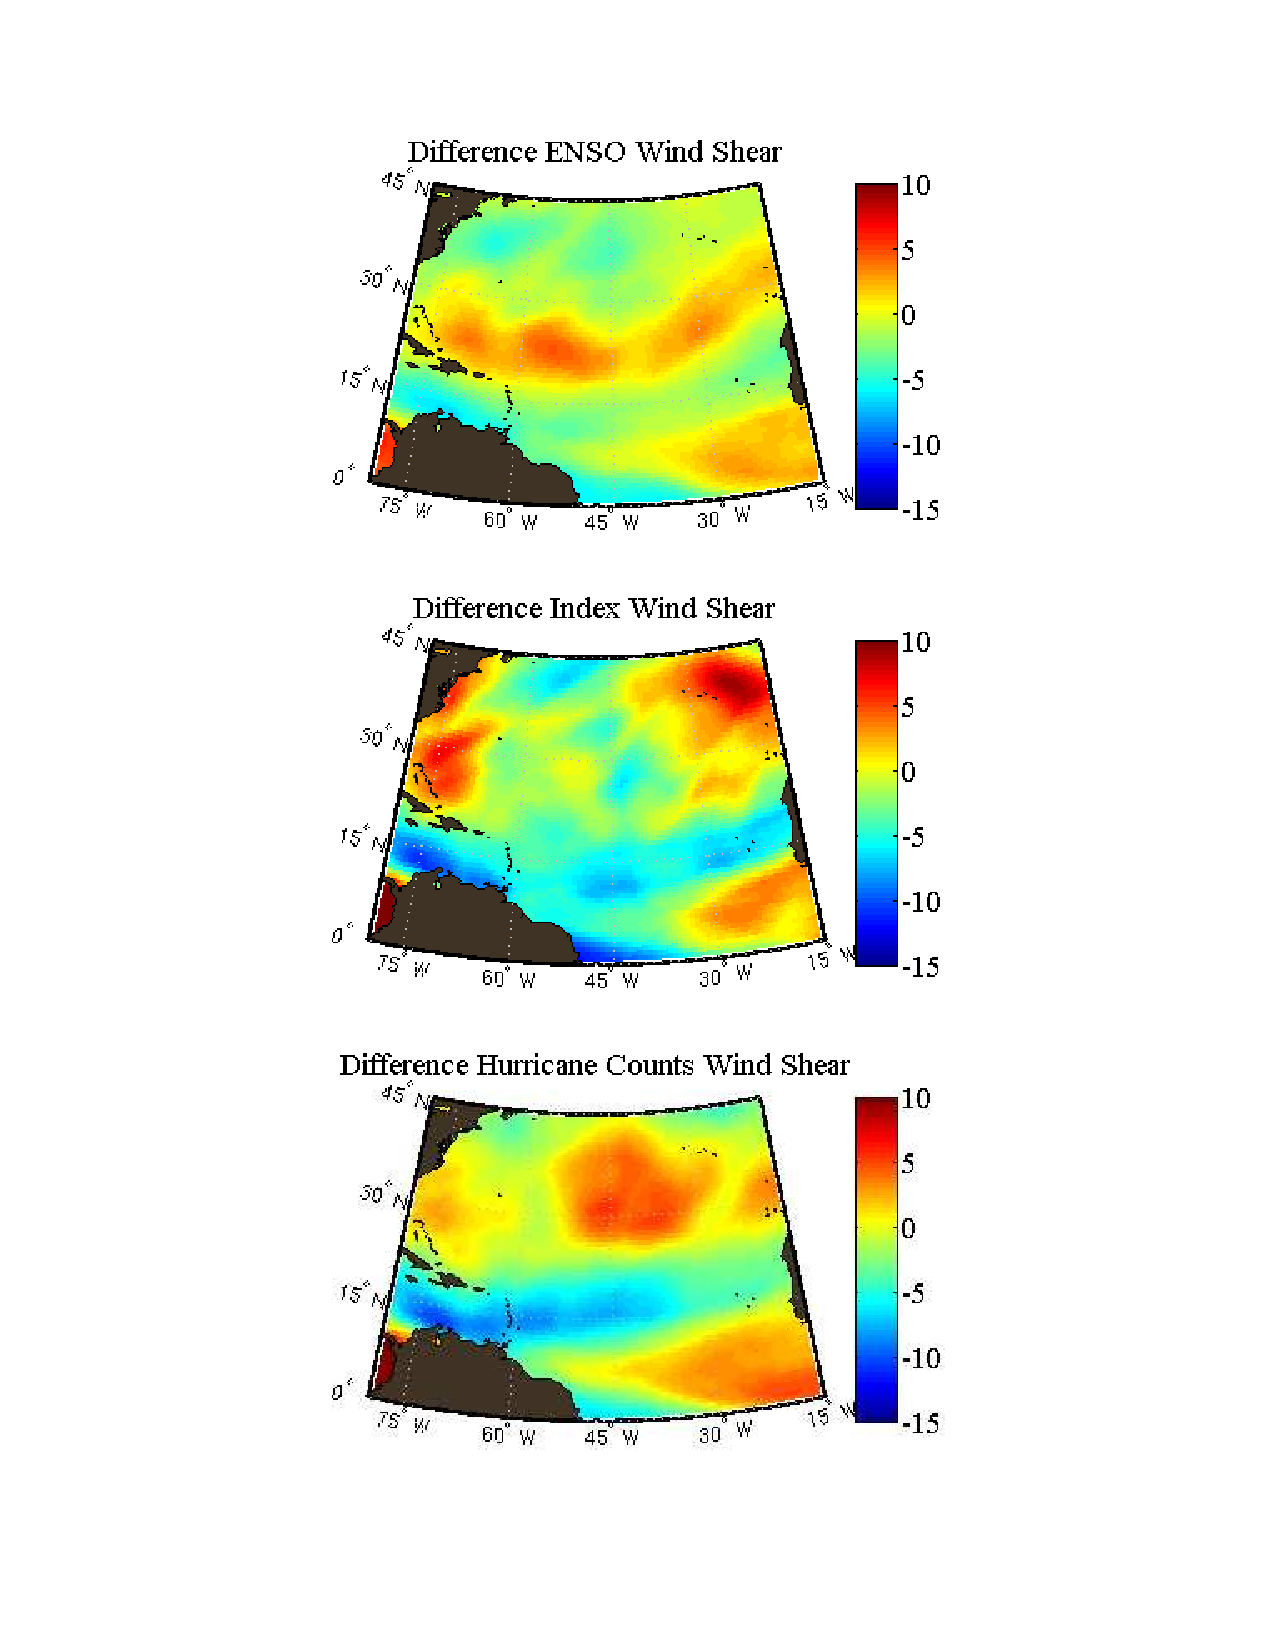
\includegraphics[width=\textwidth]{figures/sensitivityResults/compositeMaps/diffWindShearAtlanticComposites.pdf}
\caption{Diff Wind Shear}
\label{fig:figure25}
\end{minipage}
\hspace{0cm}
\begin{minipage}[b]{0.6\linewidth}
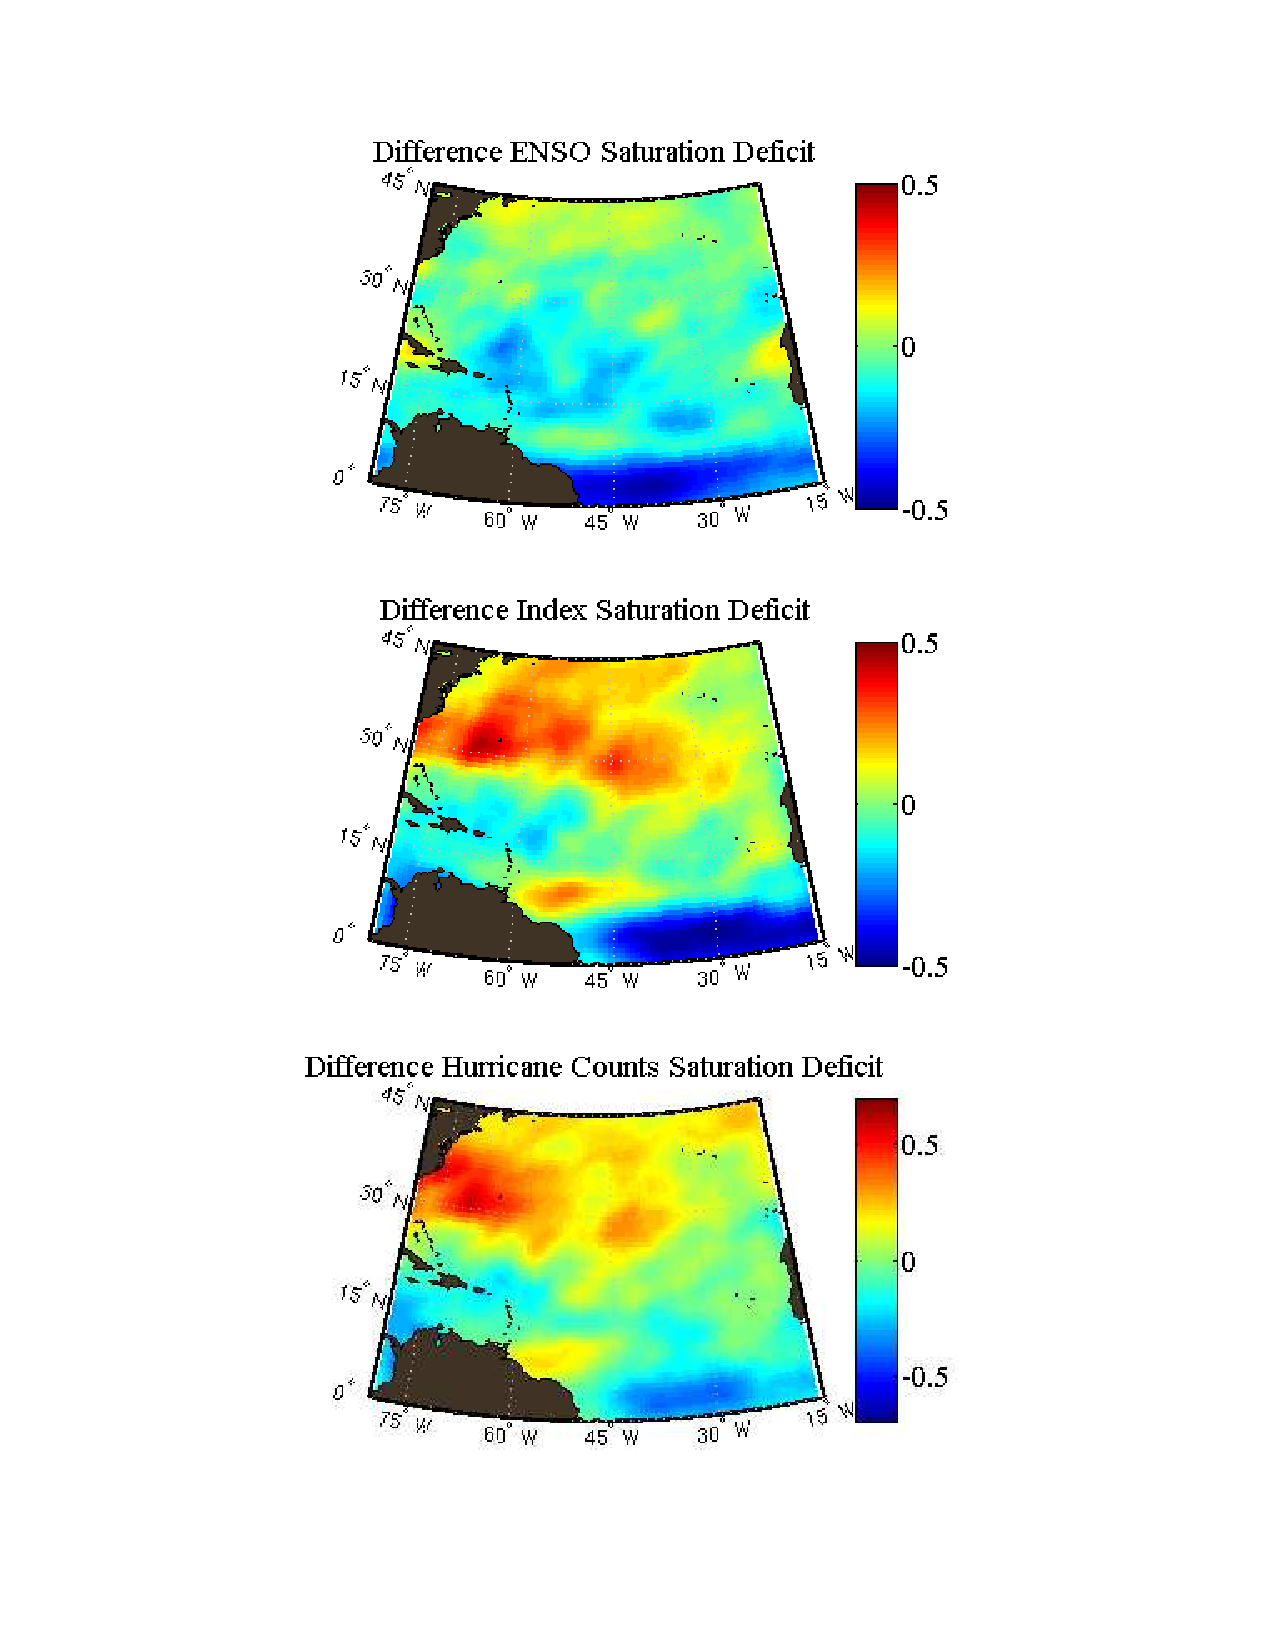
\includegraphics[width=\textwidth]{figures/sensitivityResults/compositeMaps/satDefAtlanticMap.pdf}
\caption{Diff Saturation Deficit}
\label{fig:figure26}
\end{minipage}
\end{figure}

\clearpage
\section{Average Difference Bar Graphs}
\begin{figure}[ht]
\begin{minipage}[b]{0.6\linewidth}
\includegraphics[width=\textwidth]{figures/sensitivityResults/compositeBarGraphs/RHBarGraph.pdf}
\caption{Avg Diff Relative Humidity}
\label{fig:figure27}
\end{minipage}
\hspace{0cm}
\begin{minipage}[b]{0.6\linewidth}
\includegraphics[width=\textwidth]{figures/sensitivityResults/compositeBarGraphs/avgDiffWindShearBarGraph.pdf}
\caption{Avg Diff Wind Shear (between 850-200mbar)}
\label{fig:figure28}
\end{minipage}
\end{figure}

\begin{figure}[ht]
\begin{minipage}[b]{0.6\linewidth}
\includegraphics[width=\textwidth]{figures/sensitivityResults/compositeBarGraphs/centralPressureBarGraph.pdf}
\caption{Avg Diff Central Pressure}
\label{fig:figure29}
\end{minipage}
\hspace{0cm}
\begin{minipage}[b]{0.6\linewidth}
\includegraphics[width=\textwidth]{figures/sensitivityResults/compositeBarGraphs/satDefBarGraphSmallerBox.pdf}
\caption{Avg Diff Saturation Deficit}
\label{fig:figure30}
\end{minipage}
\end{figure}
\pagebreak
\begin{figure}[ht]
\begin{minipage}[b]{0.6\linewidth}
\includegraphics[width=\textwidth]{figures/sensitivityResults/compositeBarGraphs/avgDiffPIAtlanticCompositesBarGraph.pdf}
\caption{Avg Diff Potential Intensity}
\label{fig:figure31}
\end{minipage}
\hspace{0cm}
\begin{minipage}[b]{0.6\linewidth}
\includegraphics[width=\textwidth]{figures/sensitivityResults/compositeBarGraphs/sstBarGraph.pdf}
\caption{Avg Diff SST}
\label{fig:figure32}
\end{minipage}
\end{figure}
\end{comment}

\bibliographystyle{plain1}
\bibliography{hurricanes_copy}
\end{document}
